\documentclass{book}
\usepackage[a4paper,top=2.5cm,bottom=2.5cm,left=2.5cm,right=2.5cm]{geometry}
\usepackage{makeidx}
\usepackage{natbib}
\usepackage{graphicx}
\usepackage{multicol}
\usepackage{float}
\usepackage{listings}
\usepackage{color}
\usepackage{ifthen}
\usepackage[table]{xcolor}
\usepackage{textcomp}
\usepackage{alltt}
\usepackage{ifpdf}
\ifpdf
\usepackage[pdftex,
            pagebackref=true,
            colorlinks=true,
            linkcolor=blue,
            unicode
           ]{hyperref}
\else
\usepackage[ps2pdf,
            pagebackref=true,
            colorlinks=true,
            linkcolor=blue,
            unicode
           ]{hyperref}
\usepackage{pspicture}
\fi
\usepackage[utf8]{inputenc}
\usepackage{mathptmx}
\usepackage[scaled=.90]{helvet}
\usepackage{courier}
\usepackage{sectsty}
\usepackage{amssymb}
\usepackage[titles]{tocloft}
\usepackage{doxygen}
\lstset{language=C++,inputencoding=utf8,basicstyle=\footnotesize,breaklines=true,breakatwhitespace=true,tabsize=4,numbers=left }
\makeindex
\setcounter{tocdepth}{3}
\renewcommand{\footrulewidth}{0.4pt}
\renewcommand{\familydefault}{\sfdefault}
\hfuzz=15pt
\setlength{\emergencystretch}{15pt}
\hbadness=750
\tolerance=750
\begin{document}
\hypersetup{pageanchor=false,citecolor=blue}
\begin{titlepage}
\vspace*{7cm}
\begin{center}
{\Large My Project }\\
\vspace*{1cm}
{\large Generated by Doxygen 1.8.2}\\
\vspace*{0.5cm}
{\small Tue Sep 11 2012 16:18:28}\\
\end{center}
\end{titlepage}
\clearemptydoublepage
\pagenumbering{roman}
\tableofcontents
\clearemptydoublepage
\pagenumbering{arabic}
\hypersetup{pageanchor=true,citecolor=blue}
\chapter{example}
\label{example}
\hypertarget{example}{}
 Our main function starts like this\-: 
\begin{DoxyCodeInclude}

\end{DoxyCodeInclude}
 First we create a object {\ttfamily t} of the \hyperlink{class_test}{Test} class. 
\begin{DoxyCodeInclude}

\end{DoxyCodeInclude}
 Then we call the example member function 
\begin{DoxyCodeInclude}

\end{DoxyCodeInclude}
 After that our little test routine ends. 
\begin{DoxyCodeInclude}

\end{DoxyCodeInclude}
 
\chapter{Bug List}
\label{bug}
\hypertarget{bug}{}

\begin{DoxyRefList}
\item[\label{bug__bug000001}%
\hypertarget{bug__bug000001}{}%
Class \hyperlink{class_some_nice_class}{Some\-Nice\-Class} ]Not all memory is freed when deleting an object of this class. 
\end{DoxyRefList}
\chapter{Module Index}
\section{Modules}
Here is a list of all modules\-:\begin{DoxyCompactList}
\item \contentsline{section}{The First Group}{\pageref{group__group1}}{}
\item \contentsline{section}{The Second Group}{\pageref{group__group2}}{}
\item \contentsline{section}{The Third Group}{\pageref{group__group3}}{}
\begin{DoxyCompactList}
\item \contentsline{section}{The Fourth Group}{\pageref{group__group4}}{}
\end{DoxyCompactList}
\item \contentsline{section}{The Fifth Group}{\pageref{group__group5}}{}
\end{DoxyCompactList}

\chapter{Namespace Index}
\section{Namespace List}
Here is a list of all documented namespaces with brief descriptions\-:\begin{DoxyCompactList}
\item\contentsline{section}{\hyperlink{namespacedocstring}{docstring} }{\pageref{namespacedocstring}}{}
\item\contentsline{section}{\hyperlink{namespace_n1}{N1} }{\pageref{namespace_n1}}{}
\item\contentsline{section}{\hyperlink{namespacens}{ns} }{\pageref{namespacens}}{}
\item\contentsline{section}{\hyperlink{namespacepyexample}{pyexample} \\*Documentation for this module }{\pageref{namespacepyexample}}{}
\end{DoxyCompactList}

\chapter{Hierarchical Index}
\section{Class Hierarchy}
This inheritance list is sorted roughly, but not completely, alphabetically\-:\begin{DoxyCompactList}
\item \contentsline{section}{A}{\pageref{class_a}}{}
\begin{DoxyCompactList}
\item \contentsline{section}{C}{\pageref{class_c}}{}
\item \contentsline{section}{D}{\pageref{class_d}}{}
\begin{DoxyCompactList}
\item \contentsline{section}{E}{\pageref{class_e}}{}
\end{DoxyCompactList}
\end{DoxyCompactList}
\item \contentsline{section}{B}{\pageref{class_b}}{}
\begin{DoxyCompactList}
\item \contentsline{section}{D}{\pageref{class_d}}{}
\end{DoxyCompactList}
\item \contentsline{section}{C1}{\pageref{class_c1}}{}
\item \contentsline{section}{C2}{\pageref{class_c2}}{}
\item \contentsline{section}{C3}{\pageref{class_c3}}{}
\item \contentsline{section}{C4}{\pageref{class_c4}}{}
\item \contentsline{section}{C5}{\pageref{class_c5}}{}
\item \contentsline{section}{Coord\-Struct}{\pageref{struct_coord_struct}}{}
\item \contentsline{section}{ns\-:\-:itcl\-\_\-class}{\pageref{classns_1_1itcl__class}}{}
\item \contentsline{section}{mux\-\_\-using\-\_\-with}{\pageref{classmux__using__with}}{}
\item \contentsline{section}{Object}{\pageref{struct_object}}{}
\begin{DoxyCompactList}
\item \contentsline{section}{Vehicle}{\pageref{struct_vehicle}}{}
\begin{DoxyCompactList}
\item \contentsline{section}{Car}{\pageref{struct_car}}{}
\item \contentsline{section}{Truck}{\pageref{struct_truck}}{}
\end{DoxyCompactList}
\end{DoxyCompactList}
\item \contentsline{section}{ns\-:\-:oo\-\_\-class}{\pageref{classns_1_1oo__class}}{}
\item \contentsline{section}{docstring.\-Py\-Class}{\pageref{classdocstring_1_1_py_class}}{}
\item \contentsline{section}{pyexample.\-Py\-Class}{\pageref{classpyexample_1_1_py_class}}{}
\item \contentsline{section}{Some\-Nice\-Class}{\pageref{class_some_nice_class}}{}
\item \contentsline{section}{String}{\pageref{class_string}}{}
\item \contentsline{section}{Test$<$ T, i $>$}{\pageref{class_test}}{}
\begin{DoxyCompactList}
\item \contentsline{section}{Tag}{\pageref{class_tag}}{}
\end{DoxyCompactList}
\item \contentsline{section}{Test$<$ void $\ast$, 200 $>$}{\pageref{class_test_3_01void_01_5_00_01200_01_4}}{}
\begin{DoxyCompactList}
\item \contentsline{section}{Test$<$ T $\ast$ $>$}{\pageref{class_test_3_01_t_01_5_01_4}}{}
\end{DoxyCompactList}
\end{DoxyCompactList}

\chapter{Class Index}
\section{Class List}
Here are the classes, structs, unions and interfaces with brief descriptions\-:\begin{DoxyCompactList}
\item\contentsline{section}{\hyperlink{class_a}{A} }{\pageref{class_a}}{}
\item\contentsline{section}{\hyperlink{class_b}{B} }{\pageref{class_b}}{}
\item\contentsline{section}{\hyperlink{class_c}{C} }{\pageref{class_c}}{}
\item\contentsline{section}{\hyperlink{class_c1}{C1} \\*Class \hyperlink{class_c1}{C1} in group 1 }{\pageref{class_c1}}{}
\item\contentsline{section}{\hyperlink{class_c2}{C2} \\*Class \hyperlink{class_c2}{C2} in group 1 }{\pageref{class_c2}}{}
\item\contentsline{section}{\hyperlink{class_c3}{C3} \\*Class \hyperlink{class_c3}{C3} in group 2 }{\pageref{class_c3}}{}
\item\contentsline{section}{\hyperlink{class_c4}{C4} \\*Class \hyperlink{class_c4}{C4} in group 2 }{\pageref{class_c4}}{}
\item\contentsline{section}{\hyperlink{class_c5}{C5} \\*Class \hyperlink{class_c5}{C5} in \hyperlink{group__group3}{the third group} }{\pageref{class_c5}}{}
\item\contentsline{section}{\hyperlink{struct_car}{Car} }{\pageref{struct_car}}{}
\item\contentsline{section}{\hyperlink{struct_coord_struct}{Coord\-Struct} }{\pageref{struct_coord_struct}}{}
\item\contentsline{section}{\hyperlink{class_d}{D} }{\pageref{class_d}}{}
\item\contentsline{section}{\hyperlink{class_e}{E} }{\pageref{class_e}}{}
\item\contentsline{section}{\hyperlink{classns_1_1itcl__class}{ns\-::itcl\-\_\-class} }{\pageref{classns_1_1itcl__class}}{}
\item\contentsline{section}{entity \hyperlink{classmux__using__with}{mux\-\_\-using\-\_\-with} \\*Mux entity brief description }{\pageref{classmux__using__with}}{}
\item\contentsline{section}{\hyperlink{struct_object}{Object} }{\pageref{struct_object}}{}
\item\contentsline{section}{\hyperlink{classns_1_1oo__class}{ns\-::oo\-\_\-class} }{\pageref{classns_1_1oo__class}}{}
\item\contentsline{section}{\hyperlink{classdocstring_1_1_py_class}{docstring.\-Py\-Class} }{\pageref{classdocstring_1_1_py_class}}{}
\item\contentsline{section}{\hyperlink{classpyexample_1_1_py_class}{pyexample.\-Py\-Class} \\*Documentation for a class }{\pageref{classpyexample_1_1_py_class}}{}
\item\contentsline{section}{\hyperlink{class_some_nice_class}{Some\-Nice\-Class} \\*Pretty nice class }{\pageref{class_some_nice_class}}{}
\item\contentsline{section}{\hyperlink{class_string}{String} }{\pageref{class_string}}{}
\item\contentsline{section}{\hyperlink{class_tag}{Tag} }{\pageref{class_tag}}{}
\item\contentsline{section}{\hyperlink{class_test}{Test$<$ T, i $>$} \\*This is a test class }{\pageref{class_test}}{}
\item\contentsline{section}{\hyperlink{class_test_3_01_t_01_5_01_4}{Test$<$ T $\ast$ $>$} }{\pageref{class_test_3_01_t_01_5_01_4}}{}
\item\contentsline{section}{\hyperlink{class_test_3_01void_01_5_00_01200_01_4}{Test$<$ void $\ast$, 200 $>$} }{\pageref{class_test_3_01void_01_5_00_01200_01_4}}{}
\item\contentsline{section}{\hyperlink{struct_truck}{Truck} }{\pageref{struct_truck}}{}
\item\contentsline{section}{\hyperlink{struct_vehicle}{Vehicle} }{\pageref{struct_vehicle}}{}
\end{DoxyCompactList}

\chapter{File Index}
\section{File List}
Here is a list of all documented files with brief descriptions\-:\begin{DoxyCompactList}
\item\contentsline{section}{\hyperlink{file_8h}{file.\-h} \\*A brief file description }{\pageref{file_8h}}{}
\end{DoxyCompactList}

\chapter{Module Documentation}
\hypertarget{group__group1}{\section{The First Group}
\label{group__group1}\index{The First Group@{The First Group}}
}
\subsection*{Namespaces}
\begin{DoxyCompactItemize}
\item 
namespace \hyperlink{namespace_n1}{N1}
\end{DoxyCompactItemize}
\subsection*{Classes}
\begin{DoxyCompactItemize}
\item 
class \hyperlink{class_c1}{C1}
\begin{DoxyCompactList}\small\item\em class \hyperlink{class_c1}{C1} in group 1 \end{DoxyCompactList}\item 
class \hyperlink{class_c2}{C2}
\begin{DoxyCompactList}\small\item\em class \hyperlink{class_c2}{C2} in group 1 \end{DoxyCompactList}\end{DoxyCompactItemize}
\subsection*{Functions}
\begin{DoxyCompactItemize}
\item 
void \hyperlink{group__group1_ga24f647174760cac13d2624b5ad74b00c}{func} ()
\item 
void \hyperlink{group__group1_ga053929c0809a5f56f7548fd7d9968f31}{func2} ()
\item 
void \hyperlink{group__group1_gadbf675591ff057ec48ce35b0d5cdf755}{func3} ()
\end{DoxyCompactItemize}


\subsection{Detailed Description}
This is the first group

More documentation for the first group. 

\subsection{Function Documentation}
\hypertarget{group__group1_ga24f647174760cac13d2624b5ad74b00c}{\index{The First Group@{The First Group}!func@{func}}
\index{func@{func}!The First Group@{The First Group}}
\subsubsection[{func}]{\setlength{\rightskip}{0pt plus 5cm}void func (
\begin{DoxyParamCaption}
{}
\end{DoxyParamCaption}
)}}\label{group__group1_ga24f647174760cac13d2624b5ad74b00c}
function in group 1 \hypertarget{group__group1_ga053929c0809a5f56f7548fd7d9968f31}{\index{The First Group@{The First Group}!func2@{func2}}
\index{func2@{func2}!The First Group@{The First Group}}
\subsubsection[{func2}]{\setlength{\rightskip}{0pt plus 5cm}void func2 (
\begin{DoxyParamCaption}
{}
\end{DoxyParamCaption}
)}}\label{group__group1_ga053929c0809a5f56f7548fd7d9968f31}
another function in group 1 \hypertarget{group__group1_gadbf675591ff057ec48ce35b0d5cdf755}{\index{The First Group@{The First Group}!func3@{func3}}
\index{func3@{func3}!The First Group@{The First Group}}
\subsubsection[{func3}]{\setlength{\rightskip}{0pt plus 5cm}void func3 (
\begin{DoxyParamCaption}
{}
\end{DoxyParamCaption}
)}}\label{group__group1_gadbf675591ff057ec48ce35b0d5cdf755}
yet another function in group 1 
\hypertarget{group__group2}{\section{The Second Group}
\label{group__group2}\index{The Second Group@{The Second Group}}
}
\subsection*{Namespaces}
\begin{DoxyCompactItemize}
\item 
namespace \hyperlink{namespace_n1}{N1}
\end{DoxyCompactItemize}
\subsection*{Classes}
\begin{DoxyCompactItemize}
\item 
class \hyperlink{class_c3}{C3}
\begin{DoxyCompactList}\small\item\em class \hyperlink{class_c3}{C3} in group 2 \end{DoxyCompactList}\item 
class \hyperlink{class_c4}{C4}
\begin{DoxyCompactList}\small\item\em class \hyperlink{class_c4}{C4} in group 2 \end{DoxyCompactList}\end{DoxyCompactItemize}


\subsection{Detailed Description}
This is the second group 
\hypertarget{group__group3}{\section{The Third Group}
\label{group__group3}\index{The Third Group@{The Third Group}}
}
\subsection*{Modules}
\begin{DoxyCompactItemize}
\item 
\hyperlink{group__group4}{The Fourth Group}
\end{DoxyCompactItemize}
\subsection*{Files}
\begin{DoxyCompactItemize}
\item 
file \hyperlink{group_8cpp}{group.\-cpp}
\begin{DoxyCompactList}\small\item\em this file in group 3 \end{DoxyCompactList}\end{DoxyCompactItemize}
\subsection*{Namespaces}
\begin{DoxyCompactItemize}
\item 
namespace \hyperlink{namespace_n1}{N1}
\end{DoxyCompactItemize}
\subsection*{Classes}
\begin{DoxyCompactItemize}
\item 
class \hyperlink{class_c5}{C5}
\begin{DoxyCompactList}\small\item\em class \hyperlink{class_c5}{C5} in \hyperlink{group__group3}{the third group}. \end{DoxyCompactList}\end{DoxyCompactItemize}


\subsection{Detailed Description}
This is the third group 
\hypertarget{group__group4}{\section{The Fourth Group}
\label{group__group4}\index{The Fourth Group@{The Fourth Group}}
}
\subsection*{Namespaces}
\begin{DoxyCompactItemize}
\item 
namespace \hyperlink{namespace_n1}{N1}
\end{DoxyCompactItemize}


\subsection{Detailed Description}
Group 4 is a subgroup of group 3 
\hypertarget{group__group5}{\section{The Fifth Group}
\label{group__group5}\index{The Fifth Group@{The Fifth Group}}
}
This is the fifth group \hypertarget{mypage1}{}\subsubsection{This is a section in group 5}\label{mypage1}
Text of the first section \hypertarget{mypage2}{}\subsubsection{This is another section in group 5}\label{mypage2}
Text of the second section 
\chapter{Namespace Documentation}
\hypertarget{namespacedocstring}{\section{docstring Namespace Reference}
\label{namespacedocstring}\index{docstring@{docstring}}
}
\subsection*{Classes}
\begin{DoxyCompactItemize}
\item 
class \hyperlink{classdocstring_1_1_py_class}{Py\-Class}
\end{DoxyCompactItemize}
\subsection*{Functions}
\begin{DoxyCompactItemize}
\item 
def \hyperlink{namespacedocstring_a42b0412b60ca63ac2471cb70760efa24}{func}
\end{DoxyCompactItemize}


\subsection{Detailed Description}
\begin{DoxyVerb}@package docstring
Documentation for this module.

More details.
\end{DoxyVerb}
 

\subsection{Function Documentation}
\hypertarget{namespacedocstring_a42b0412b60ca63ac2471cb70760efa24}{\index{docstring@{docstring}!func@{func}}
\index{func@{func}!docstring@{docstring}}
\subsubsection[{func}]{\setlength{\rightskip}{0pt plus 5cm}def docstring.\-func (
\begin{DoxyParamCaption}
{}
\end{DoxyParamCaption}
)}}\label{namespacedocstring_a42b0412b60ca63ac2471cb70760efa24}
\begin{DoxyVerb}Documentation for a function.

More details.
\end{DoxyVerb}
 
\hypertarget{namespace_n1}{\section{N1 Namespace Reference}
\label{namespace_n1}\index{N1@{N1}}
}


\subsection{Detailed Description}
namespace \hyperlink{namespace_n1}{N1} is in four groups \begin{DoxySeeAlso}{See Also}
\hyperlink{group__group1}{The first group}, \hyperlink{group__group2}{The Second Group}, \hyperlink{group__group3}{The Third Group}, \hyperlink{group__group4}{The Fourth Group}
\end{DoxySeeAlso}
Also see \hyperlink{group__group5}{This is another section in group 5} 
\hypertarget{namespacens}{\section{ns Namespace Reference}
\label{namespacens}\index{ns@{ns}}
}
\subsection*{Classes}
\begin{DoxyCompactItemize}
\item 
class \hyperlink{classns_1_1itcl__class}{itcl\-\_\-class}
\item 
class \hyperlink{classns_1_1oo__class}{oo\-\_\-class}
\end{DoxyCompactItemize}
\subsection*{Functions}
\begin{DoxyCompactItemize}
\item 
\hyperlink{namespacens_a1429cbe84d32b17ea4783e5c5c00615b}{ns\-\_\-proc} arg
\end{DoxyCompactItemize}


\subsection{Detailed Description}
Documented namespace {\ttfamily ns} . The code is inserted here\-:


\begin{DoxyCode}
1 \textcolor{keyword}{namespace} \textcolor{keyword}{eval} ns \{
2   \textcolor{comment}{## Documented proc \(\backslash\)c ns\_proc .
}3 \textcolor{comment}{}\textcolor{comment}{  }\textcolor{comment}{# param[in] arg some argument
}4 \textcolor{comment}{}\textcolor{comment}{  }\textcolor{keyword}{proc} ns\_proc \{arg\} \{\}\textcolor{comment}{
}5 \textcolor{comment}{}  \textcolor{comment}{## Documented var \(\backslash\)c ns\_var .
}6 \textcolor{comment}{}\textcolor{comment}{  }\textcolor{comment}{# Some documentation.
}7 \textcolor{comment}{}\textcolor{comment}{  }\textcolor{keyword}{variable} ns\_var\textcolor{comment}{
}8 \textcolor{comment}{}  \textcolor{comment}{## Documented itcl class \(\backslash\)c itcl\_class .
}9 \textcolor{comment}{}\textcolor{comment}{  }\textcolor{keyword}{itcl::class} itcl\_class \{
10     \textcolor{comment}{## Create object.
}11 \textcolor{comment}{}\textcolor{comment}{    }\textcolor{keyword}{constructor} \{args\} \{\textcolor{keyword}{eval} $args\}\textcolor{comment}{
}12 \textcolor{comment}{}    \textcolor{comment}{## Destroy object.
}13 \textcolor{comment}{}\textcolor{comment}{    }\textcolor{keyword}{destructor} \{\textcolor{keyword}{exit}\}\textcolor{comment}{
}14 \textcolor{comment}{}    \textcolor{comment}{## Documented itcl method \(\backslash\)c itcl\_method\_x .
}15 \textcolor{comment}{}\textcolor{comment}{    }\textcolor{comment}{# param[in] arg Argument
}16 \textcolor{comment}{}\textcolor{comment}{    }\textcolor{keyword}{private} \textcolor{keyword}{method} itcl\_method\_x \{arg\}\{\}\textcolor{comment}{
}17 \textcolor{comment}{}    \textcolor{comment}{## Documented itcl method \(\backslash\)c itcl\_method\_y .
}18 \textcolor{comment}{}\textcolor{comment}{    }\textcolor{comment}{# param[in] arg Argument
}19 \textcolor{comment}{}\textcolor{comment}{    }\textcolor{keyword}{protected} \textcolor{keyword}{method} itcl\_method\_y \{arg\} \{\}\textcolor{comment}{
}20 \textcolor{comment}{}    \textcolor{comment}{## Documented itcl method \(\backslash\)c itcl\_method\_z .
}21 \textcolor{comment}{}\textcolor{comment}{    }\textcolor{comment}{# param[in] arg Argument
}22 \textcolor{comment}{}\textcolor{comment}{    }\textcolor{keyword}{public} \textcolor{keyword}{method} itcl\_method\_z \{arg\} \{\}\textcolor{comment}{
}23 \textcolor{comment}{}    \textcolor{comment}{## Documented common itcl var \(\backslash\)c itcl\_Var .
}24 \textcolor{comment}{}\textcolor{comment}{    }\textcolor{keyword}{common} itcl\_Var\textcolor{comment}{
}25 \textcolor{comment}{}    \textcolor{comment}{## \(\backslash\)protectedsection
}26 \textcolor{comment}{}\textcolor{comment}{    }
27     \textcolor{keyword}{variable} itcl\_var1\textcolor{comment}{;#< Documented itcl var \(\backslash\)c itcl\_var1 .
}28 \textcolor{comment}{    }\textcolor{keyword}{variable} itcl\_var2\}\textcolor{comment}{
}29 \textcolor{comment}{}  \textcolor{comment}{## Documented oo class \(\backslash\)c oo\_class .
}30 \textcolor{comment}{}\textcolor{comment}{  }\textcolor{keyword}{oo::class} create oo\_class \{
31     \textcolor{comment}{## Create object.
}32 \textcolor{comment}{}\textcolor{comment}{    }\textcolor{comment}{# Configure with args
}33 \textcolor{comment}{}\textcolor{comment}{    }\textcolor{keyword}{constructor} \{args\} \{\textcolor{keyword}{eval} $args\}\textcolor{comment}{
}34 \textcolor{comment}{}    \textcolor{comment}{## Destroy object.
}35 \textcolor{comment}{}\textcolor{comment}{    }\textcolor{comment}{# Exit.
}36 \textcolor{comment}{}\textcolor{comment}{    }\textcolor{keyword}{destructor} \{\textcolor{keyword}{exit}\}\textcolor{comment}{
}37 \textcolor{comment}{}    \textcolor{comment}{## Documented oo var \(\backslash\)c oo\_var .
}38 \textcolor{comment}{}\textcolor{comment}{    }\textcolor{comment}{# Defined inside class
}39 \textcolor{comment}{}\textcolor{comment}{    }\textcolor{keyword}{variable} oo\_var\textcolor{comment}{
}40 \textcolor{comment}{}    \textcolor{comment}{## \(\backslash\)private Documented oo method \(\backslash\)c oo\_method\_x .
}41 \textcolor{comment}{}\textcolor{comment}{    }\textcolor{comment}{# param[in] arg Argument
}42 \textcolor{comment}{}\textcolor{comment}{    }\textcolor{keyword}{method} oo\_method\_x \{arg\} \{\}\textcolor{comment}{
}43 \textcolor{comment}{}    \textcolor{comment}{## \(\backslash\)protected Documented oo method \(\backslash\)c oo\_method\_y .
}44 \textcolor{comment}{}\textcolor{comment}{    }\textcolor{comment}{# param[in] arg Argument
}45 \textcolor{comment}{}\textcolor{comment}{    }\textcolor{keyword}{method} oo\_method\_y \{arg\} \{\}\textcolor{comment}{
}46 \textcolor{comment}{}    \textcolor{comment}{## \(\backslash\)public Documented oo method \(\backslash\)c oo\_method\_z .
}47 \textcolor{comment}{}\textcolor{comment}{    }\textcolor{comment}{# param[in] arg Argument
}48 \textcolor{comment}{}\textcolor{comment}{    }\textcolor{keyword}{method} oo\_method\_z \{arg\} \{\}\textcolor{comment}{
}49 \textcolor{comment}{}  \}\textcolor{comment}{
}50 \textcolor{comment}{}\}\end{DoxyCode}
 

\subsection{Function Documentation}
\hypertarget{namespacens_a1429cbe84d32b17ea4783e5c5c00615b}{\index{ns@{ns}!ns\-\_\-proc@{ns\-\_\-proc}}
\index{ns\-\_\-proc@{ns\-\_\-proc}!ns@{ns}}
\subsubsection[{ns\-\_\-proc}]{\setlength{\rightskip}{0pt plus 5cm}ns\-::ns\-\_\-proc {arg }
}}\label{namespacens_a1429cbe84d32b17ea4783e5c5c00615b}
Documented proc {\ttfamily ns\-\_\-proc} . param\mbox{[}in\mbox{]} arg some argument 
\hypertarget{namespacepyexample}{\section{pyexample Namespace Reference}
\label{namespacepyexample}\index{pyexample@{pyexample}}
}


Documentation for this module.  


\subsection*{Classes}
\begin{DoxyCompactItemize}
\item 
class \hyperlink{classpyexample_1_1_py_class}{Py\-Class}
\begin{DoxyCompactList}\small\item\em Documentation for a class. \end{DoxyCompactList}\end{DoxyCompactItemize}
\subsection*{Functions}
\begin{DoxyCompactItemize}
\item 
def \hyperlink{namespacepyexample_af9e0bc3325d440ebbf67d585382f78e9}{func}
\begin{DoxyCompactList}\small\item\em Documentation for a function. \end{DoxyCompactList}\end{DoxyCompactItemize}


\subsection{Detailed Description}
Documentation for this module. More details. 

\subsection{Function Documentation}
\hypertarget{namespacepyexample_af9e0bc3325d440ebbf67d585382f78e9}{\index{pyexample@{pyexample}!func@{func}}
\index{func@{func}!pyexample@{pyexample}}
\subsubsection[{func}]{\setlength{\rightskip}{0pt plus 5cm}def pyexample.\-func (
\begin{DoxyParamCaption}
{}
\end{DoxyParamCaption}
)}}\label{namespacepyexample_af9e0bc3325d440ebbf67d585382f78e9}


Documentation for a function. 

More details. 
\chapter{Class Documentation}
\hypertarget{class_a}{\section{A Class Reference}
\label{class_a}\index{A@{A}}
}
Inheritance diagram for A\-:\begin{figure}[H]
\begin{center}
\leavevmode
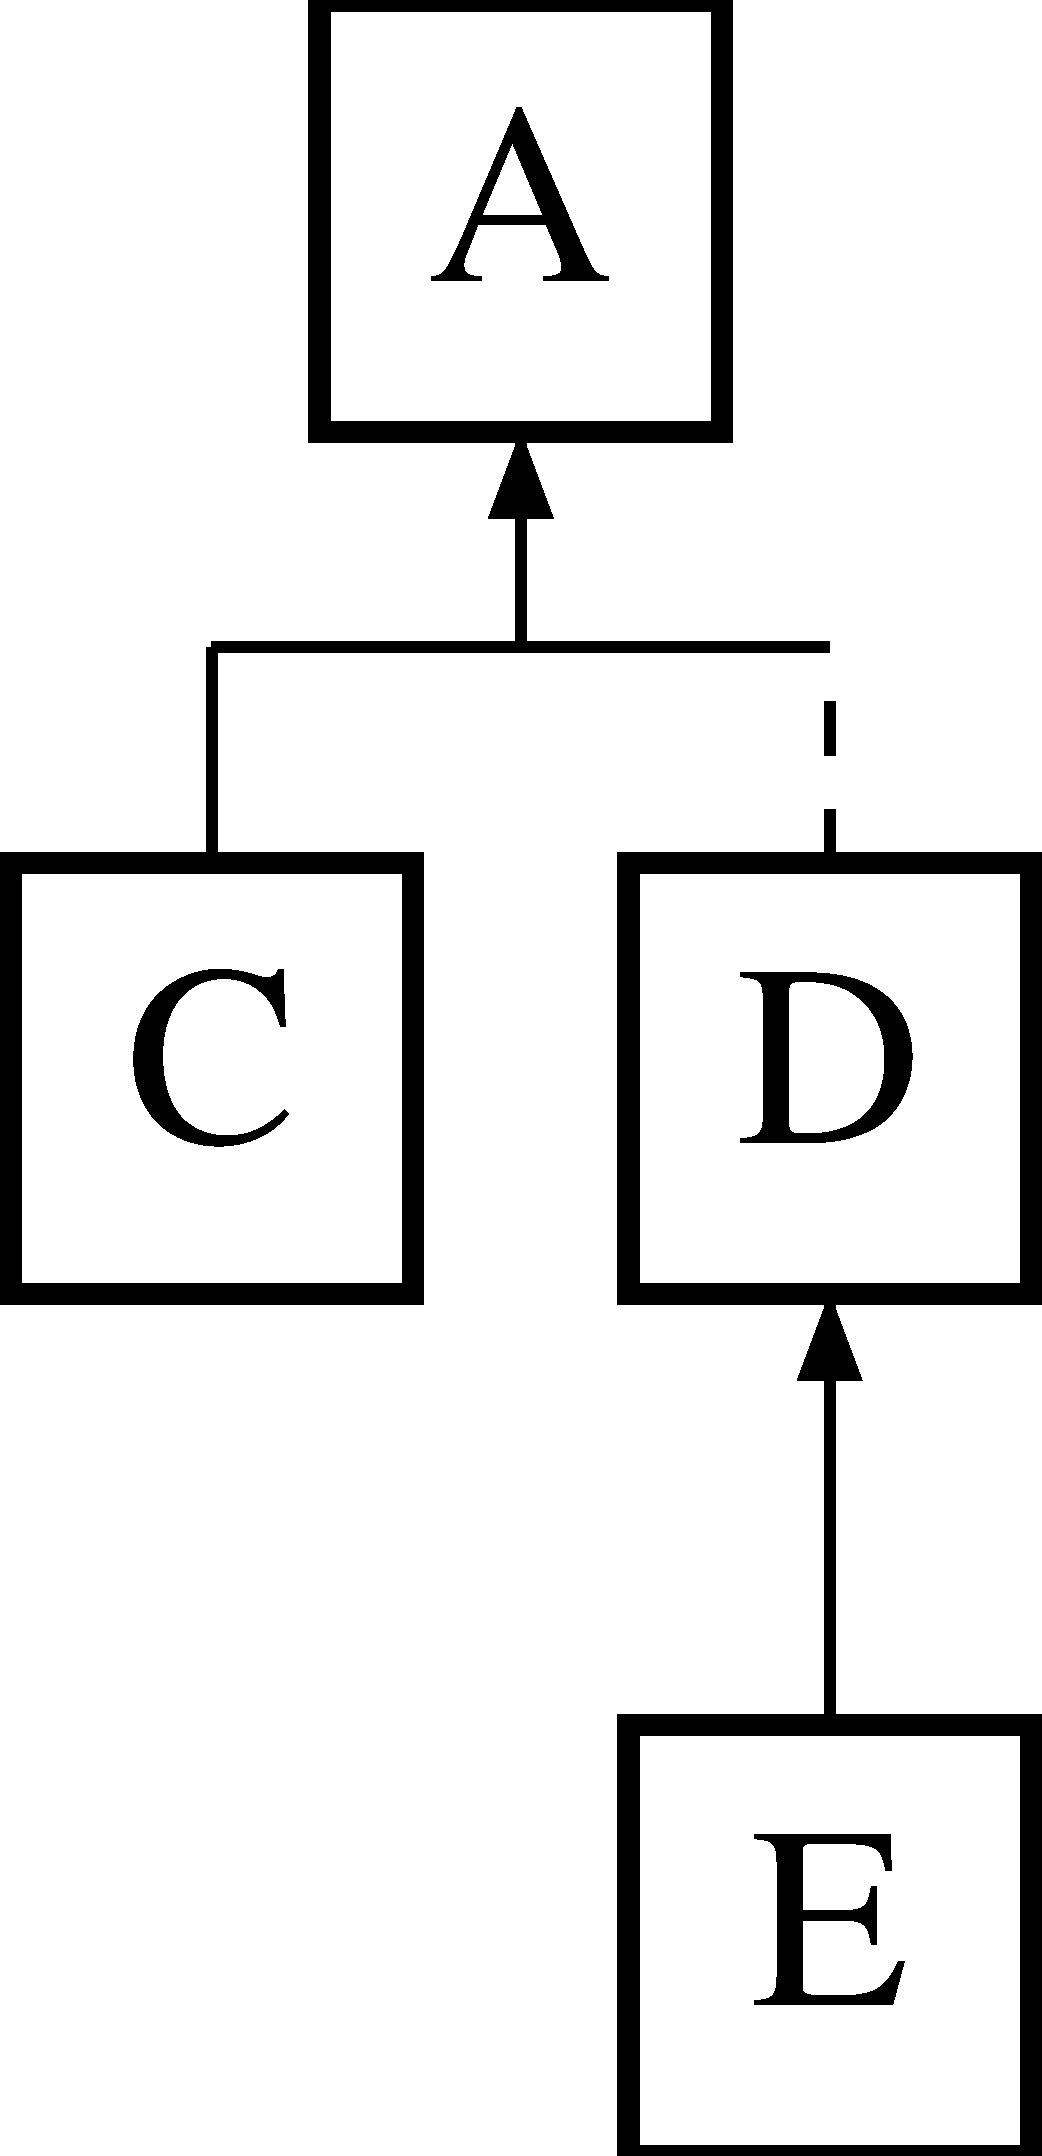
\includegraphics[height=3.000000cm]{class_a}
\end{center}
\end{figure}
\subsection*{Public Attributes}
\begin{DoxyCompactItemize}
\item 
\hypertarget{class_a_a086d3a4efc697dba0601b9fef3d082ad}{\hyperlink{class_a}{A} $\ast$ {\bfseries m\-\_\-self}}\label{class_a_a086d3a4efc697dba0601b9fef3d082ad}

\end{DoxyCompactItemize}


The documentation for this class was generated from the following file\-:\begin{DoxyCompactItemize}
\item 
diagrams\-\_\-a.\-h\end{DoxyCompactItemize}

\hypertarget{class_b}{\section{B Class Reference}
\label{class_b}\index{B@{B}}
}
Inheritance diagram for B\-:\begin{figure}[H]
\begin{center}
\leavevmode
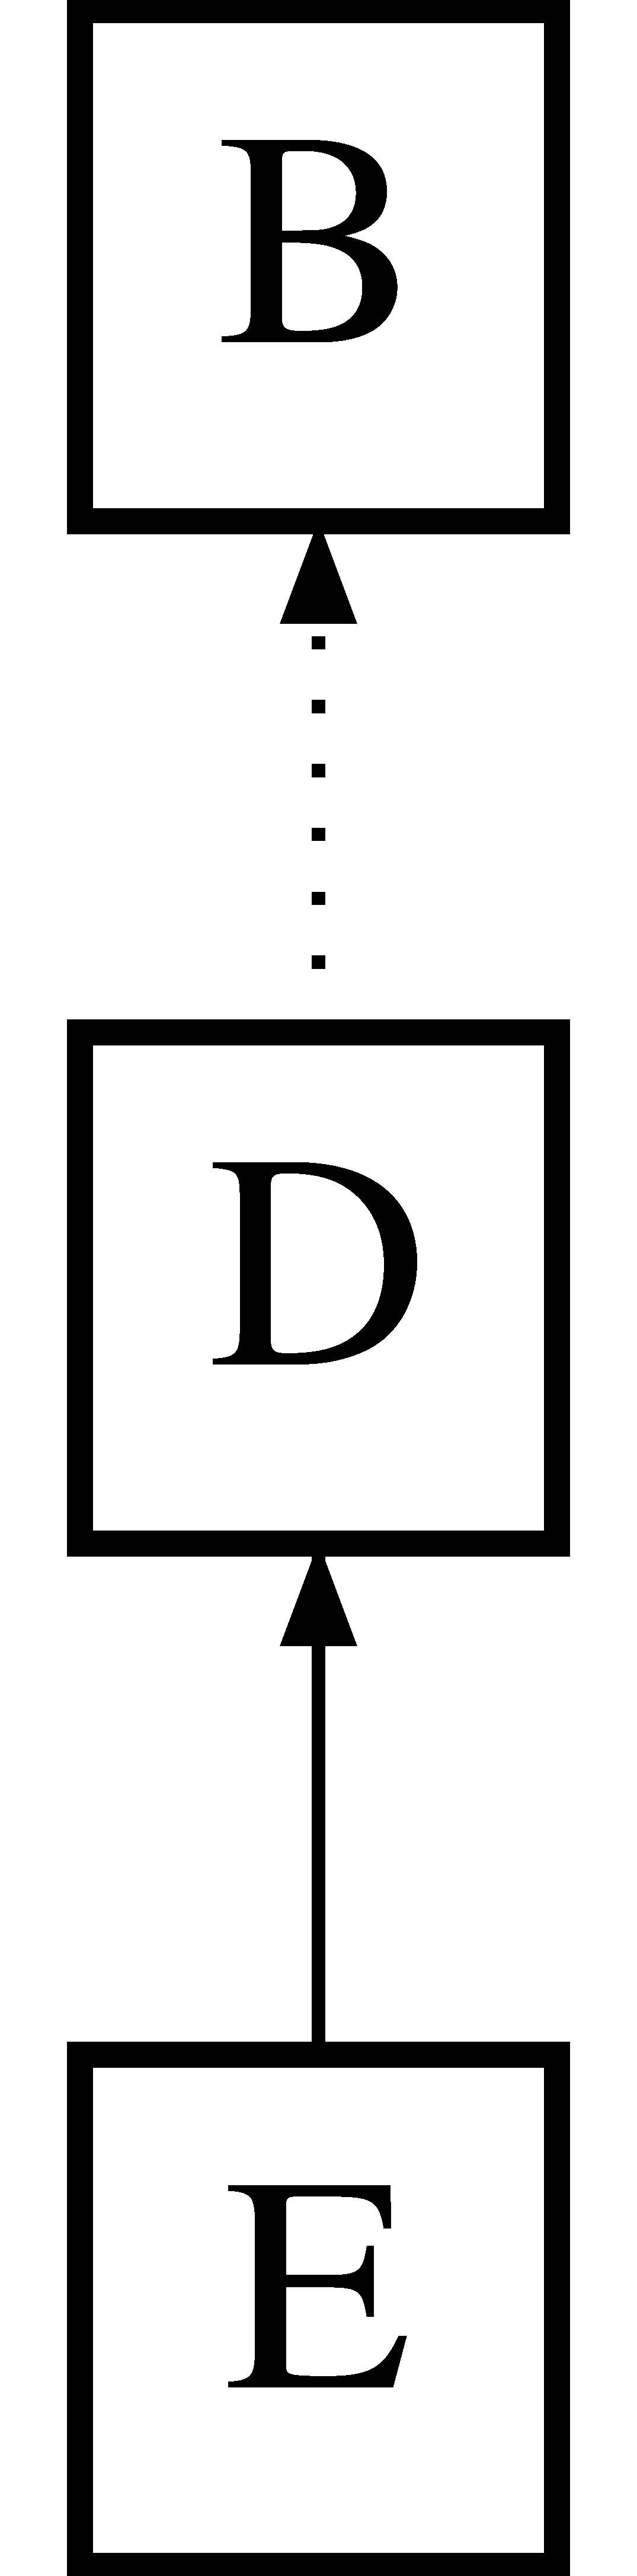
\includegraphics[height=3.000000cm]{class_b}
\end{center}
\end{figure}
\subsection*{Public Attributes}
\begin{DoxyCompactItemize}
\item 
\hypertarget{class_b_a26c70b64fe7cf17fcced7755ecff7537}{\hyperlink{class_a}{A} $\ast$ {\bfseries m\-\_\-a}}\label{class_b_a26c70b64fe7cf17fcced7755ecff7537}

\end{DoxyCompactItemize}


The documentation for this class was generated from the following file\-:\begin{DoxyCompactItemize}
\item 
diagrams\-\_\-b.\-h\end{DoxyCompactItemize}

\hypertarget{class_c}{\section{C Class Reference}
\label{class_c}\index{C@{C}}
}
Inheritance diagram for C\-:\begin{figure}[H]
\begin{center}
\leavevmode
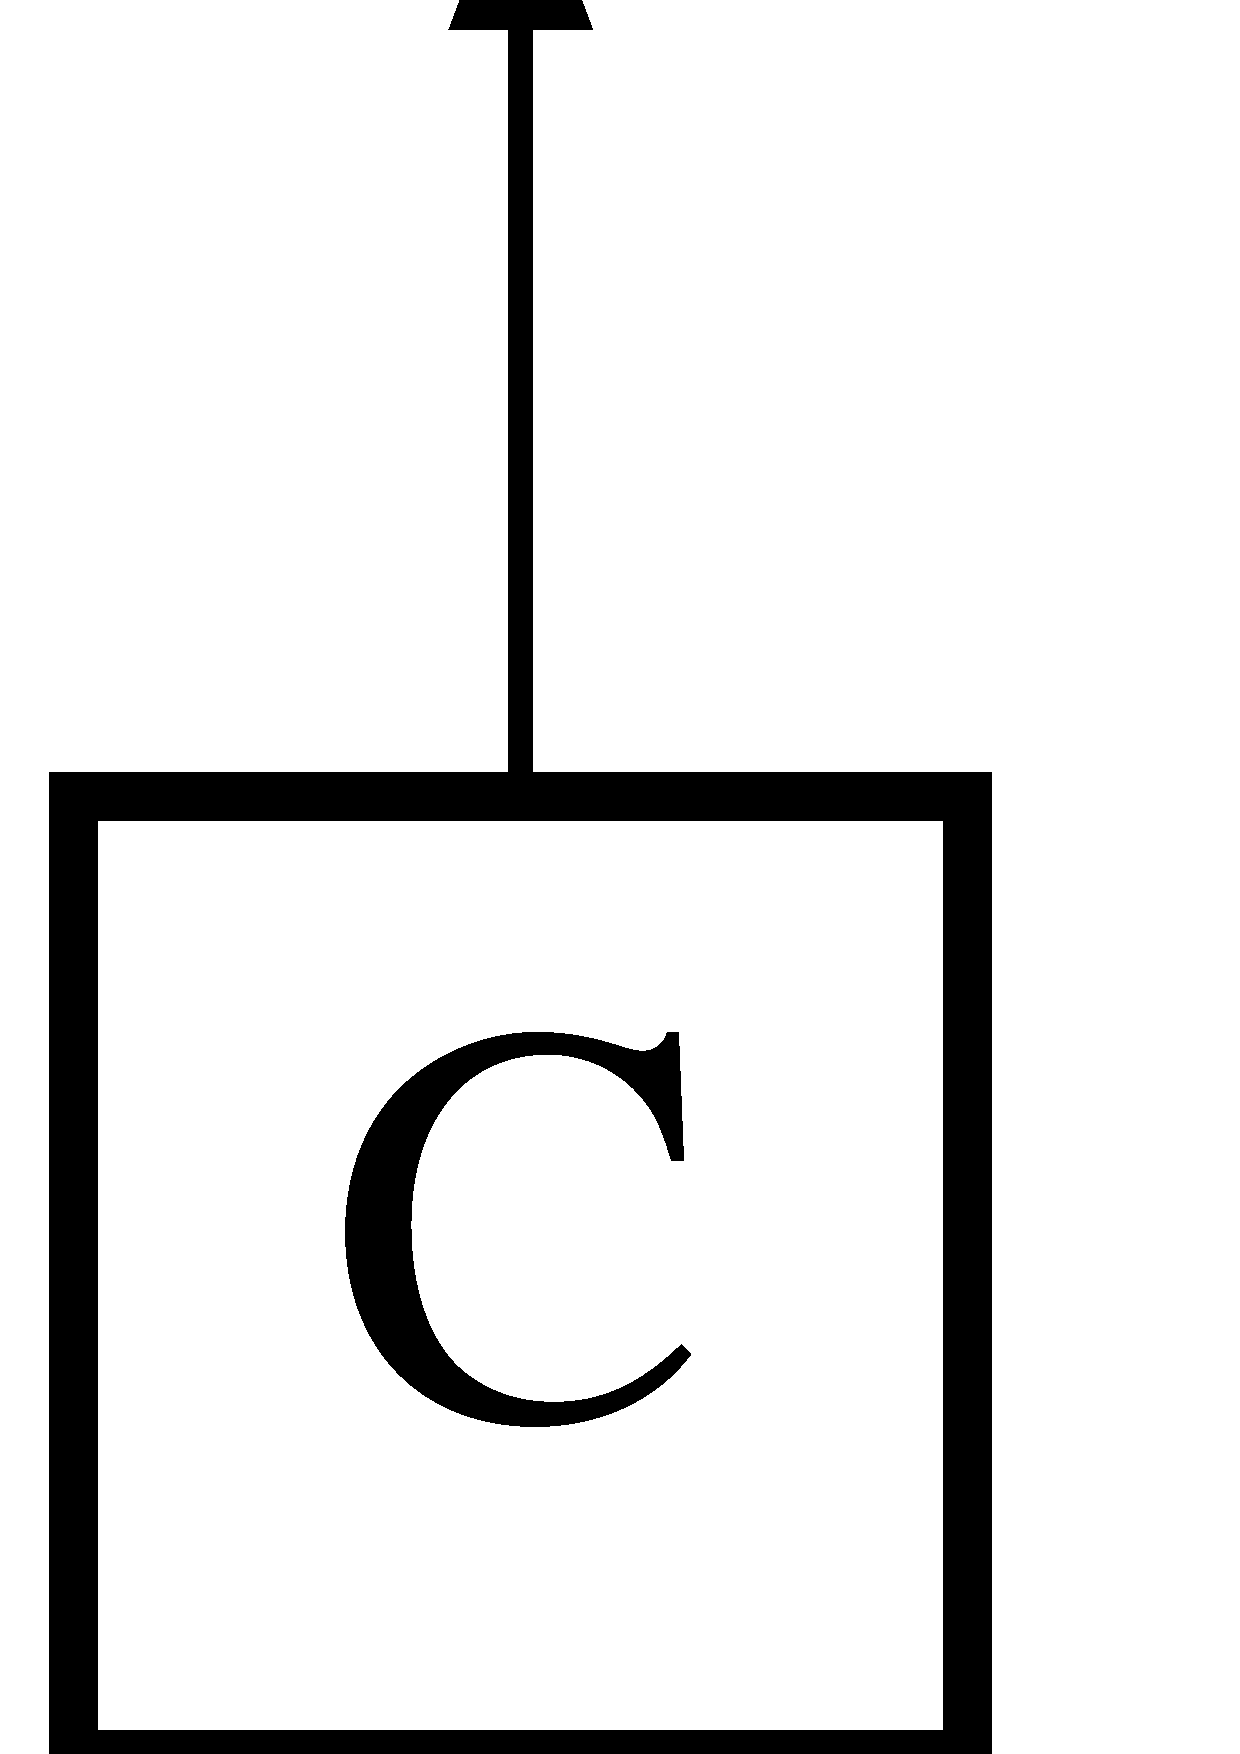
\includegraphics[height=2.000000cm]{class_c}
\end{center}
\end{figure}
\subsection*{Public Attributes}
\begin{DoxyCompactItemize}
\item 
\hypertarget{class_c_a4ef972d28b73ff78eba3ab4f54c3b449}{\hyperlink{class_d}{D} $\ast$ {\bfseries m\-\_\-d}}\label{class_c_a4ef972d28b73ff78eba3ab4f54c3b449}

\end{DoxyCompactItemize}


The documentation for this class was generated from the following file\-:\begin{DoxyCompactItemize}
\item 
diagrams\-\_\-c.\-h\end{DoxyCompactItemize}

\hypertarget{class_c1}{\section{C1 Class Reference}
\label{class_c1}\index{C1@{C1}}
}


class \hyperlink{class_c1}{C1} in group 1  




\subsection{Detailed Description}
class \hyperlink{class_c1}{C1} in group 1 

The documentation for this class was generated from the following file\-:\begin{DoxyCompactItemize}
\item 
\hyperlink{group_8cpp}{group.\-cpp}\end{DoxyCompactItemize}

\hypertarget{class_c2}{\section{C2 Class Reference}
\label{class_c2}\index{C2@{C2}}
}


class \hyperlink{class_c2}{C2} in group 1  




\subsection{Detailed Description}
class \hyperlink{class_c2}{C2} in group 1 

The documentation for this class was generated from the following file\-:\begin{DoxyCompactItemize}
\item 
\hyperlink{group_8cpp}{group.\-cpp}\end{DoxyCompactItemize}

\hypertarget{class_c3}{\section{C3 Class Reference}
\label{class_c3}\index{C3@{C3}}
}


class \hyperlink{class_c3}{C3} in group 2  




\subsection{Detailed Description}
class \hyperlink{class_c3}{C3} in group 2 

The documentation for this class was generated from the following file\-:\begin{DoxyCompactItemize}
\item 
\hyperlink{group_8cpp}{group.\-cpp}\end{DoxyCompactItemize}

\hypertarget{class_c4}{\section{C4 Class Reference}
\label{class_c4}\index{C4@{C4}}
}


class \hyperlink{class_c4}{C4} in group 2  




\subsection{Detailed Description}
class \hyperlink{class_c4}{C4} in group 2 

The documentation for this class was generated from the following file\-:\begin{DoxyCompactItemize}
\item 
\hyperlink{group_8cpp}{group.\-cpp}\end{DoxyCompactItemize}

\hypertarget{class_c5}{\section{C5 Class Reference}
\label{class_c5}\index{C5@{C5}}
}


class \hyperlink{class_c5}{C5} in \hyperlink{group__group3}{the third group}.  




\subsection{Detailed Description}
class \hyperlink{class_c5}{C5} in \hyperlink{group__group3}{the third group}. 

The documentation for this class was generated from the following file\-:\begin{DoxyCompactItemize}
\item 
\hyperlink{group_8cpp}{group.\-cpp}\end{DoxyCompactItemize}

\hypertarget{struct_car}{\section{Car Struct Reference}
\label{struct_car}\index{Car@{Car}}
}
Inheritance diagram for Car\-:\begin{figure}[H]
\begin{center}
\leavevmode
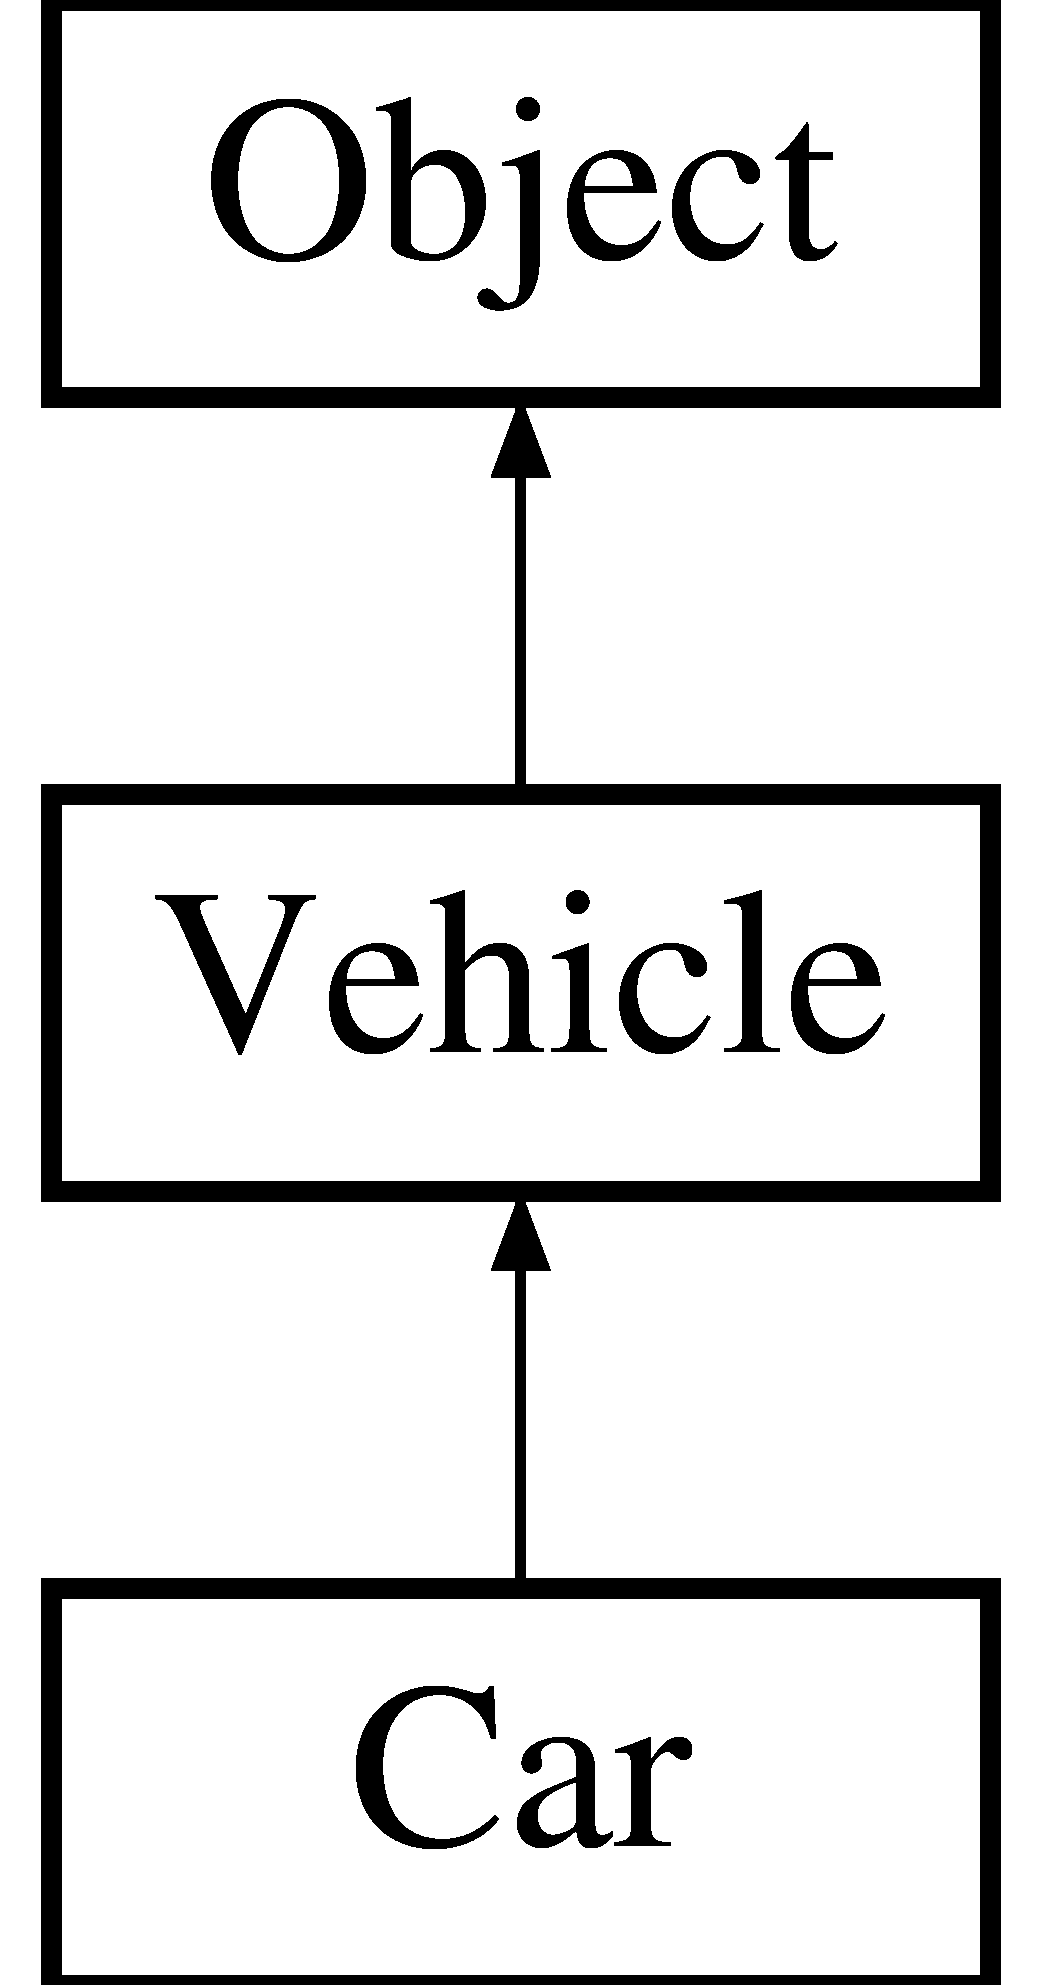
\includegraphics[height=3.000000cm]{struct_car}
\end{center}
\end{figure}
\subsection*{Protected Attributes}
\begin{DoxyCompactItemize}
\item 
\hypertarget{struct_car_ab8ff28306286da5a8b14fa9bdccaafaa}{\hyperlink{struct_vehicle}{Vehicle} \hyperlink{struct_car_ab8ff28306286da5a8b14fa9bdccaafaa}{base}}\label{struct_car_ab8ff28306286da5a8b14fa9bdccaafaa}

\begin{DoxyCompactList}\small\item\em Base class. \end{DoxyCompactList}\end{DoxyCompactItemize}
\subsection*{Additional Inherited Members}


\subsection{Detailed Description}
\hyperlink{struct_car}{Car} class. 

The documentation for this struct was generated from the following file\-:\begin{DoxyCompactItemize}
\item 
\hyperlink{manual_8c}{manual.\-c}\end{DoxyCompactItemize}

\hypertarget{struct_coord_struct}{\section{Coord\-Struct Struct Reference}
\label{struct_coord_struct}\index{Coord\-Struct@{Coord\-Struct}}
}
\subsection*{Public Attributes}
\begin{DoxyCompactItemize}
\item 
float \hyperlink{struct_coord_struct_a183d7226fc5a8470ce9b9f04f9cb69bb}{x}
\item 
float \hyperlink{struct_coord_struct_a1a5966a881bc3e76e9becf00639585ac}{y}
\end{DoxyCompactItemize}


\subsection{Detailed Description}
\hyperlink{class_a}{A} coordinate pair. 

\subsection{Member Data Documentation}
\hypertarget{struct_coord_struct_a183d7226fc5a8470ce9b9f04f9cb69bb}{\index{Coord\-Struct@{Coord\-Struct}!x@{x}}
\index{x@{x}!CoordStruct@{Coord\-Struct}}
\subsubsection[{x}]{\setlength{\rightskip}{0pt plus 5cm}float Coord\-Struct\-::x}}\label{struct_coord_struct_a183d7226fc5a8470ce9b9f04f9cb69bb}
The x coordinate \hypertarget{struct_coord_struct_a1a5966a881bc3e76e9becf00639585ac}{\index{Coord\-Struct@{Coord\-Struct}!y@{y}}
\index{y@{y}!CoordStruct@{Coord\-Struct}}
\subsubsection[{y}]{\setlength{\rightskip}{0pt plus 5cm}float Coord\-Struct\-::y}}\label{struct_coord_struct_a1a5966a881bc3e76e9becf00639585ac}
The y coordinate 

The documentation for this struct was generated from the following file\-:\begin{DoxyCompactItemize}
\item 
\hyperlink{restypedef_8cpp}{restypedef.\-cpp}\end{DoxyCompactItemize}

\hypertarget{class_d}{\section{D Class Reference}
\label{class_d}\index{D@{D}}
}
Inheritance diagram for D\-:\begin{figure}[H]
\begin{center}
\leavevmode
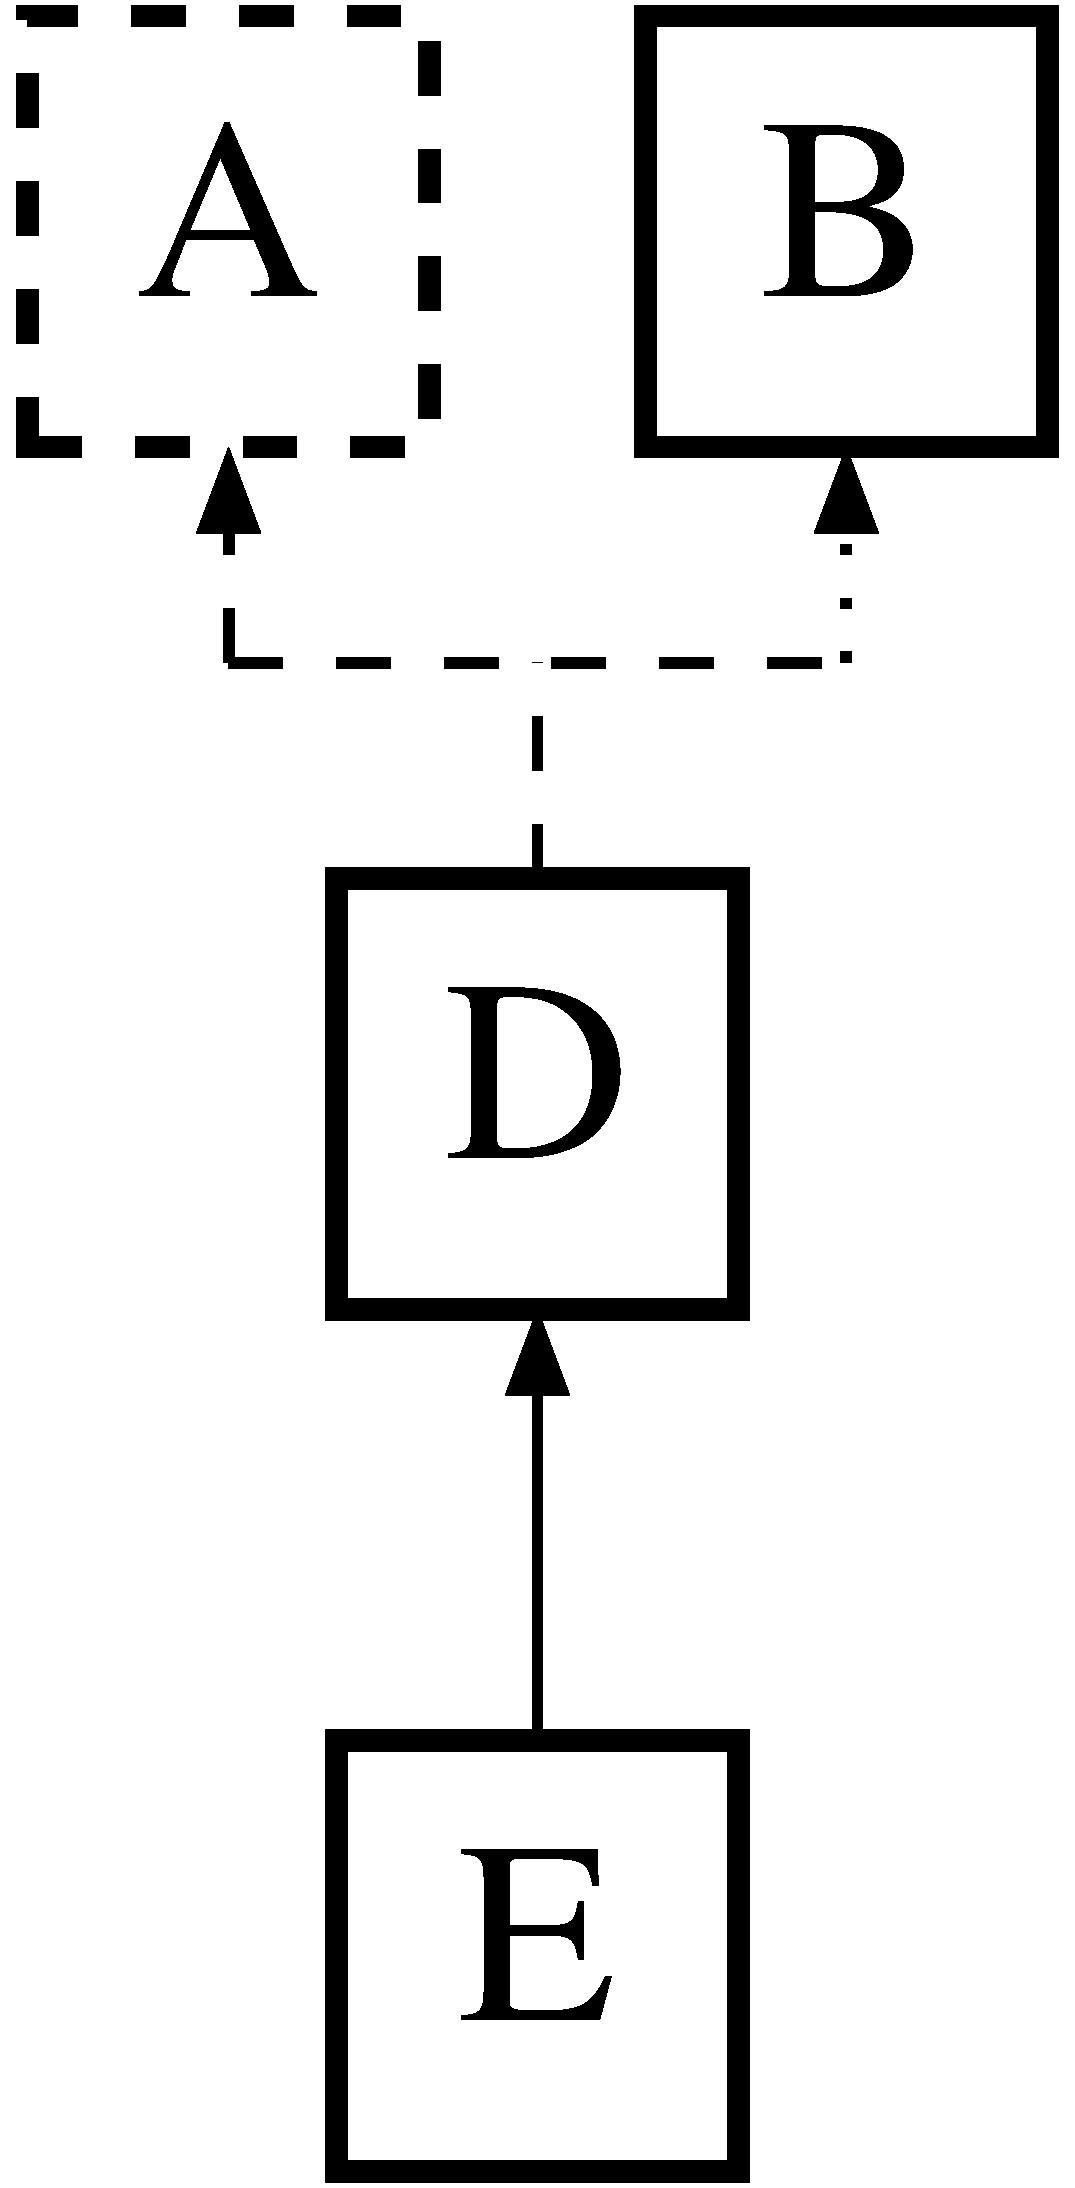
\includegraphics[height=3.000000cm]{class_d}
\end{center}
\end{figure}
\subsection*{Public Attributes}
\begin{DoxyCompactItemize}
\item 
\hypertarget{class_d_a9d877c7aa092f423f2a073f3c62fef9c}{\hyperlink{class_c}{C} {\bfseries m\-\_\-c}}\label{class_d_a9d877c7aa092f423f2a073f3c62fef9c}

\end{DoxyCompactItemize}
\subsection*{Additional Inherited Members}


The documentation for this class was generated from the following file\-:\begin{DoxyCompactItemize}
\item 
diagrams\-\_\-d.\-h\end{DoxyCompactItemize}

\hypertarget{class_e}{\section{E Class Reference}
\label{class_e}\index{E@{E}}
}
Inheritance diagram for E\-:\begin{figure}[H]
\begin{center}
\leavevmode
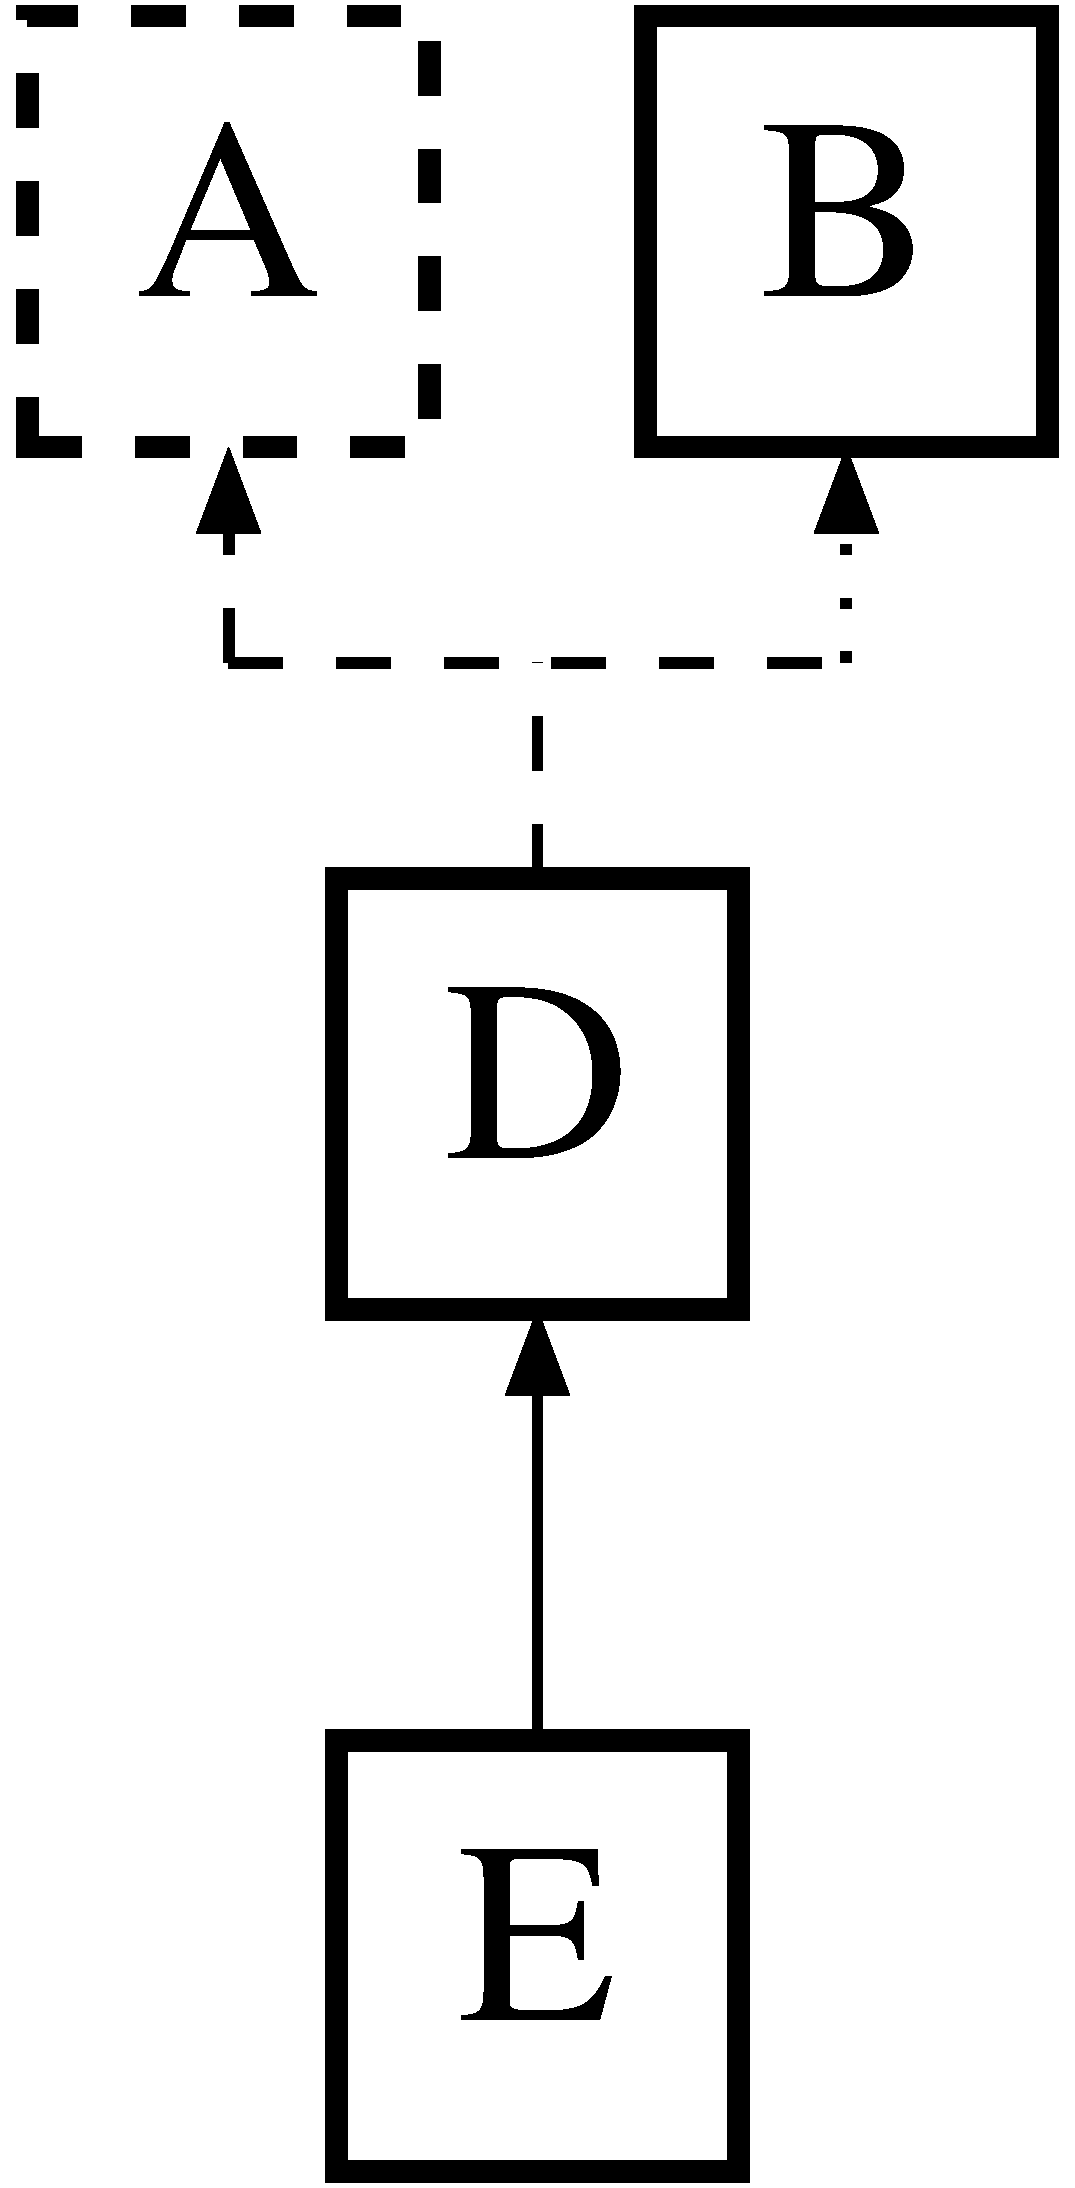
\includegraphics[height=3.000000cm]{class_e}
\end{center}
\end{figure}
\subsection*{Additional Inherited Members}


The documentation for this class was generated from the following file\-:\begin{DoxyCompactItemize}
\item 
diagrams\-\_\-e.\-h\end{DoxyCompactItemize}

\hypertarget{classns_1_1itcl__class}{\section{ns\-:\-:itcl\-\_\-class Class Reference}
\label{classns_1_1itcl__class}\index{ns\-::itcl\-\_\-class@{ns\-::itcl\-\_\-class}}
}
\subsection*{Public Member Functions}
\begin{DoxyCompactItemize}
\item 
\hyperlink{classns_1_1itcl__class_a8ba2ba9d7bcb63b99a765e8f6003134b}{constructor} args
\item 
\hyperlink{classns_1_1itcl__class_ac72f3174993656391f9b54487aa4795e}{destructor}
\item 
\hyperlink{classns_1_1itcl__class_abc59160f823f3a6ec8c292c034aedbc3}{itcl\-\_\-method\-\_\-x} arg
\item 
\hyperlink{classns_1_1itcl__class_a092d0f8ed4796902e41fbeb1dfed82f1}{itcl\-\_\-method\-\_\-y} arg
\item 
\hyperlink{classns_1_1itcl__class_a13a383c766e489814960345540106cc1}{itcl\-\_\-method\-\_\-z} arg
\item 
\hypertarget{classns_1_1itcl__class_aad1f81467f2fca0dc02e527e786513a4}{{\bfseries itcl\-\_\-method\-\_\-x} argx}\label{classns_1_1itcl__class_aad1f81467f2fca0dc02e527e786513a4}

\end{DoxyCompactItemize}
\subsection*{Static Public Attributes}
\begin{DoxyCompactItemize}
\item 
\hyperlink{classns_1_1itcl__class_a8df46696ce554fed04d170932260fbb8}{itcl\-\_\-\-Var}
\item 
\hypertarget{classns_1_1itcl__class_abaf3c744194c1b3ae68fb0ba70d8786e}{{\bfseries itcl\-\_\-var2}}\label{classns_1_1itcl__class_abaf3c744194c1b3ae68fb0ba70d8786e}

\end{DoxyCompactItemize}
\subsection*{Static Protected Attributes}
\begin{DoxyCompactItemize}
\item 
\hypertarget{classns_1_1itcl__class_ae515e43ca6bb755d116416f94a13d344}{\hyperlink{classns_1_1itcl__class_ae515e43ca6bb755d116416f94a13d344}{itcl\-\_\-var1}}\label{classns_1_1itcl__class_ae515e43ca6bb755d116416f94a13d344}

\begin{DoxyCompactList}\small\item\em Documented itcl var {\ttfamily itcl\-\_\-var1} . \end{DoxyCompactList}\end{DoxyCompactItemize}


\subsection{Detailed Description}
Documented itcl class {\ttfamily \hyperlink{classns_1_1itcl__class}{itcl\-\_\-class}} . 

\subsection{Constructor \& Destructor Documentation}
\hypertarget{classns_1_1itcl__class_a8ba2ba9d7bcb63b99a765e8f6003134b}{\index{ns\-::itcl\-\_\-class@{ns\-::itcl\-\_\-class}!constructor@{constructor}}
\index{constructor@{constructor}!ns::itcl_class@{ns\-::itcl\-\_\-class}}
\subsubsection[{constructor}]{\setlength{\rightskip}{0pt plus 5cm}ns\-::itcl\-\_\-class\-::constructor {args }
}}\label{classns_1_1itcl__class_a8ba2ba9d7bcb63b99a765e8f6003134b}
Create object. \hypertarget{classns_1_1itcl__class_ac72f3174993656391f9b54487aa4795e}{\index{ns\-::itcl\-\_\-class@{ns\-::itcl\-\_\-class}!destructor@{destructor}}
\index{destructor@{destructor}!ns::itcl_class@{ns\-::itcl\-\_\-class}}
\subsubsection[{destructor}]{\setlength{\rightskip}{0pt plus 5cm}ns\-::itcl\-\_\-class\-::destructor {}
}}\label{classns_1_1itcl__class_ac72f3174993656391f9b54487aa4795e}
Destroy object. 

\subsection{Member Function Documentation}
\hypertarget{classns_1_1itcl__class_abc59160f823f3a6ec8c292c034aedbc3}{\index{ns\-::itcl\-\_\-class@{ns\-::itcl\-\_\-class}!itcl\-\_\-method\-\_\-x@{itcl\-\_\-method\-\_\-x}}
\index{itcl\-\_\-method\-\_\-x@{itcl\-\_\-method\-\_\-x}!ns::itcl_class@{ns\-::itcl\-\_\-class}}
\subsubsection[{itcl\-\_\-method\-\_\-x}]{\setlength{\rightskip}{0pt plus 5cm}ns\-::itcl\-\_\-class\-::itcl\-\_\-method\-\_\-x {arg }
}}\label{classns_1_1itcl__class_abc59160f823f3a6ec8c292c034aedbc3}
Documented itcl method {\ttfamily itcl\-\_\-method\-\_\-x} . param\mbox{[}in\mbox{]} arg Argument \hypertarget{classns_1_1itcl__class_a092d0f8ed4796902e41fbeb1dfed82f1}{\index{ns\-::itcl\-\_\-class@{ns\-::itcl\-\_\-class}!itcl\-\_\-method\-\_\-y@{itcl\-\_\-method\-\_\-y}}
\index{itcl\-\_\-method\-\_\-y@{itcl\-\_\-method\-\_\-y}!ns::itcl_class@{ns\-::itcl\-\_\-class}}
\subsubsection[{itcl\-\_\-method\-\_\-y}]{\setlength{\rightskip}{0pt plus 5cm}ns\-::itcl\-\_\-class\-::itcl\-\_\-method\-\_\-y {arg }
}}\label{classns_1_1itcl__class_a092d0f8ed4796902e41fbeb1dfed82f1}
Documented itcl method {\ttfamily itcl\-\_\-method\-\_\-y} . param\mbox{[}in\mbox{]} arg Argument \hypertarget{classns_1_1itcl__class_a13a383c766e489814960345540106cc1}{\index{ns\-::itcl\-\_\-class@{ns\-::itcl\-\_\-class}!itcl\-\_\-method\-\_\-z@{itcl\-\_\-method\-\_\-z}}
\index{itcl\-\_\-method\-\_\-z@{itcl\-\_\-method\-\_\-z}!ns::itcl_class@{ns\-::itcl\-\_\-class}}
\subsubsection[{itcl\-\_\-method\-\_\-z}]{\setlength{\rightskip}{0pt plus 5cm}ns\-::itcl\-\_\-class\-::itcl\-\_\-method\-\_\-z {arg }
}}\label{classns_1_1itcl__class_a13a383c766e489814960345540106cc1}
Documented itcl method {\ttfamily itcl\-\_\-method\-\_\-z} . param\mbox{[}in\mbox{]} arg Argument 

\subsection{Member Data Documentation}
\hypertarget{classns_1_1itcl__class_a8df46696ce554fed04d170932260fbb8}{\index{ns\-::itcl\-\_\-class@{ns\-::itcl\-\_\-class}!itcl\-\_\-\-Var@{itcl\-\_\-\-Var}}
\index{itcl\-\_\-\-Var@{itcl\-\_\-\-Var}!ns::itcl_class@{ns\-::itcl\-\_\-class}}
\subsubsection[{itcl\-\_\-\-Var}]{\setlength{\rightskip}{0pt plus 5cm}ns\-::itcl\-\_\-class\-::itcl\-\_\-\-Var\hspace{0.3cm}{\ttfamily [static]}}}\label{classns_1_1itcl__class_a8df46696ce554fed04d170932260fbb8}
Documented common itcl var {\ttfamily itcl\-\_\-\-Var} . 

The documentation for this class was generated from the following file\-:\begin{DoxyCompactItemize}
\item 
\hyperlink{tclexample_8tcl}{tclexample.\-tcl}\end{DoxyCompactItemize}

\hypertarget{classmux__using__with}{\section{mux\-\_\-using\-\_\-with Entity Reference}
\label{classmux__using__with}\index{mux\-\_\-using\-\_\-with@{mux\-\_\-using\-\_\-with}}
}


Mux entity brief description.  


\subsection*{Ports}
 \begin{DoxyCompactItemize}
\item 
\hyperlink{classmux__using__with_af60b470af850edfe2a766ef15ffcc7c1}{din\-\_\-0}  {\bfseries {\bfseries \textcolor{vhdlkeyword}{in}\textcolor{vhdlchar}{ }}} {\bfseries \textcolor{comment}{std\-\_\-logic}\textcolor{vhdlchar}{ }} 
\begin{DoxyCompactList}\small\item\em Mux first input. \end{DoxyCompactList}\item 
\hypertarget{classmux__using__with_a45a6e584caaf4eb967f79e90560e13a5}{\hyperlink{classmux__using__with_a45a6e584caaf4eb967f79e90560e13a5}{din\-\_\-1}  {\bfseries {\bfseries \textcolor{vhdlkeyword}{in}\textcolor{vhdlchar}{ }}} {\bfseries \textcolor{comment}{std\-\_\-logic}\textcolor{vhdlchar}{ }} }\label{classmux__using__with_a45a6e584caaf4eb967f79e90560e13a5}

\begin{DoxyCompactList}\small\item\em Mux Second input. \end{DoxyCompactList}\item 
\hypertarget{classmux__using__with_afdf90ff4b63a502f4a623b0afbda6d80}{\hyperlink{classmux__using__with_afdf90ff4b63a502f4a623b0afbda6d80}{sel}  {\bfseries {\bfseries \textcolor{vhdlkeyword}{in}\textcolor{vhdlchar}{ }}} {\bfseries \textcolor{comment}{std\-\_\-logic}\textcolor{vhdlchar}{ }} }\label{classmux__using__with_afdf90ff4b63a502f4a623b0afbda6d80}

\begin{DoxyCompactList}\small\item\em Select input. \end{DoxyCompactList}\item 
\hypertarget{classmux__using__with_a22f89b66523a35bf7f80cac1d166fe0f}{\hyperlink{classmux__using__with_a22f89b66523a35bf7f80cac1d166fe0f}{mux\-\_\-out}  {\bfseries {\bfseries \textcolor{vhdlkeyword}{out}\textcolor{vhdlchar}{ }}} {\bfseries \textcolor{comment}{std\-\_\-logic}\textcolor{vhdlchar}{ }} }\label{classmux__using__with_a22f89b66523a35bf7f80cac1d166fe0f}

\begin{DoxyCompactList}\small\item\em Mux output. \end{DoxyCompactList}\end{DoxyCompactItemize}


\subsection{Detailed Description}
Mux entity brief description. 

\subsection{Member Data Documentation}
\hypertarget{classmux__using__with_af60b470af850edfe2a766ef15ffcc7c1}{\index{mux\-\_\-using\-\_\-with@{mux\-\_\-using\-\_\-with}!din\-\_\-0@{din\-\_\-0}}
\index{din\-\_\-0@{din\-\_\-0}!mux_using_with@{mux\-\_\-using\-\_\-with}}
\subsubsection[{din\-\_\-0}]{\setlength{\rightskip}{0pt plus 5cm}{\bf din\-\_\-0} {\bfseries \textcolor{vhdlkeyword}{in}\textcolor{vhdlchar}{ }} {\bfseries \textcolor{comment}{std\-\_\-logic}\textcolor{vhdlchar}{ }} \hspace{0.3cm}{\ttfamily [Port]}}}\label{classmux__using__with_af60b470af850edfe2a766ef15ffcc7c1}


Mux first input. 

Detailed description of this mux design element. 

The documentation for this class was generated from the following file\-:\begin{DoxyCompactItemize}
\item 
\hyperlink{mux_8vhdl}{mux.\-vhdl}\end{DoxyCompactItemize}

\hypertarget{struct_object}{\section{Object Struct Reference}
\label{struct_object}\index{Object@{Object}}
}
Inheritance diagram for Object\-:\begin{figure}[H]
\begin{center}
\leavevmode
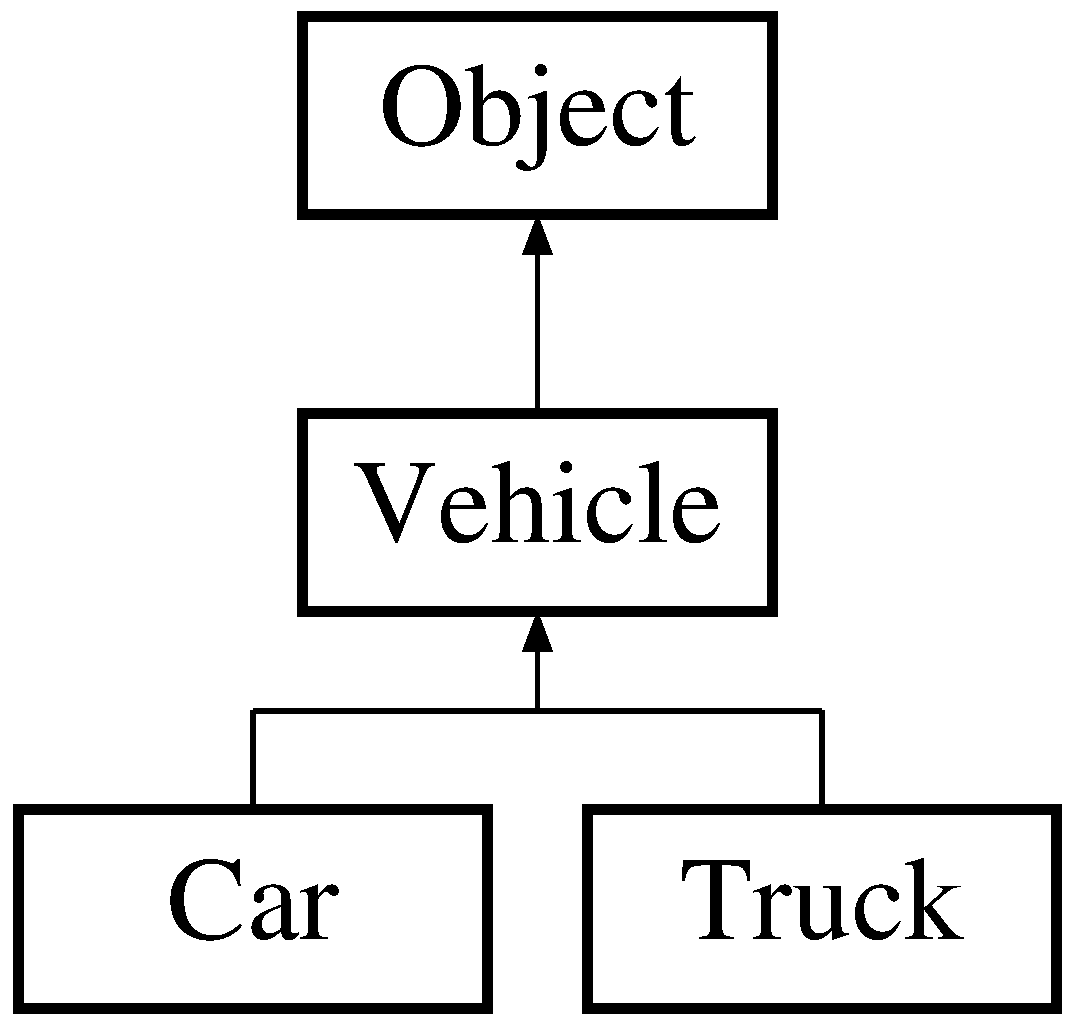
\includegraphics[height=3.000000cm]{struct_object}
\end{center}
\end{figure}
\subsection*{Public Member Functions}
\begin{DoxyCompactItemize}
\item 
static \hyperlink{struct_object}{Object} $\ast$ \hyperlink{struct_object_a71225073d06a793b9a6ea9263ed37b12}{obj\-Ref} (\hyperlink{struct_object}{Object} $\ast$obj)
\item 
static \hyperlink{struct_object}{Object} $\ast$ \hyperlink{struct_object_a924ee0cecc906d148022b3f0d6325cfb}{obj\-Unref} (\hyperlink{struct_object}{Object} $\ast$obj)
\end{DoxyCompactItemize}


\subsection{Detailed Description}
Base object class. 

\subsection{Member Function Documentation}
\hypertarget{struct_object_a71225073d06a793b9a6ea9263ed37b12}{\index{Object@{Object}!obj\-Ref@{obj\-Ref}}
\index{obj\-Ref@{obj\-Ref}!Object@{Object}}
\subsubsection[{obj\-Ref}]{\setlength{\rightskip}{0pt plus 5cm}static {\bf Object} $\ast$ obj\-Ref (
\begin{DoxyParamCaption}
\item[{{\bf Object} $\ast$}]{obj}
\end{DoxyParamCaption}
)}}\label{struct_object_a71225073d06a793b9a6ea9263ed37b12}
Increments object reference count by one. \hypertarget{struct_object_a924ee0cecc906d148022b3f0d6325cfb}{\index{Object@{Object}!obj\-Unref@{obj\-Unref}}
\index{obj\-Unref@{obj\-Unref}!Object@{Object}}
\subsubsection[{obj\-Unref}]{\setlength{\rightskip}{0pt plus 5cm}static {\bf Object} $\ast$ obj\-Unref (
\begin{DoxyParamCaption}
\item[{{\bf Object} $\ast$}]{obj}
\end{DoxyParamCaption}
)}}\label{struct_object_a924ee0cecc906d148022b3f0d6325cfb}
Decrements object reference count by one. 

The documentation for this struct was generated from the following file\-:\begin{DoxyCompactItemize}
\item 
\hyperlink{manual_8c}{manual.\-c}\end{DoxyCompactItemize}

\hypertarget{classns_1_1oo__class}{\section{ns\-:\-:oo\-\_\-class Class Reference}
\label{classns_1_1oo__class}\index{ns\-::oo\-\_\-class@{ns\-::oo\-\_\-class}}
}
\subsection*{Public Member Functions}
\begin{DoxyCompactItemize}
\item 
\hyperlink{classns_1_1oo__class_aa26b64151d4b4b0e8b4977aae7048f9b}{constructor} args
\item 
\hyperlink{classns_1_1oo__class_af148cfc1c090a05986c68ac9452a510a}{destructor}
\item 
\hyperlink{classns_1_1oo__class_a8a3cfbae3b3fca463f08adb9174a5fe8}{oo\-\_\-method\-\_\-z} arg
\end{DoxyCompactItemize}
\subsection*{Static Public Attributes}
\begin{DoxyCompactItemize}
\item 
\hyperlink{classns_1_1oo__class_a741f11f4a2db3876205658d4a9a279ba}{oo\-\_\-var}
\item 
\hyperlink{classns_1_1oo__class_af46293ede16067c38ca2901416cad8ee}{oo\-\_\-var\-\_\-out}
\end{DoxyCompactItemize}
\subsection*{Protected Member Functions}
\begin{DoxyCompactItemize}
\item 
\hyperlink{classns_1_1oo__class_ad07feb192f34010ed66d123338c7acdd}{oo\-\_\-method\-\_\-y} arg
\end{DoxyCompactItemize}


\subsection{Detailed Description}
Documented oo class {\ttfamily \hyperlink{classns_1_1oo__class}{oo\-\_\-class}} . 

\subsection{Constructor \& Destructor Documentation}
\hypertarget{classns_1_1oo__class_aa26b64151d4b4b0e8b4977aae7048f9b}{\index{ns\-::oo\-\_\-class@{ns\-::oo\-\_\-class}!constructor@{constructor}}
\index{constructor@{constructor}!ns::oo_class@{ns\-::oo\-\_\-class}}
\subsubsection[{constructor}]{\setlength{\rightskip}{0pt plus 5cm}ns\-::oo\-\_\-class\-::constructor {args }
}}\label{classns_1_1oo__class_aa26b64151d4b4b0e8b4977aae7048f9b}
Create object. Configure with args \hypertarget{classns_1_1oo__class_af148cfc1c090a05986c68ac9452a510a}{\index{ns\-::oo\-\_\-class@{ns\-::oo\-\_\-class}!destructor@{destructor}}
\index{destructor@{destructor}!ns::oo_class@{ns\-::oo\-\_\-class}}
\subsubsection[{destructor}]{\setlength{\rightskip}{0pt plus 5cm}ns\-::oo\-\_\-class\-::destructor {}
}}\label{classns_1_1oo__class_af148cfc1c090a05986c68ac9452a510a}
Destroy object. Exit. 

\subsection{Member Function Documentation}
\hypertarget{classns_1_1oo__class_ad07feb192f34010ed66d123338c7acdd}{\index{ns\-::oo\-\_\-class@{ns\-::oo\-\_\-class}!oo\-\_\-method\-\_\-y@{oo\-\_\-method\-\_\-y}}
\index{oo\-\_\-method\-\_\-y@{oo\-\_\-method\-\_\-y}!ns::oo_class@{ns\-::oo\-\_\-class}}
\subsubsection[{oo\-\_\-method\-\_\-y}]{\setlength{\rightskip}{0pt plus 5cm}ns\-::oo\-\_\-class\-::oo\-\_\-method\-\_\-y {arg }
\hspace{0.3cm}{\ttfamily [protected]}}}\label{classns_1_1oo__class_ad07feb192f34010ed66d123338c7acdd}
Documented oo method {\ttfamily oo\-\_\-method\-\_\-y} . param\mbox{[}in\mbox{]} arg Argument \hypertarget{classns_1_1oo__class_a8a3cfbae3b3fca463f08adb9174a5fe8}{\index{ns\-::oo\-\_\-class@{ns\-::oo\-\_\-class}!oo\-\_\-method\-\_\-z@{oo\-\_\-method\-\_\-z}}
\index{oo\-\_\-method\-\_\-z@{oo\-\_\-method\-\_\-z}!ns::oo_class@{ns\-::oo\-\_\-class}}
\subsubsection[{oo\-\_\-method\-\_\-z}]{\setlength{\rightskip}{0pt plus 5cm}ns\-::oo\-\_\-class\-::oo\-\_\-method\-\_\-z {arg }
}}\label{classns_1_1oo__class_a8a3cfbae3b3fca463f08adb9174a5fe8}
Documented oo method {\ttfamily oo\-\_\-method\-\_\-z} . param\mbox{[}in\mbox{]} arg Argument 

\subsection{Member Data Documentation}
\hypertarget{classns_1_1oo__class_a741f11f4a2db3876205658d4a9a279ba}{\index{ns\-::oo\-\_\-class@{ns\-::oo\-\_\-class}!oo\-\_\-var@{oo\-\_\-var}}
\index{oo\-\_\-var@{oo\-\_\-var}!ns::oo_class@{ns\-::oo\-\_\-class}}
\subsubsection[{oo\-\_\-var}]{\setlength{\rightskip}{0pt plus 5cm}ns\-::oo\-\_\-class\-::oo\-\_\-var\hspace{0.3cm}{\ttfamily [static]}}}\label{classns_1_1oo__class_a741f11f4a2db3876205658d4a9a279ba}
Documented oo var {\ttfamily oo\-\_\-var} . Defined inside class \hypertarget{classns_1_1oo__class_af46293ede16067c38ca2901416cad8ee}{\index{ns\-::oo\-\_\-class@{ns\-::oo\-\_\-class}!oo\-\_\-var\-\_\-out@{oo\-\_\-var\-\_\-out}}
\index{oo\-\_\-var\-\_\-out@{oo\-\_\-var\-\_\-out}!ns::oo_class@{ns\-::oo\-\_\-class}}
\subsubsection[{oo\-\_\-var\-\_\-out}]{\setlength{\rightskip}{0pt plus 5cm}ns\-::oo\-\_\-class\-::oo\-\_\-var\-\_\-out\hspace{0.3cm}{\ttfamily [static]}}}\label{classns_1_1oo__class_af46293ede16067c38ca2901416cad8ee}
Outside defined variable {\ttfamily oo\-\_\-var\-\_\-out} . Inside \hyperlink{classns_1_1oo__class}{oo\-\_\-class} 

The documentation for this class was generated from the following file\-:\begin{DoxyCompactItemize}
\item 
\hyperlink{tclexample_8tcl}{tclexample.\-tcl}\end{DoxyCompactItemize}

\hypertarget{classdocstring_1_1_py_class}{\section{docstring.\-Py\-Class Class Reference}
\label{classdocstring_1_1_py_class}\index{docstring.\-Py\-Class@{docstring.\-Py\-Class}}
}
\subsection*{Public Member Functions}
\begin{DoxyCompactItemize}
\item 
def \hyperlink{classdocstring_1_1_py_class_ab9371d84572f9597933e59cb8b182c03}{\-\_\-\-\_\-init\-\_\-\-\_\-}
\item 
def \hyperlink{classdocstring_1_1_py_class_af76b8e03a20349e4d467aa37e65035bc}{Py\-Method}
\end{DoxyCompactItemize}


\subsection{Detailed Description}
\begin{DoxyVerb}Documentation for a class.

More details.
\end{DoxyVerb}
 

\subsection{Constructor \& Destructor Documentation}
\hypertarget{classdocstring_1_1_py_class_ab9371d84572f9597933e59cb8b182c03}{\index{docstring\-::\-Py\-Class@{docstring\-::\-Py\-Class}!\-\_\-\-\_\-init\-\_\-\-\_\-@{\-\_\-\-\_\-init\-\_\-\-\_\-}}
\index{\-\_\-\-\_\-init\-\_\-\-\_\-@{\-\_\-\-\_\-init\-\_\-\-\_\-}!docstring::PyClass@{docstring\-::\-Py\-Class}}
\subsubsection[{\-\_\-\-\_\-init\-\_\-\-\_\-}]{\setlength{\rightskip}{0pt plus 5cm}def docstring.\-Py\-Class.\-\_\-\-\_\-init\-\_\-\-\_\- (
\begin{DoxyParamCaption}
\item[{}]{self}
\end{DoxyParamCaption}
)}}\label{classdocstring_1_1_py_class_ab9371d84572f9597933e59cb8b182c03}
\begin{DoxyVerb}The constructor.\end{DoxyVerb}
 

\subsection{Member Function Documentation}
\hypertarget{classdocstring_1_1_py_class_af76b8e03a20349e4d467aa37e65035bc}{\index{docstring\-::\-Py\-Class@{docstring\-::\-Py\-Class}!Py\-Method@{Py\-Method}}
\index{Py\-Method@{Py\-Method}!docstring::PyClass@{docstring\-::\-Py\-Class}}
\subsubsection[{Py\-Method}]{\setlength{\rightskip}{0pt plus 5cm}def docstring.\-Py\-Class.\-Py\-Method (
\begin{DoxyParamCaption}
\item[{}]{self}
\end{DoxyParamCaption}
)}}\label{classdocstring_1_1_py_class_af76b8e03a20349e4d467aa37e65035bc}
\begin{DoxyVerb}Documentation for a method.\end{DoxyVerb}
 

The documentation for this class was generated from the following file\-:\begin{DoxyCompactItemize}
\item 
docstring.\-py\end{DoxyCompactItemize}

\hypertarget{classpyexample_1_1_py_class}{\section{pyexample.\-Py\-Class Class Reference}
\label{classpyexample_1_1_py_class}\index{pyexample.\-Py\-Class@{pyexample.\-Py\-Class}}
}


Documentation for a class.  


\subsection*{Public Member Functions}
\begin{DoxyCompactItemize}
\item 
def \hyperlink{classpyexample_1_1_py_class_aa030fc201e82d9ac3fdb3e8afda712cc}{\-\_\-\-\_\-init\-\_\-\-\_\-}
\begin{DoxyCompactList}\small\item\em The constructor. \end{DoxyCompactList}\item 
def \hyperlink{classpyexample_1_1_py_class_aa60932a2e75f67ddbe84dda601be6327}{Py\-Method}
\begin{DoxyCompactList}\small\item\em Documentation for a method. \end{DoxyCompactList}\end{DoxyCompactItemize}
\subsection*{Static Public Attributes}
\begin{DoxyCompactItemize}
\item 
int \hyperlink{classpyexample_1_1_py_class_abd17aff54e5b0ca194020c796c733546}{class\-Var} 0
\begin{DoxyCompactList}\small\item\em \hyperlink{class_a}{A} class variable. \end{DoxyCompactList}\end{DoxyCompactItemize}


\subsection{Detailed Description}
Documentation for a class. 

More details. 

\subsection{Constructor \& Destructor Documentation}
\hypertarget{classpyexample_1_1_py_class_aa030fc201e82d9ac3fdb3e8afda712cc}{\index{pyexample\-::\-Py\-Class@{pyexample\-::\-Py\-Class}!\-\_\-\-\_\-init\-\_\-\-\_\-@{\-\_\-\-\_\-init\-\_\-\-\_\-}}
\index{\-\_\-\-\_\-init\-\_\-\-\_\-@{\-\_\-\-\_\-init\-\_\-\-\_\-}!pyexample::PyClass@{pyexample\-::\-Py\-Class}}
\subsubsection[{\-\_\-\-\_\-init\-\_\-\-\_\-}]{\setlength{\rightskip}{0pt plus 5cm}def pyexample.\-Py\-Class.\-\_\-\-\_\-init\-\_\-\-\_\- (
\begin{DoxyParamCaption}
\item[{}]{self}
\end{DoxyParamCaption}
)}}\label{classpyexample_1_1_py_class_aa030fc201e82d9ac3fdb3e8afda712cc}


The constructor. 



\subsection{Member Function Documentation}
\hypertarget{classpyexample_1_1_py_class_aa60932a2e75f67ddbe84dda601be6327}{\index{pyexample\-::\-Py\-Class@{pyexample\-::\-Py\-Class}!Py\-Method@{Py\-Method}}
\index{Py\-Method@{Py\-Method}!pyexample::PyClass@{pyexample\-::\-Py\-Class}}
\subsubsection[{Py\-Method}]{\setlength{\rightskip}{0pt plus 5cm}def pyexample.\-Py\-Class.\-Py\-Method (
\begin{DoxyParamCaption}
\item[{}]{self}
\end{DoxyParamCaption}
)}}\label{classpyexample_1_1_py_class_aa60932a2e75f67ddbe84dda601be6327}


Documentation for a method. 


\begin{DoxyParams}{Parameters}
{\em self} & The object pointer. \\
\hline
\end{DoxyParams}


\subsection{Member Data Documentation}
\hypertarget{classpyexample_1_1_py_class_abd17aff54e5b0ca194020c796c733546}{\index{pyexample\-::\-Py\-Class@{pyexample\-::\-Py\-Class}!class\-Var@{class\-Var}}
\index{class\-Var@{class\-Var}!pyexample::PyClass@{pyexample\-::\-Py\-Class}}
\subsubsection[{class\-Var}]{\setlength{\rightskip}{0pt plus 5cm}int pyexample.\-Py\-Class.\-class\-Var 0\hspace{0.3cm}{\ttfamily [static]}}}\label{classpyexample_1_1_py_class_abd17aff54e5b0ca194020c796c733546}


\hyperlink{class_a}{A} class variable. 



The documentation for this class was generated from the following file\-:\begin{DoxyCompactItemize}
\item 
pyexample.\-py\end{DoxyCompactItemize}

\hypertarget{class_some_nice_class}{\section{Some\-Nice\-Class Class Reference}
\label{class_some_nice_class}\index{Some\-Nice\-Class@{Some\-Nice\-Class}}
}


Pretty nice class.  




\subsection{Detailed Description}
Pretty nice class. 

This class is used to demonstrate a number of section commands. \begin{DoxyAuthor}{Author}
John Doe 

Jan Doe 
\end{DoxyAuthor}
\begin{DoxyVersion}{Version}
4.\-1a 
\end{DoxyVersion}
\begin{DoxyDate}{Date}
1990-\/2011 
\end{DoxyDate}
\begin{DoxyPrecond}{Precondition}
First initialize the system. 
\end{DoxyPrecond}
\begin{DoxyRefDesc}{Bug}
\item[\hyperlink{bug__bug000001}{Bug}]Not all memory is freed when deleting an object of this class. \end{DoxyRefDesc}
\begin{DoxyWarning}{Warning}
Improper use can crash your application 
\end{DoxyWarning}
\begin{DoxyCopyright}{Copyright}
G\-N\-U Public License. 
\end{DoxyCopyright}


The documentation for this class was generated from the following file\-:\begin{DoxyCompactItemize}
\item 
author.\-cpp\end{DoxyCompactItemize}

\hypertarget{class_string}{\section{String Class Reference}
\label{class_string}\index{String@{String}}
}
\subsection*{Friends}
\begin{DoxyCompactItemize}
\item 
int \hyperlink{class_string_ae3c243f0bc797b9e4b15d2ef5e5aaa7c}{strcmp} (const \hyperlink{class_string}{String} \&, const \hyperlink{class_string}{String} \&)
\end{DoxyCompactItemize}
\subsection*{Related Functions}
(Note that these are not member functions.) \begin{DoxyCompactItemize}
\item 
void \hyperlink{class_string_a5c07384b505d25ae6f61fc7abf0b0e61}{string\-Debug} ()
\end{DoxyCompactItemize}


\subsection{Detailed Description}
\hyperlink{class_a}{A} \hyperlink{class_string}{String} class. 

\subsection{Friends And Related Function Documentation}
\hypertarget{class_string_ae3c243f0bc797b9e4b15d2ef5e5aaa7c}{\index{String@{String}!strcmp@{strcmp}}
\index{strcmp@{strcmp}!String@{String}}
\subsubsection[{strcmp}]{\setlength{\rightskip}{0pt plus 5cm}int strcmp (
\begin{DoxyParamCaption}
\item[{const {\bf String} \&}]{s1, }
\item[{const {\bf String} \&}]{s2}
\end{DoxyParamCaption}
)\hspace{0.3cm}{\ttfamily [friend]}}}\label{class_string_ae3c243f0bc797b9e4b15d2ef5e5aaa7c}
Compares two strings. \hypertarget{class_string_a5c07384b505d25ae6f61fc7abf0b0e61}{\index{String@{String}!string\-Debug@{string\-Debug}}
\index{string\-Debug@{string\-Debug}!String@{String}}
\subsubsection[{string\-Debug}]{\setlength{\rightskip}{0pt plus 5cm}void string\-Debug (
\begin{DoxyParamCaption}
{}
\end{DoxyParamCaption}
)\hspace{0.3cm}{\ttfamily [related]}}}\label{class_string_a5c07384b505d25ae6f61fc7abf0b0e61}
\hyperlink{class_a}{A} string debug function. 

The documentation for this class was generated from the following file\-:\begin{DoxyCompactItemize}
\item 
relates.\-cpp\end{DoxyCompactItemize}

\hypertarget{class_tag}{\section{Tag Class Reference}
\label{class_tag}\index{Tag@{Tag}}
}
Inheritance diagram for Tag\-:\begin{figure}[H]
\begin{center}
\leavevmode
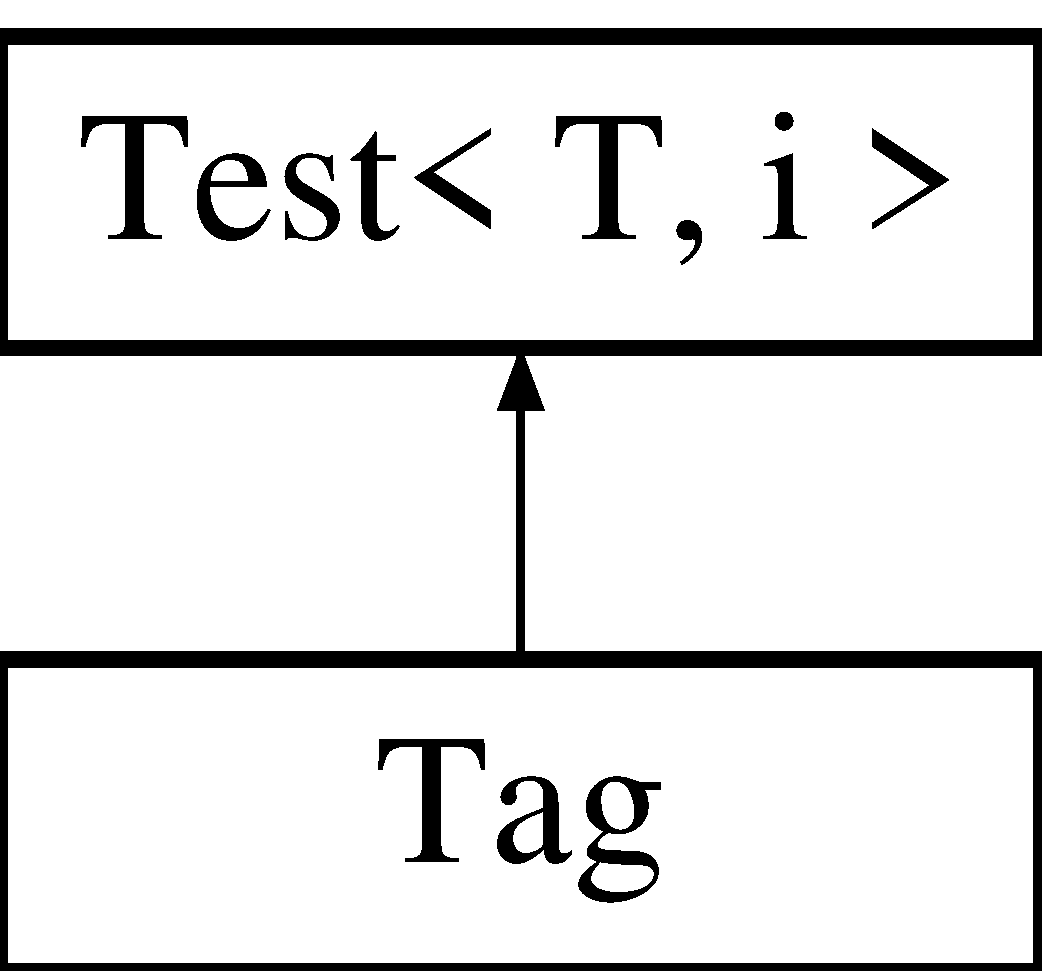
\includegraphics[height=2.000000cm]{class_tag}
\end{center}
\end{figure}
\subsection*{Public Member Functions}
\begin{DoxyCompactItemize}
\item 
void \hyperlink{class_tag_acc641ffae34e2c4c03a6edf0a513be28}{example} ()
\end{DoxyCompactItemize}
\subsection*{Additional Inherited Members}


\subsection{Detailed Description}
\hyperlink{class_a}{A} class that is inherited from the external class \hyperlink{class_test}{Test}. 

\subsection{Member Function Documentation}
\hypertarget{class_tag_acc641ffae34e2c4c03a6edf0a513be28}{\index{Tag@{Tag}!example@{example}}
\index{example@{example}!Tag@{Tag}}
\subsubsection[{example}]{\setlength{\rightskip}{0pt plus 5cm}void Tag\-::example (
\begin{DoxyParamCaption}
{}
\end{DoxyParamCaption}
)}}\label{class_tag_acc641ffae34e2c4c03a6edf0a513be28}
an overloaded member. 

The documentation for this class was generated from the following file\-:\begin{DoxyCompactItemize}
\item 
tag.\-cpp\end{DoxyCompactItemize}

\hypertarget{class_test}{\section{Test$<$ T, i $>$ Class Template Reference}
\label{class_test}\index{Test$<$ T, i $>$@{Test$<$ T, i $>$}}
}


This is a test class.  




{\ttfamily \#include \char`\"{}inc/class.\-h\char`\"{}}

Inheritance diagram for Test$<$ T, i $>$\-:\begin{figure}[H]
\begin{center}
\leavevmode
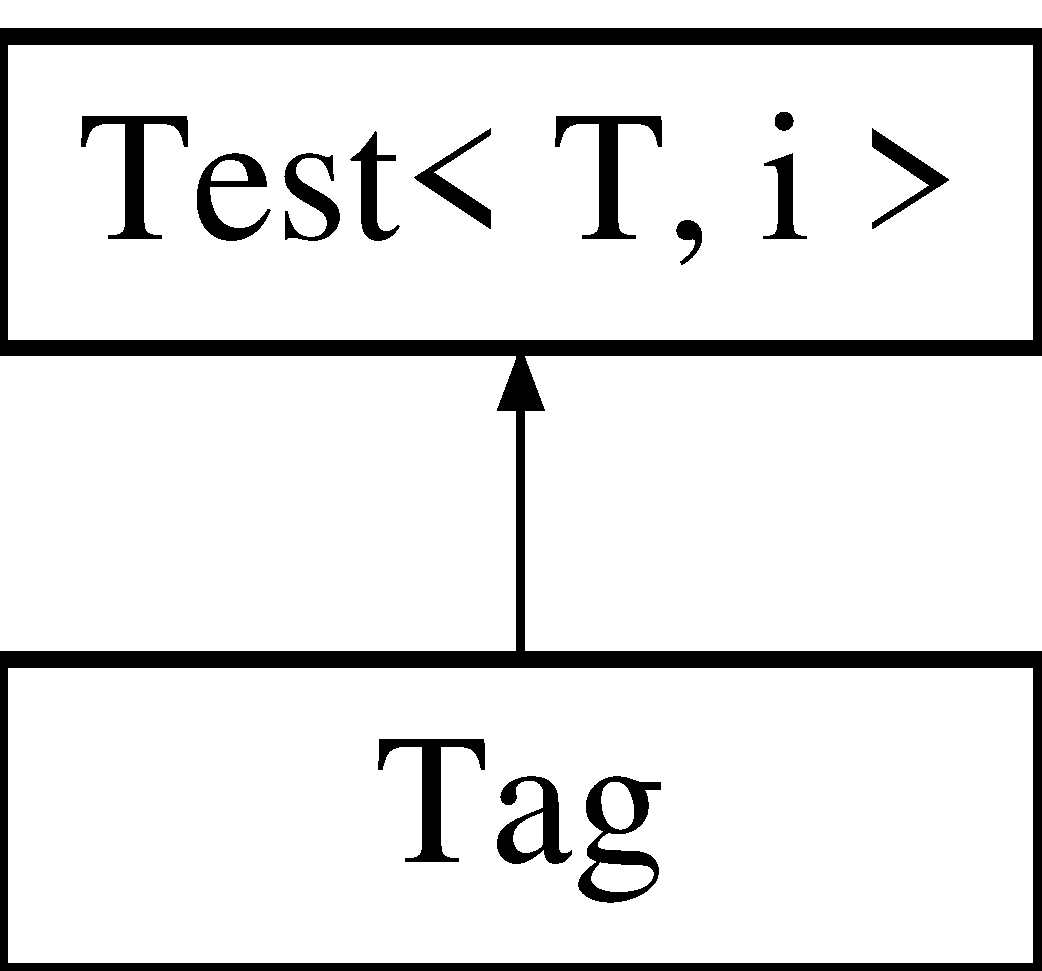
\includegraphics[height=2.000000cm]{class_test}
\end{center}
\end{figure}
\subsection*{Public Types}
\begin{DoxyCompactItemize}
\item 
enum \hyperlink{class_test_a26bf93efdaea3c6e2cfa4119c3755d3f}{Enum\-Type} \{ \hyperlink{class_test_a26bf93efdaea3c6e2cfa4119c3755d3fac5f5895ba2af9a9fa16f6840a45d659c}{E\-Val1}, 
\hyperlink{class_test_a26bf93efdaea3c6e2cfa4119c3755d3fa565724e73b1352aaa0af531d8018167e}{E\-Val2}
 \}
\item 
enum \hyperlink{class_test_a0653c5125502203305b6fe839e99ed01}{E\-Type} \{ \hyperlink{class_test_ad8d13fe56b896633273087859b89a1a3af621232782128e49458adf9069e126d4}{Val1}, 
\hyperlink{class_test_ad8d13fe56b896633273087859b89a1a3a218603a97012ef8dce0b798d598b2866}{Val2}
 \}
\item 
enum \hyperlink{class_test_ad8d13fe56b896633273087859b89a1a3}{T\-Enum} \{ \\*
\hyperlink{class_test_ad8d13fe56b896633273087859b89a1a3af621232782128e49458adf9069e126d4}{Val1}, 
\hyperlink{class_test_ad8d13fe56b896633273087859b89a1a3a218603a97012ef8dce0b798d598b2866}{Val2}, 
\hyperlink{class_test_ad8d13fe56b896633273087859b89a1a3a6db45e8c0b1d4e96e688fd43d343907a}{T\-Val1}, 
\hyperlink{class_test_ad8d13fe56b896633273087859b89a1a3a13b0433f996716c25158cecf9ee545c4}{T\-Val2}, 
\\*
\hyperlink{class_test_ad8d13fe56b896633273087859b89a1a3a5642b0033d6d17c4c9bee72133059f26}{T\-Val3}, 
\hyperlink{class_test_ad8d13fe56b896633273087859b89a1a3a6db45e8c0b1d4e96e688fd43d343907a}{T\-Val1}, 
\hyperlink{class_test_ad8d13fe56b896633273087859b89a1a3a13b0433f996716c25158cecf9ee545c4}{T\-Val2}, 
\hyperlink{class_test_ad8d13fe56b896633273087859b89a1a3a5642b0033d6d17c4c9bee72133059f26}{T\-Val3}
 \}
\item 
enum \hyperlink{class_test_a34b5b35cdcd492c108e62275d647bcf4}{Another\-Enum} \{ \hyperlink{class_test_a34b5b35cdcd492c108e62275d647bcf4a5e2c48aa2737365d177cfd29c88341f7}{V1}, 
\hyperlink{class_test_a34b5b35cdcd492c108e62275d647bcf4adb6734947779033dd3662483baa57be8}{V2}
 \}
\item 
enum \hyperlink{class_test_ad8d13fe56b896633273087859b89a1a3}{T\-Enum} \{ \\*
\hyperlink{class_test_ad8d13fe56b896633273087859b89a1a3af621232782128e49458adf9069e126d4}{Val1}, 
\hyperlink{class_test_ad8d13fe56b896633273087859b89a1a3a218603a97012ef8dce0b798d598b2866}{Val2}, 
\hyperlink{class_test_ad8d13fe56b896633273087859b89a1a3a6db45e8c0b1d4e96e688fd43d343907a}{T\-Val1}, 
\hyperlink{class_test_ad8d13fe56b896633273087859b89a1a3a13b0433f996716c25158cecf9ee545c4}{T\-Val2}, 
\\*
\hyperlink{class_test_ad8d13fe56b896633273087859b89a1a3a5642b0033d6d17c4c9bee72133059f26}{T\-Val3}, 
\hyperlink{class_test_ad8d13fe56b896633273087859b89a1a3a6db45e8c0b1d4e96e688fd43d343907a}{T\-Val1}, 
\hyperlink{class_test_ad8d13fe56b896633273087859b89a1a3a13b0433f996716c25158cecf9ee545c4}{T\-Val2}, 
\hyperlink{class_test_ad8d13fe56b896633273087859b89a1a3a5642b0033d6d17c4c9bee72133059f26}{T\-Val3}
 \}
\item 
enum \hyperlink{class_test_ad8d13fe56b896633273087859b89a1a3}{T\-Enum} \{ \\*
\hyperlink{class_test_ad8d13fe56b896633273087859b89a1a3af621232782128e49458adf9069e126d4}{Val1}, 
\hyperlink{class_test_ad8d13fe56b896633273087859b89a1a3a218603a97012ef8dce0b798d598b2866}{Val2}, 
\hyperlink{class_test_ad8d13fe56b896633273087859b89a1a3a6db45e8c0b1d4e96e688fd43d343907a}{T\-Val1}, 
\hyperlink{class_test_ad8d13fe56b896633273087859b89a1a3a13b0433f996716c25158cecf9ee545c4}{T\-Val2}, 
\\*
\hyperlink{class_test_ad8d13fe56b896633273087859b89a1a3a5642b0033d6d17c4c9bee72133059f26}{T\-Val3}, 
\hyperlink{class_test_ad8d13fe56b896633273087859b89a1a3a6db45e8c0b1d4e96e688fd43d343907a}{T\-Val1}, 
\hyperlink{class_test_ad8d13fe56b896633273087859b89a1a3a13b0433f996716c25158cecf9ee545c4}{T\-Val2}, 
\hyperlink{class_test_ad8d13fe56b896633273087859b89a1a3a5642b0033d6d17c4c9bee72133059f26}{T\-Val3}
 \}
\begin{DoxyCompactList}\small\item\em An enum. \end{DoxyCompactList}\end{DoxyCompactItemize}
\subsection*{Public Member Functions}
\begin{DoxyCompactItemize}
\item 
\hypertarget{class_test_a703997077e40c222687a0ea2973a9ea1}{void \hyperlink{class_test_a703997077e40c222687a0ea2973a9ea1}{member} ()}\label{class_test_a703997077e40c222687a0ea2973a9ea1}

\begin{DoxyCompactList}\small\item\em a member function. \end{DoxyCompactList}\item 
\hyperlink{class_test_a44e3a28c552193de099601e2910531f1}{Test} ()
\begin{DoxyCompactList}\small\item\em constructor \end{DoxyCompactList}\item 
\hyperlink{class_test_a31b169208ad4fc5344a7b6b8e1fd00c1}{$\sim$\-Test} ()
\begin{DoxyCompactList}\small\item\em destructor \end{DoxyCompactList}\item 
void \hyperlink{class_test_ac2f90eeb597ab8382dcdfcdf1df720f1}{member} (int)
\item 
void \hyperlink{class_test_aea163a1016f022bdb9e4acc3a32fa3eb}{member} (int, int)
\item 
void \hyperlink{class_test_a219565a812ad07b6517d74bdb36711ea}{example} ()
\item 
const char $\ast$ \hyperlink{class_test_a8a2453fcd30504975daa648a70a4e99e}{member} (char, int)  throw (std\-::out\-\_\-of\-\_\-range)
\begin{DoxyCompactList}\small\item\em \hyperlink{class_a}{A} member function. \end{DoxyCompactList}\item 
\hypertarget{class_test_a219565a812ad07b6517d74bdb36711ea}{void \hyperlink{class_test_a219565a812ad07b6517d74bdb36711ea}{example} ()}\label{class_test_a219565a812ad07b6517d74bdb36711ea}

\begin{DoxyCompactList}\small\item\em a member function \end{DoxyCompactList}\item 
\hyperlink{class_test_a44e3a28c552193de099601e2910531f1}{Test} ()
\item 
\hyperlink{class_test_a31b169208ad4fc5344a7b6b8e1fd00c1}{$\sim$\-Test} ()
\item 
int \hyperlink{class_test_ab89e4a0d841b51185817c5c7ae739ea4}{test\-Me} (int a, const char $\ast$s)
\item 
virtual void \hyperlink{class_test_ada2b629a324d987f40de6e72196526a5}{test\-Me\-Too} (char c1, char c2)=0
\item 
void \hyperlink{class_test_ae3d5d66760866dc4caf371ccef859ba6}{ungrouped\-Function} ()
\item 
void \hyperlink{class_test_a6b16f6be500388342845646c1969d3aa}{draw\-Rect} (int, int, int, int)
\item 
void \hyperlink{class_test_aadf47113ad9dcd5600cb22e3bcff5258}{draw\-Rect} (const Rect \&r)
\item 
\hyperlink{class_test_a44e3a28c552193de099601e2910531f1}{Test} ()
\begin{DoxyCompactList}\small\item\em \hyperlink{class_a}{A} constructor. \end{DoxyCompactList}\item 
\hyperlink{class_test_a31b169208ad4fc5344a7b6b8e1fd00c1}{$\sim$\-Test} ()
\begin{DoxyCompactList}\small\item\em \hyperlink{class_a}{A} destructor. \end{DoxyCompactList}\item 
int \hyperlink{class_test_ab89e4a0d841b51185817c5c7ae739ea4}{test\-Me} (int a, const char $\ast$s)
\begin{DoxyCompactList}\small\item\em \hyperlink{class_a}{A} normal member taking two arguments and returning an integer value. \end{DoxyCompactList}\item 
virtual void \hyperlink{class_test_ada2b629a324d987f40de6e72196526a5}{test\-Me\-Too} (char c1, char c2)=0
\begin{DoxyCompactList}\small\item\em \hyperlink{class_a}{A} pure virtual member. \end{DoxyCompactList}\item 
\hyperlink{class_test_adcf1bc755df94c4d07519c0a02aa1cc0}{Test} (const \hyperlink{class_test}{Test} \&)
\end{DoxyCompactItemize}
{\bf }\par
\begin{DoxyCompactItemize}
\item 
void \hyperlink{class_test_a63260e6eb6efa149aecf14f86c840c0b}{func1\-In\-Group1} ()
\item 
\hypertarget{class_test_a489fece588ea476e504db5177a157060}{void {\bfseries func2\-In\-Group1} ()}\label{class_test_a489fece588ea476e504db5177a157060}

\end{DoxyCompactItemize}

\subsection*{Public Attributes}
\begin{DoxyCompactItemize}
\item 
enum \hyperlink{class_test_ad8d13fe56b896633273087859b89a1a3}{Test\-::\-T\-Enum} $\ast$ \hyperlink{class_test_a8ee00d5158f7778385133989b5527742}{enum\-Ptr}
\begin{DoxyCompactList}\small\item\em Enum pointer. \end{DoxyCompactList}\item 
enum \hyperlink{class_test_ad8d13fe56b896633273087859b89a1a3}{Test\-::\-T\-Enum} \hyperlink{class_test_a13429658c8d90928b16ec109e32f88b5}{enum\-Var}
\begin{DoxyCompactList}\small\item\em Enum variable. \end{DoxyCompactList}\item 
int \hyperlink{class_test_aba22fd8dcb6ca747e2266fadaf5bc383}{public\-Var}
\begin{DoxyCompactList}\small\item\em \hyperlink{class_a}{A} public variable. \end{DoxyCompactList}\item 
int($\ast$ \hyperlink{class_test_a2ce50e60d16f5071772c6acde08181bd}{handler} )(int a, int b)
\begin{DoxyCompactList}\small\item\em \hyperlink{class_a}{A} function variable. \end{DoxyCompactList}\end{DoxyCompactItemize}
\subsection*{Protected Attributes}
\begin{DoxyCompactItemize}
\item 
int \hyperlink{class_test_aefcbb7ead19f2c28a71a3a3f26cef6cb}{value}
\item 
int \hyperlink{class_test_ae75d55c8cf6390227d51c0965a4de296}{var}
\end{DoxyCompactItemize}
\subsection*{Group2}
\label{_amgrp6be2faefeff8740e94471f5ae04da6d0}%
Description of group 2. \begin{DoxyCompactItemize}
\item 
void \hyperlink{class_test_a627da802edbda6cebe0849202e3da85e}{func1\-In\-Group2} ()
\item 
void \hyperlink{class_test_ae6d5e6f9e0d9ac70e976be7476499b74}{func2\-In\-Group2} ()
\end{DoxyCompactItemize}


\subsection{Detailed Description}
\subsubsection*{template$<$class T, int i = 100$>$class Test$<$ T, i $>$}

This is a test class. 

\hyperlink{class_a}{A} short description.

\hyperlink{class_test}{Test} class.

\hyperlink{class_a}{A} test class

Since this documentation block belongs to the class \hyperlink{class_test}{Test} no link to \hyperlink{class_test}{Test} is generated.

Two ways to link to a constructor are\-: \hyperlink{class_test}{Test} and \hyperlink{class_test_a44e3a28c552193de099601e2910531f1}{Test()}.

Links to the destructor are\-: \hyperlink{class_test_a31b169208ad4fc5344a7b6b8e1fd00c1}{$\sim$\-Test} and \hyperlink{class_test_a31b169208ad4fc5344a7b6b8e1fd00c1}{$\sim$\-Test()}.

\hyperlink{class_a}{A} link to a member in this class\-: \hyperlink{class_test_a703997077e40c222687a0ea2973a9ea1}{member()}.

More specific links to the each of the overloaded members\-: \hyperlink{class_test_ac2f90eeb597ab8382dcdfcdf1df720f1}{member(int)} and \hyperlink{class_test_aea163a1016f022bdb9e4acc3a32fa3eb}{member(int,int)}.

\hyperlink{class_a}{A} link to the variable \hyperlink{class_test_ae75d55c8cf6390227d51c0965a4de296}{var}.

\hyperlink{class_a}{A} link to the global typedef \hyperlink{class_b}{B}.

\hyperlink{class_a}{A} link to the global enumeration type \hyperlink{autolink_8cpp_a656d63cf384d2a6f23c2c18523a7bc5e}{Glob\-Enum}.

\hyperlink{class_a}{A} link to the define \hyperlink{define_8h_a996f7be338ccb40d1a2a5abc1ad61759}{A\-B\-S(x)}.

\hyperlink{class_a}{A} link to a variable \hyperlink{class_test_ae75d55c8cf6390227d51c0965a4de296}{using another text} as a link.

\hyperlink{class_a}{A} link to the enumeration type \hyperlink{class_test_a0653c5125502203305b6fe839e99ed01}{E\-Type}.

\hyperlink{class_a}{A} link to some enumeration values\-: \hyperlink{class_test_ad8d13fe56b896633273087859b89a1a3af621232782128e49458adf9069e126d4}{Val1 } and \hyperlink{autolink_8cpp_a656d63cf384d2a6f23c2c18523a7bc5ea0f016f49e4f3bcd072319b9d68bc927d}{G\-Val1}.

And last but not least a link to a file\-: \hyperlink{autolink_8cpp}{autolink.\-cpp}.

\begin{DoxySeeAlso}{See Also}
Inside a see also section any word is checked, so \hyperlink{class_test_a0653c5125502203305b6fe839e99ed01}{E\-Type}, \hyperlink{class_test_ad8d13fe56b896633273087859b89a1a3af621232782128e49458adf9069e126d4}{Val1}, \hyperlink{autolink_8cpp_a656d63cf384d2a6f23c2c18523a7bc5ea0f016f49e4f3bcd072319b9d68bc927d}{G\-Val1}, \hyperlink{class_test_a31b169208ad4fc5344a7b6b8e1fd00c1}{$\sim$\-Test} and \hyperlink{class_test_a703997077e40c222687a0ea2973a9ea1}{member} will be replaced by links in H\-T\-M\-L.
\end{DoxySeeAlso}
\hyperlink{class_a}{A} \hyperlink{class_test}{Test} class. More details about this class.

\hyperlink{class_a}{A} test class.

\hyperlink{class_a}{A} test class. \hyperlink{class_a}{A} more elaborate class description.

\hyperlink{class_a}{A} class. Details

\hyperlink{class_a}{A} more elaborate class description.

\hyperlink{class_a}{A} template class

Some details about the \hyperlink{class_test}{Test} class

The class description.

Details about \hyperlink{class_test}{Test}.

More text.

Normal text.

\begin{DoxyParagraph}{User defined paragraph\-:}
Contents of the paragraph.
\end{DoxyParagraph}
\begin{DoxyParagraph}{}
New paragraph under the same heading.
\end{DoxyParagraph}
\begin{DoxyNote}{Note}
This note consists of two paragraphs. This is the first paragraph.
\end{DoxyNote}
\begin{DoxyParagraph}{}
And this is the second paragraph.
\end{DoxyParagraph}
More normal text. 

\subsection{Member Enumeration Documentation}
\hypertarget{class_test_a34b5b35cdcd492c108e62275d647bcf4}{\index{Test@{Test}!Another\-Enum@{Another\-Enum}}
\index{Another\-Enum@{Another\-Enum}!Test@{Test}}
\subsubsection[{Another\-Enum}]{\setlength{\rightskip}{0pt plus 5cm}template$<$class T , int i = 100$>$ enum {\bf Test\-::\-Another\-Enum}}}\label{class_test_a34b5b35cdcd492c108e62275d647bcf4}
Another enum, with inline docs \begin{Desc}
\item[Enumerator\-: ]\par
\begin{description}
\index{V1@{V1}!Test@{Test}}\index{Test@{Test}!V1@{V1}}\item[{\em 
\hypertarget{class_test_a34b5b35cdcd492c108e62275d647bcf4a5e2c48aa2737365d177cfd29c88341f7}{V1}\label{class_test_a34b5b35cdcd492c108e62275d647bcf4a5e2c48aa2737365d177cfd29c88341f7}
}]value 1 \index{V2@{V2}!Test@{Test}}\index{Test@{Test}!V2@{V2}}\item[{\em 
\hypertarget{class_test_a34b5b35cdcd492c108e62275d647bcf4adb6734947779033dd3662483baa57be8}{V2}\label{class_test_a34b5b35cdcd492c108e62275d647bcf4adb6734947779033dd3662483baa57be8}
}]value 2 \end{description}
\end{Desc}

\hypertarget{class_test_a26bf93efdaea3c6e2cfa4119c3755d3f}{\index{Test@{Test}!Enum\-Type@{Enum\-Type}}
\index{Enum\-Type@{Enum\-Type}!Test@{Test}}
\subsubsection[{Enum\-Type}]{\setlength{\rightskip}{0pt plus 5cm}template$<$class T , int i = 100$>$ enum {\bf Test\-::\-Enum\-Type}}}\label{class_test_a26bf93efdaea3c6e2cfa4119c3755d3f}
An enum type. The documentation block cannot be put after the enum! \begin{Desc}
\item[Enumerator\-: ]\par
\begin{description}
\index{E\-Val1@{E\-Val1}!Test@{Test}}\index{Test@{Test}!E\-Val1@{E\-Val1}}\item[{\em 
\hypertarget{class_test_a26bf93efdaea3c6e2cfa4119c3755d3fac5f5895ba2af9a9fa16f6840a45d659c}{E\-Val1}\label{class_test_a26bf93efdaea3c6e2cfa4119c3755d3fac5f5895ba2af9a9fa16f6840a45d659c}
}]enum value 1 \index{E\-Val2@{E\-Val2}!Test@{Test}}\index{Test@{Test}!E\-Val2@{E\-Val2}}\item[{\em 
\hypertarget{class_test_a26bf93efdaea3c6e2cfa4119c3755d3fa565724e73b1352aaa0af531d8018167e}{E\-Val2}\label{class_test_a26bf93efdaea3c6e2cfa4119c3755d3fa565724e73b1352aaa0af531d8018167e}
}]enum value 2 \end{description}
\end{Desc}

\hypertarget{class_test_a0653c5125502203305b6fe839e99ed01}{\index{Test@{Test}!E\-Type@{E\-Type}}
\index{E\-Type@{E\-Type}!Test@{Test}}
\subsubsection[{E\-Type}]{\setlength{\rightskip}{0pt plus 5cm}template$<$class T , int i = 100$>$ enum {\bf Test\-::\-E\-Type}}}\label{class_test_a0653c5125502203305b6fe839e99ed01}
An enum type. More details \begin{Desc}
\item[Enumerator\-: ]\par
\begin{description}
\index{Val1@{Val1}!Test@{Test}}\index{Test@{Test}!Val1@{Val1}}\item[{\em 
\hypertarget{class_test_ad8d13fe56b896633273087859b89a1a3af621232782128e49458adf9069e126d4}{Val1}\label{class_test_ad8d13fe56b896633273087859b89a1a3af621232782128e49458adf9069e126d4}
}]enum value 1

The description of the first enum value. \index{Val2@{Val2}!Test@{Test}}\index{Test@{Test}!Val2@{Val2}}\item[{\em 
\hypertarget{class_test_ad8d13fe56b896633273087859b89a1a3a218603a97012ef8dce0b798d598b2866}{Val2}\label{class_test_ad8d13fe56b896633273087859b89a1a3a218603a97012ef8dce0b798d598b2866}
}]enum value 2 \end{description}
\end{Desc}

\hypertarget{class_test_ad8d13fe56b896633273087859b89a1a3}{\index{Test@{Test}!T\-Enum@{T\-Enum}}
\index{T\-Enum@{T\-Enum}!Test@{Test}}
\subsubsection[{T\-Enum}]{\setlength{\rightskip}{0pt plus 5cm}template$<$class T , int i = 100$>$ enum {\bf Test\-::\-T\-Enum}}}\label{class_test_ad8d13fe56b896633273087859b89a1a3}
\hyperlink{class_a}{A} description of the enum type. \begin{Desc}
\item[Enumerator\-: ]\par
\begin{description}
\index{Val1@{Val1}!Test@{Test}}\index{Test@{Test}!Val1@{Val1}}\item[{\em 
\hypertarget{class_test_ad8d13fe56b896633273087859b89a1a3af621232782128e49458adf9069e126d4}{Val1}\label{class_test_ad8d13fe56b896633273087859b89a1a3af621232782128e49458adf9069e126d4}
}]enum value 1

The description of the first enum value. \index{Val2@{Val2}!Test@{Test}}\index{Test@{Test}!Val2@{Val2}}\item[{\em 
\hypertarget{class_test_ad8d13fe56b896633273087859b89a1a3a218603a97012ef8dce0b798d598b2866}{Val2}\label{class_test_ad8d13fe56b896633273087859b89a1a3a218603a97012ef8dce0b798d598b2866}
}]enum value 2 \index{T\-Val1@{T\-Val1}!Test@{Test}}\index{Test@{Test}!T\-Val1@{T\-Val1}}\item[{\em 
\hypertarget{class_test_ad8d13fe56b896633273087859b89a1a3a6db45e8c0b1d4e96e688fd43d343907a}{T\-Val1}\label{class_test_ad8d13fe56b896633273087859b89a1a3a6db45e8c0b1d4e96e688fd43d343907a}
}]enum value T\-Val1.

Enum value T\-Val1. \index{T\-Val2@{T\-Val2}!Test@{Test}}\index{Test@{Test}!T\-Val2@{T\-Val2}}\item[{\em 
\hypertarget{class_test_ad8d13fe56b896633273087859b89a1a3a13b0433f996716c25158cecf9ee545c4}{T\-Val2}\label{class_test_ad8d13fe56b896633273087859b89a1a3a13b0433f996716c25158cecf9ee545c4}
}]enum value T\-Val2.

Enum value T\-Val2. \index{T\-Val3@{T\-Val3}!Test@{Test}}\index{Test@{Test}!T\-Val3@{T\-Val3}}\item[{\em 
\hypertarget{class_test_ad8d13fe56b896633273087859b89a1a3a5642b0033d6d17c4c9bee72133059f26}{T\-Val3}\label{class_test_ad8d13fe56b896633273087859b89a1a3a5642b0033d6d17c4c9bee72133059f26}
}]enum value T\-Val3.

Enum value T\-Val3. \index{T\-Val1@{T\-Val1}!Test@{Test}}\index{Test@{Test}!T\-Val1@{T\-Val1}}\item[{\em 
\hypertarget{class_test_ad8d13fe56b896633273087859b89a1a3a6db45e8c0b1d4e96e688fd43d343907a}{T\-Val1}\label{class_test_ad8d13fe56b896633273087859b89a1a3a6db45e8c0b1d4e96e688fd43d343907a}
}]enum value T\-Val1.

Enum value T\-Val1. \index{T\-Val2@{T\-Val2}!Test@{Test}}\index{Test@{Test}!T\-Val2@{T\-Val2}}\item[{\em 
\hypertarget{class_test_ad8d13fe56b896633273087859b89a1a3a13b0433f996716c25158cecf9ee545c4}{T\-Val2}\label{class_test_ad8d13fe56b896633273087859b89a1a3a13b0433f996716c25158cecf9ee545c4}
}]enum value T\-Val2.

Enum value T\-Val2. \index{T\-Val3@{T\-Val3}!Test@{Test}}\index{Test@{Test}!T\-Val3@{T\-Val3}}\item[{\em 
\hypertarget{class_test_ad8d13fe56b896633273087859b89a1a3a5642b0033d6d17c4c9bee72133059f26}{T\-Val3}\label{class_test_ad8d13fe56b896633273087859b89a1a3a5642b0033d6d17c4c9bee72133059f26}
}]enum value T\-Val3.

Enum value T\-Val3. \end{description}
\end{Desc}

\hypertarget{class_test_ad8d13fe56b896633273087859b89a1a3}{\index{Test@{Test}!T\-Enum@{T\-Enum}}
\index{T\-Enum@{T\-Enum}!Test@{Test}}
\subsubsection[{T\-Enum}]{\setlength{\rightskip}{0pt plus 5cm}template$<$class T , int i = 100$>$ enum {\bf Test\-::\-T\-Enum}}}\label{class_test_ad8d13fe56b896633273087859b89a1a3}


An enum. 

More detailed enum description. \begin{Desc}
\item[Enumerator\-: ]\par
\begin{description}
\index{Val1@{Val1}!Test@{Test}}\index{Test@{Test}!Val1@{Val1}}\item[{\em 
\hypertarget{class_test_ad8d13fe56b896633273087859b89a1a3af621232782128e49458adf9069e126d4}{Val1}\label{class_test_ad8d13fe56b896633273087859b89a1a3af621232782128e49458adf9069e126d4}
}]enum value 1

The description of the first enum value. \index{Val2@{Val2}!Test@{Test}}\index{Test@{Test}!Val2@{Val2}}\item[{\em 
\hypertarget{class_test_ad8d13fe56b896633273087859b89a1a3a218603a97012ef8dce0b798d598b2866}{Val2}\label{class_test_ad8d13fe56b896633273087859b89a1a3a218603a97012ef8dce0b798d598b2866}
}]enum value 2 \index{T\-Val1@{T\-Val1}!Test@{Test}}\index{Test@{Test}!T\-Val1@{T\-Val1}}\item[{\em 
\hypertarget{class_test_ad8d13fe56b896633273087859b89a1a3a6db45e8c0b1d4e96e688fd43d343907a}{T\-Val1}\label{class_test_ad8d13fe56b896633273087859b89a1a3a6db45e8c0b1d4e96e688fd43d343907a}
}]enum value T\-Val1.

Enum value T\-Val1. \index{T\-Val2@{T\-Val2}!Test@{Test}}\index{Test@{Test}!T\-Val2@{T\-Val2}}\item[{\em 
\hypertarget{class_test_ad8d13fe56b896633273087859b89a1a3a13b0433f996716c25158cecf9ee545c4}{T\-Val2}\label{class_test_ad8d13fe56b896633273087859b89a1a3a13b0433f996716c25158cecf9ee545c4}
}]enum value T\-Val2.

Enum value T\-Val2. \index{T\-Val3@{T\-Val3}!Test@{Test}}\index{Test@{Test}!T\-Val3@{T\-Val3}}\item[{\em 
\hypertarget{class_test_ad8d13fe56b896633273087859b89a1a3a5642b0033d6d17c4c9bee72133059f26}{T\-Val3}\label{class_test_ad8d13fe56b896633273087859b89a1a3a5642b0033d6d17c4c9bee72133059f26}
}]enum value T\-Val3.

Enum value T\-Val3. \index{T\-Val1@{T\-Val1}!Test@{Test}}\index{Test@{Test}!T\-Val1@{T\-Val1}}\item[{\em 
\hypertarget{class_test_ad8d13fe56b896633273087859b89a1a3a6db45e8c0b1d4e96e688fd43d343907a}{T\-Val1}\label{class_test_ad8d13fe56b896633273087859b89a1a3a6db45e8c0b1d4e96e688fd43d343907a}
}]enum value T\-Val1.

Enum value T\-Val1. \index{T\-Val2@{T\-Val2}!Test@{Test}}\index{Test@{Test}!T\-Val2@{T\-Val2}}\item[{\em 
\hypertarget{class_test_ad8d13fe56b896633273087859b89a1a3a13b0433f996716c25158cecf9ee545c4}{T\-Val2}\label{class_test_ad8d13fe56b896633273087859b89a1a3a13b0433f996716c25158cecf9ee545c4}
}]enum value T\-Val2.

Enum value T\-Val2. \index{T\-Val3@{T\-Val3}!Test@{Test}}\index{Test@{Test}!T\-Val3@{T\-Val3}}\item[{\em 
\hypertarget{class_test_ad8d13fe56b896633273087859b89a1a3a5642b0033d6d17c4c9bee72133059f26}{T\-Val3}\label{class_test_ad8d13fe56b896633273087859b89a1a3a5642b0033d6d17c4c9bee72133059f26}
}]enum value T\-Val3.

Enum value T\-Val3. \end{description}
\end{Desc}

\hypertarget{class_test_ad8d13fe56b896633273087859b89a1a3}{\index{Test@{Test}!T\-Enum@{T\-Enum}}
\index{T\-Enum@{T\-Enum}!Test@{Test}}
\subsubsection[{T\-Enum}]{\setlength{\rightskip}{0pt plus 5cm}template$<$class T , int i = 100$>$ enum {\bf Test\-::\-T\-Enum}}}\label{class_test_ad8d13fe56b896633273087859b89a1a3}
An enum. More detailed enum description. \begin{Desc}
\item[Enumerator\-: ]\par
\begin{description}
\index{Val1@{Val1}!Test@{Test}}\index{Test@{Test}!Val1@{Val1}}\item[{\em 
\hypertarget{class_test_ad8d13fe56b896633273087859b89a1a3af621232782128e49458adf9069e126d4}{Val1}\label{class_test_ad8d13fe56b896633273087859b89a1a3af621232782128e49458adf9069e126d4}
}]enum value 1

The description of the first enum value. \index{Val2@{Val2}!Test@{Test}}\index{Test@{Test}!Val2@{Val2}}\item[{\em 
\hypertarget{class_test_ad8d13fe56b896633273087859b89a1a3a218603a97012ef8dce0b798d598b2866}{Val2}\label{class_test_ad8d13fe56b896633273087859b89a1a3a218603a97012ef8dce0b798d598b2866}
}]enum value 2 \index{T\-Val1@{T\-Val1}!Test@{Test}}\index{Test@{Test}!T\-Val1@{T\-Val1}}\item[{\em 
\hypertarget{class_test_ad8d13fe56b896633273087859b89a1a3a6db45e8c0b1d4e96e688fd43d343907a}{T\-Val1}\label{class_test_ad8d13fe56b896633273087859b89a1a3a6db45e8c0b1d4e96e688fd43d343907a}
}]enum value T\-Val1.

Enum value T\-Val1. \index{T\-Val2@{T\-Val2}!Test@{Test}}\index{Test@{Test}!T\-Val2@{T\-Val2}}\item[{\em 
\hypertarget{class_test_ad8d13fe56b896633273087859b89a1a3a13b0433f996716c25158cecf9ee545c4}{T\-Val2}\label{class_test_ad8d13fe56b896633273087859b89a1a3a13b0433f996716c25158cecf9ee545c4}
}]enum value T\-Val2.

Enum value T\-Val2. \index{T\-Val3@{T\-Val3}!Test@{Test}}\index{Test@{Test}!T\-Val3@{T\-Val3}}\item[{\em 
\hypertarget{class_test_ad8d13fe56b896633273087859b89a1a3a5642b0033d6d17c4c9bee72133059f26}{T\-Val3}\label{class_test_ad8d13fe56b896633273087859b89a1a3a5642b0033d6d17c4c9bee72133059f26}
}]enum value T\-Val3.

Enum value T\-Val3. \index{T\-Val1@{T\-Val1}!Test@{Test}}\index{Test@{Test}!T\-Val1@{T\-Val1}}\item[{\em 
\hypertarget{class_test_ad8d13fe56b896633273087859b89a1a3a6db45e8c0b1d4e96e688fd43d343907a}{T\-Val1}\label{class_test_ad8d13fe56b896633273087859b89a1a3a6db45e8c0b1d4e96e688fd43d343907a}
}]enum value T\-Val1.

Enum value T\-Val1. \index{T\-Val2@{T\-Val2}!Test@{Test}}\index{Test@{Test}!T\-Val2@{T\-Val2}}\item[{\em 
\hypertarget{class_test_ad8d13fe56b896633273087859b89a1a3a13b0433f996716c25158cecf9ee545c4}{T\-Val2}\label{class_test_ad8d13fe56b896633273087859b89a1a3a13b0433f996716c25158cecf9ee545c4}
}]enum value T\-Val2.

Enum value T\-Val2. \index{T\-Val3@{T\-Val3}!Test@{Test}}\index{Test@{Test}!T\-Val3@{T\-Val3}}\item[{\em 
\hypertarget{class_test_ad8d13fe56b896633273087859b89a1a3a5642b0033d6d17c4c9bee72133059f26}{T\-Val3}\label{class_test_ad8d13fe56b896633273087859b89a1a3a5642b0033d6d17c4c9bee72133059f26}
}]enum value T\-Val3.

Enum value T\-Val3. \end{description}
\end{Desc}



\subsection{Constructor \& Destructor Documentation}
\hypertarget{class_test_a44e3a28c552193de099601e2910531f1}{\index{Test@{Test}!Test@{Test}}
\index{Test@{Test}!Test@{Test}}
\subsubsection[{Test}]{\setlength{\rightskip}{0pt plus 5cm}template$<$class T , int i$>$ {\bf Test}$<$ T, i $>$\-::{\bf Test} (
\begin{DoxyParamCaption}
{}
\end{DoxyParamCaption}
)}}\label{class_test_a44e3a28c552193de099601e2910531f1}


constructor 

details.

The constructor of the template class \hypertarget{class_test_a31b169208ad4fc5344a7b6b8e1fd00c1}{\index{Test@{Test}!$\sim$\-Test@{$\sim$\-Test}}
\index{$\sim$\-Test@{$\sim$\-Test}!Test@{Test}}
\subsubsection[{$\sim$\-Test}]{\setlength{\rightskip}{0pt plus 5cm}template$<$class T , int i = 100$>$ {\bf Test}$<$ T, i $>$\-::$\sim${\bf Test} (
\begin{DoxyParamCaption}
{}
\end{DoxyParamCaption}
)}}\label{class_test_a31b169208ad4fc5344a7b6b8e1fd00c1}


destructor 

details. \hypertarget{class_test_a44e3a28c552193de099601e2910531f1}{\index{Test@{Test}!Test@{Test}}
\index{Test@{Test}!Test@{Test}}
\subsubsection[{Test}]{\setlength{\rightskip}{0pt plus 5cm}template$<$class T , int i = 100$>$ {\bf Test}$<$ T, i $>$\-::{\bf Test} (
\begin{DoxyParamCaption}
{}
\end{DoxyParamCaption}
)}}\label{class_test_a44e3a28c552193de099601e2910531f1}
\hyperlink{class_a}{A} constructor. \hyperlink{class_a}{A} more elaborate description of the constructor. \hypertarget{class_test_a31b169208ad4fc5344a7b6b8e1fd00c1}{\index{Test@{Test}!$\sim$\-Test@{$\sim$\-Test}}
\index{$\sim$\-Test@{$\sim$\-Test}!Test@{Test}}
\subsubsection[{$\sim$\-Test}]{\setlength{\rightskip}{0pt plus 5cm}template$<$class T , int i = 100$>$ {\bf Test}$<$ T, i $>$\-::$\sim${\bf Test} (
\begin{DoxyParamCaption}
{}
\end{DoxyParamCaption}
)}}\label{class_test_a31b169208ad4fc5344a7b6b8e1fd00c1}
\hyperlink{class_a}{A} destructor. \hyperlink{class_a}{A} more elaborate description of the destructor. \hypertarget{class_test_a44e3a28c552193de099601e2910531f1}{\index{Test@{Test}!Test@{Test}}
\index{Test@{Test}!Test@{Test}}
\subsubsection[{Test}]{\setlength{\rightskip}{0pt plus 5cm}template$<$class T , int i = 100$>$ {\bf Test}$<$ T, i $>$\-::{\bf Test} (
\begin{DoxyParamCaption}
{}
\end{DoxyParamCaption}
)}}\label{class_test_a44e3a28c552193de099601e2910531f1}


\hyperlink{class_a}{A} constructor. 

\hyperlink{class_a}{A} more elaborate description of the constructor. \hypertarget{class_test_a31b169208ad4fc5344a7b6b8e1fd00c1}{\index{Test@{Test}!$\sim$\-Test@{$\sim$\-Test}}
\index{$\sim$\-Test@{$\sim$\-Test}!Test@{Test}}
\subsubsection[{$\sim$\-Test}]{\setlength{\rightskip}{0pt plus 5cm}template$<$class T , int i = 100$>$ {\bf Test}$<$ T, i $>$\-::$\sim${\bf Test} (
\begin{DoxyParamCaption}
{}
\end{DoxyParamCaption}
)}}\label{class_test_a31b169208ad4fc5344a7b6b8e1fd00c1}


\hyperlink{class_a}{A} destructor. 

\hyperlink{class_a}{A} more elaborate description of the destructor. \hypertarget{class_test_adcf1bc755df94c4d07519c0a02aa1cc0}{\index{Test@{Test}!Test@{Test}}
\index{Test@{Test}!Test@{Test}}
\subsubsection[{Test}]{\setlength{\rightskip}{0pt plus 5cm}template$<$class T , int i$>$ {\bf Test}$<$ T, i $>$\-::{\bf Test} (
\begin{DoxyParamCaption}
\item[{const {\bf Test}$<$ T, i $>$ \&}]{t}
\end{DoxyParamCaption}
)}}\label{class_test_adcf1bc755df94c4d07519c0a02aa1cc0}
The copy constructor 

\subsection{Member Function Documentation}
\hypertarget{class_test_a6b16f6be500388342845646c1969d3aa}{\index{Test@{Test}!draw\-Rect@{draw\-Rect}}
\index{draw\-Rect@{draw\-Rect}!Test@{Test}}
\subsubsection[{draw\-Rect}]{\setlength{\rightskip}{0pt plus 5cm}template$<$class T , int i = 100$>$ void {\bf Test}$<$ T, i $>$\-::draw\-Rect (
\begin{DoxyParamCaption}
\item[{int}]{x, }
\item[{int}]{y, }
\item[{int}]{w, }
\item[{int}]{h}
\end{DoxyParamCaption}
)}}\label{class_test_a6b16f6be500388342845646c1969d3aa}
This command draws a rectangle with a left upper corner at ( {\itshape x} , {\itshape y} ), width {\itshape w} and height {\itshape h}. \hypertarget{class_test_aadf47113ad9dcd5600cb22e3bcff5258}{\index{Test@{Test}!draw\-Rect@{draw\-Rect}}
\index{draw\-Rect@{draw\-Rect}!Test@{Test}}
\subsubsection[{draw\-Rect}]{\setlength{\rightskip}{0pt plus 5cm}template$<$class T , int i = 100$>$ void {\bf Test}$<$ T, i $>$\-::draw\-Rect (
\begin{DoxyParamCaption}
\item[{const Rect \&}]{r}
\end{DoxyParamCaption}
)}}\label{class_test_aadf47113ad9dcd5600cb22e3bcff5258}
This is an overloaded member function, provided for convenience. It differs from the above function only in what argument(s) it accepts. \hypertarget{class_test_a219565a812ad07b6517d74bdb36711ea}{\index{Test@{Test}!example@{example}}
\index{example@{example}!Test@{Test}}
\subsubsection[{example}]{\setlength{\rightskip}{0pt plus 5cm}template$<$class T , int i = 100$>$ void {\bf Test}$<$ T, i $>$\-::example (
\begin{DoxyParamCaption}
{}
\end{DoxyParamCaption}
)}}\label{class_test_a219565a812ad07b6517d74bdb36711ea}
An example member function. More details about this function. \hypertarget{class_test_a63260e6eb6efa149aecf14f86c840c0b}{\index{Test@{Test}!func1\-In\-Group1@{func1\-In\-Group1}}
\index{func1\-In\-Group1@{func1\-In\-Group1}!Test@{Test}}
\subsubsection[{func1\-In\-Group1}]{\setlength{\rightskip}{0pt plus 5cm}template$<$class T , int i = 100$>$ void {\bf Test}$<$ T, i $>$\-::func1\-In\-Group1 (
\begin{DoxyParamCaption}
{}
\end{DoxyParamCaption}
)}}\label{class_test_a63260e6eb6efa149aecf14f86c840c0b}
Same documentation for both members. Details \hypertarget{class_test_a627da802edbda6cebe0849202e3da85e}{\index{Test@{Test}!func1\-In\-Group2@{func1\-In\-Group2}}
\index{func1\-In\-Group2@{func1\-In\-Group2}!Test@{Test}}
\subsubsection[{func1\-In\-Group2}]{\setlength{\rightskip}{0pt plus 5cm}template$<$class T , int i = 100$>$ void {\bf Test}$<$ T, i $>$\-::func1\-In\-Group2 (
\begin{DoxyParamCaption}
{}
\end{DoxyParamCaption}
)}}\label{class_test_a627da802edbda6cebe0849202e3da85e}
Function 1 in group 2. Details. \hypertarget{class_test_ae6d5e6f9e0d9ac70e976be7476499b74}{\index{Test@{Test}!func2\-In\-Group2@{func2\-In\-Group2}}
\index{func2\-In\-Group2@{func2\-In\-Group2}!Test@{Test}}
\subsubsection[{func2\-In\-Group2}]{\setlength{\rightskip}{0pt plus 5cm}template$<$class T , int i = 100$>$ void {\bf Test}$<$ T, i $>$\-::func2\-In\-Group2 (
\begin{DoxyParamCaption}
{}
\end{DoxyParamCaption}
)\hspace{0.3cm}{\ttfamily [protected]}}}\label{class_test_ae6d5e6f9e0d9ac70e976be7476499b74}
Function 2 in group 2. Details. \hypertarget{class_test_a8a2453fcd30504975daa648a70a4e99e}{\index{Test@{Test}!member@{member}}
\index{member@{member}!Test@{Test}}
\subsubsection[{member}]{\setlength{\rightskip}{0pt plus 5cm}template$<$class T , int i = 100$>$ const char $\ast$ {\bf Test}$<$ T, i $>$\-::member (
\begin{DoxyParamCaption}
\item[{char}]{c, }
\item[{int}]{n}
\end{DoxyParamCaption}
)  throw (std\-::out\-\_\-of\-\_\-range)}}\label{class_test_a8a2453fcd30504975daa648a70a4e99e}


\hyperlink{class_a}{A} member function. 


\begin{DoxyParams}{Parameters}
{\em c} & a character. \\
\hline
{\em n} & an integer. \\
\hline
\end{DoxyParams}

\begin{DoxyExceptions}{Exceptions}
{\em std\-::out\-\_\-of\-\_\-range} & parameter is out of range. \\
\hline
\end{DoxyExceptions}
\begin{DoxyReturn}{Returns}
a character pointer. 
\end{DoxyReturn}
\hypertarget{class_test_ac2f90eeb597ab8382dcdfcdf1df720f1}{\index{Test@{Test}!member@{member}}
\index{member@{member}!Test@{Test}}
\subsubsection[{member}]{\setlength{\rightskip}{0pt plus 5cm}template$<$class T , int i = 100$>$ void {\bf Test}$<$ T, i $>$\-::member (
\begin{DoxyParamCaption}
\item[{int}]{}
\end{DoxyParamCaption}
)}}\label{class_test_ac2f90eeb597ab8382dcdfcdf1df720f1}
\hyperlink{class_a}{A} member function. Details. \hypertarget{class_test_aea163a1016f022bdb9e4acc3a32fa3eb}{\index{Test@{Test}!member@{member}}
\index{member@{member}!Test@{Test}}
\subsubsection[{member}]{\setlength{\rightskip}{0pt plus 5cm}template$<$class T , int i = 100$>$ void {\bf Test}$<$ T, i $>$\-::member (
\begin{DoxyParamCaption}
\item[{int}]{, }
\item[{int}]{}
\end{DoxyParamCaption}
)}}\label{class_test_aea163a1016f022bdb9e4acc3a32fa3eb}
An overloaded member function. Details \hypertarget{class_test_ab89e4a0d841b51185817c5c7ae739ea4}{\index{Test@{Test}!test\-Me@{test\-Me}}
\index{test\-Me@{test\-Me}!Test@{Test}}
\subsubsection[{test\-Me}]{\setlength{\rightskip}{0pt plus 5cm}template$<$class T , int i = 100$>$ int {\bf Test}$<$ T, i $>$\-::test\-Me (
\begin{DoxyParamCaption}
\item[{int}]{a, }
\item[{const char $\ast$}]{s}
\end{DoxyParamCaption}
)}}\label{class_test_ab89e4a0d841b51185817c5c7ae739ea4}


\hyperlink{class_a}{A} normal member taking two arguments and returning an integer value. 


\begin{DoxyParams}{Parameters}
{\em a} & an integer argument. \\
\hline
{\em s} & a constant character pointer. \\
\hline
\end{DoxyParams}
\begin{DoxyReturn}{Returns}
The test results 
\end{DoxyReturn}
\begin{DoxySeeAlso}{See Also}
\hyperlink{class_test_a44e3a28c552193de099601e2910531f1}{Test()}, \hyperlink{class_test_a31b169208ad4fc5344a7b6b8e1fd00c1}{$\sim$\-Test()}, \hyperlink{class_test_ada2b629a324d987f40de6e72196526a5}{test\-Me\-Too()} and \hyperlink{class_test_aba22fd8dcb6ca747e2266fadaf5bc383}{public\-Var()} 
\end{DoxySeeAlso}
\hypertarget{class_test_ab89e4a0d841b51185817c5c7ae739ea4}{\index{Test@{Test}!test\-Me@{test\-Me}}
\index{test\-Me@{test\-Me}!Test@{Test}}
\subsubsection[{test\-Me}]{\setlength{\rightskip}{0pt plus 5cm}template$<$class T , int i = 100$>$ int {\bf Test}$<$ T, i $>$\-::test\-Me (
\begin{DoxyParamCaption}
\item[{int}]{a, }
\item[{const char $\ast$}]{s}
\end{DoxyParamCaption}
)}}\label{class_test_ab89e4a0d841b51185817c5c7ae739ea4}
a normal member taking two arguments and returning an integer value. 
\begin{DoxyParams}{Parameters}
{\em a} & an integer argument. \\
\hline
{\em s} & a constant character pointer. \\
\hline
\end{DoxyParams}
\begin{DoxySeeAlso}{See Also}
\hyperlink{class_test_a44e3a28c552193de099601e2910531f1}{Test()} 

\hyperlink{class_test_a31b169208ad4fc5344a7b6b8e1fd00c1}{$\sim$\-Test()} 

\hyperlink{class_test_ada2b629a324d987f40de6e72196526a5}{test\-Me\-Too()} 

\hyperlink{class_test_aba22fd8dcb6ca747e2266fadaf5bc383}{public\-Var()} 
\end{DoxySeeAlso}
\begin{DoxyReturn}{Returns}
The test results 
\end{DoxyReturn}
\hypertarget{class_test_ada2b629a324d987f40de6e72196526a5}{\index{Test@{Test}!test\-Me\-Too@{test\-Me\-Too}}
\index{test\-Me\-Too@{test\-Me\-Too}!Test@{Test}}
\subsubsection[{test\-Me\-Too}]{\setlength{\rightskip}{0pt plus 5cm}template$<$class T , int i = 100$>$ virtual void {\bf Test}$<$ T, i $>$\-::test\-Me\-Too (
\begin{DoxyParamCaption}
\item[{char}]{c1, }
\item[{char}]{c2}
\end{DoxyParamCaption}
)\hspace{0.3cm}{\ttfamily [pure virtual]}}}\label{class_test_ada2b629a324d987f40de6e72196526a5}


\hyperlink{class_a}{A} pure virtual member. 

\begin{DoxySeeAlso}{See Also}
\hyperlink{class_test_ab89e4a0d841b51185817c5c7ae739ea4}{test\-Me()} 
\end{DoxySeeAlso}

\begin{DoxyParams}{Parameters}
{\em c1} & the first argument. \\
\hline
{\em c2} & the second argument. \\
\hline
\end{DoxyParams}
\hypertarget{class_test_ada2b629a324d987f40de6e72196526a5}{\index{Test@{Test}!test\-Me\-Too@{test\-Me\-Too}}
\index{test\-Me\-Too@{test\-Me\-Too}!Test@{Test}}
\subsubsection[{test\-Me\-Too}]{\setlength{\rightskip}{0pt plus 5cm}template$<$class T , int i = 100$>$ virtual void {\bf Test}$<$ T, i $>$\-::test\-Me\-Too (
\begin{DoxyParamCaption}
\item[{char}]{c1, }
\item[{char}]{c2}
\end{DoxyParamCaption}
)\hspace{0.3cm}{\ttfamily [pure virtual]}}}\label{class_test_ada2b629a324d987f40de6e72196526a5}
\hyperlink{class_a}{A} pure virtual member. \begin{DoxySeeAlso}{See Also}
\hyperlink{class_test_ab89e4a0d841b51185817c5c7ae739ea4}{test\-Me()} 
\end{DoxySeeAlso}

\begin{DoxyParams}{Parameters}
{\em c1} & the first argument. \\
\hline
{\em c2} & the second argument. \\
\hline
\end{DoxyParams}
\hypertarget{class_test_ae3d5d66760866dc4caf371ccef859ba6}{\index{Test@{Test}!ungrouped\-Function@{ungrouped\-Function}}
\index{ungrouped\-Function@{ungrouped\-Function}!Test@{Test}}
\subsubsection[{ungrouped\-Function}]{\setlength{\rightskip}{0pt plus 5cm}template$<$class T , int i = 100$>$ void {\bf Test}$<$ T, i $>$\-::ungrouped\-Function (
\begin{DoxyParamCaption}
{}
\end{DoxyParamCaption}
)}}\label{class_test_ae3d5d66760866dc4caf371ccef859ba6}
Function without group. Details. 

\subsection{Member Data Documentation}
\hypertarget{class_test_a8ee00d5158f7778385133989b5527742}{\index{Test@{Test}!enum\-Ptr@{enum\-Ptr}}
\index{enum\-Ptr@{enum\-Ptr}!Test@{Test}}
\subsubsection[{enum\-Ptr}]{\setlength{\rightskip}{0pt plus 5cm}template$<$class T , int i = 100$>$ enum {\bf Test\-::\-T\-Enum} $\ast$ {\bf Test}$<$ T, i $>$\-::enum\-Ptr}}\label{class_test_a8ee00d5158f7778385133989b5527742}


Enum pointer. 

enum pointer. Details.

Details. \hypertarget{class_test_a13429658c8d90928b16ec109e32f88b5}{\index{Test@{Test}!enum\-Var@{enum\-Var}}
\index{enum\-Var@{enum\-Var}!Test@{Test}}
\subsubsection[{enum\-Var}]{\setlength{\rightskip}{0pt plus 5cm}template$<$class T , int i = 100$>$ enum {\bf Test\-::\-T\-Enum} {\bf Test}$<$ T, i $>$\-::enum\-Var}}\label{class_test_a13429658c8d90928b16ec109e32f88b5}


Enum variable. 

enum variable. Details.

Details. \hypertarget{class_test_a2ce50e60d16f5071772c6acde08181bd}{\index{Test@{Test}!handler@{handler}}
\index{handler@{handler}!Test@{Test}}
\subsubsection[{handler}]{\setlength{\rightskip}{0pt plus 5cm}template$<$class T , int i = 100$>$ int($\ast$ {\bf Test}$<$ T, i $>$\-::handler)(int a, int b)}}\label{class_test_a2ce50e60d16f5071772c6acde08181bd}


\hyperlink{class_a}{A} function variable. 

a function variable. Details.

Details. \hypertarget{class_test_aba22fd8dcb6ca747e2266fadaf5bc383}{\index{Test@{Test}!public\-Var@{public\-Var}}
\index{public\-Var@{public\-Var}!Test@{Test}}
\subsubsection[{public\-Var}]{\setlength{\rightskip}{0pt plus 5cm}template$<$class T , int i = 100$>$ int {\bf Test}$<$ T, i $>$\-::public\-Var}}\label{class_test_aba22fd8dcb6ca747e2266fadaf5bc383}


\hyperlink{class_a}{A} public variable. 

a public variable. Details.

Details. \hypertarget{class_test_aefcbb7ead19f2c28a71a3a3f26cef6cb}{\index{Test@{Test}!value@{value}}
\index{value@{value}!Test@{Test}}
\subsubsection[{value}]{\setlength{\rightskip}{0pt plus 5cm}template$<$class T , int i = 100$>$ int {\bf Test}$<$ T, i $>$\-::value\hspace{0.3cm}{\ttfamily [protected]}}}\label{class_test_aefcbb7ead19f2c28a71a3a3f26cef6cb}
an integer value \hypertarget{class_test_ae75d55c8cf6390227d51c0965a4de296}{\index{Test@{Test}!var@{var}}
\index{var@{var}!Test@{Test}}
\subsubsection[{var}]{\setlength{\rightskip}{0pt plus 5cm}template$<$class T , int i = 100$>$ int {\bf Test}$<$ T, i $>$\-::var\hspace{0.3cm}{\ttfamily [protected]}}}\label{class_test_ae75d55c8cf6390227d51c0965a4de296}
\hyperlink{class_a}{A} member variable 

The documentation for this class was generated from the following files\-:\begin{DoxyCompactItemize}
\item 
afterdoc.\-h\item 
\hyperlink{autolink_8cpp}{autolink.\-cpp}\item 
enum.\-h\item 
jdstyle.\-cpp\item 
qtstyle.\-cpp\item 
example.\-cpp\item 
func.\-h\item 
include.\-cpp\item 
\hyperlink{memgrp_8cpp}{memgrp.\-cpp}\item 
overload.\-cpp\item 
templ.\-cpp\end{DoxyCompactItemize}

\hypertarget{class_test_3_01_t_01_5_01_4}{\section{Test$<$ T $\ast$ $>$ Class Template Reference}
\label{class_test_3_01_t_01_5_01_4}\index{Test$<$ T $\ast$ $>$@{Test$<$ T $\ast$ $>$}}
}
Inheritance diagram for Test$<$ T $\ast$ $>$\-:\begin{figure}[H]
\begin{center}
\leavevmode
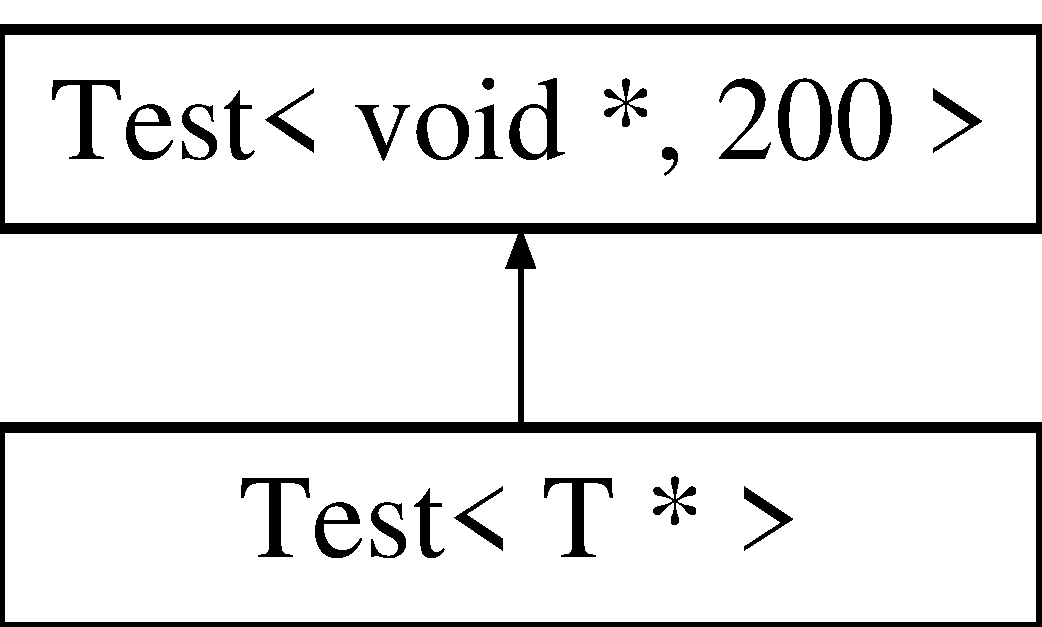
\includegraphics[height=2.000000cm]{class_test_3_01_t_01_5_01_4}
\end{center}
\end{figure}
\subsection*{Public Member Functions}
\begin{DoxyCompactItemize}
\item 
\hyperlink{class_test_3_01_t_01_5_01_4_a474e8a1211308b3f810f9eafced6cbe7}{Test} ()
\end{DoxyCompactItemize}


\subsection{Detailed Description}
\subsubsection*{template$<$class T$>$class Test$<$ T $\ast$ $>$}

\hyperlink{class_a}{A} partial template specialization 

\subsection{Constructor \& Destructor Documentation}
\hypertarget{class_test_3_01_t_01_5_01_4_a474e8a1211308b3f810f9eafced6cbe7}{\index{Test$<$ T $\ast$ $>$@{Test$<$ T $\ast$ $>$}!Test@{Test}}
\index{Test@{Test}!Test< T * >@{Test$<$ T $\ast$ $>$}}
\subsubsection[{Test}]{\setlength{\rightskip}{0pt plus 5cm}template$<$class T $>$ {\bf Test}$<$ T $\ast$ $>$\-::{\bf Test} (
\begin{DoxyParamCaption}
{}
\end{DoxyParamCaption}
)}}\label{class_test_3_01_t_01_5_01_4_a474e8a1211308b3f810f9eafced6cbe7}
The constructor of the partial specilization 

The documentation for this class was generated from the following file\-:\begin{DoxyCompactItemize}
\item 
templ.\-cpp\end{DoxyCompactItemize}

\hypertarget{class_test_3_01void_01_5_00_01200_01_4}{\section{Test$<$ void $\ast$, 200 $>$ Class Template Reference}
\label{class_test_3_01void_01_5_00_01200_01_4}\index{Test$<$ void $\ast$, 200 $>$@{Test$<$ void $\ast$, 200 $>$}}
}
Inheritance diagram for Test$<$ void $\ast$, 200 $>$\-:\begin{figure}[H]
\begin{center}
\leavevmode
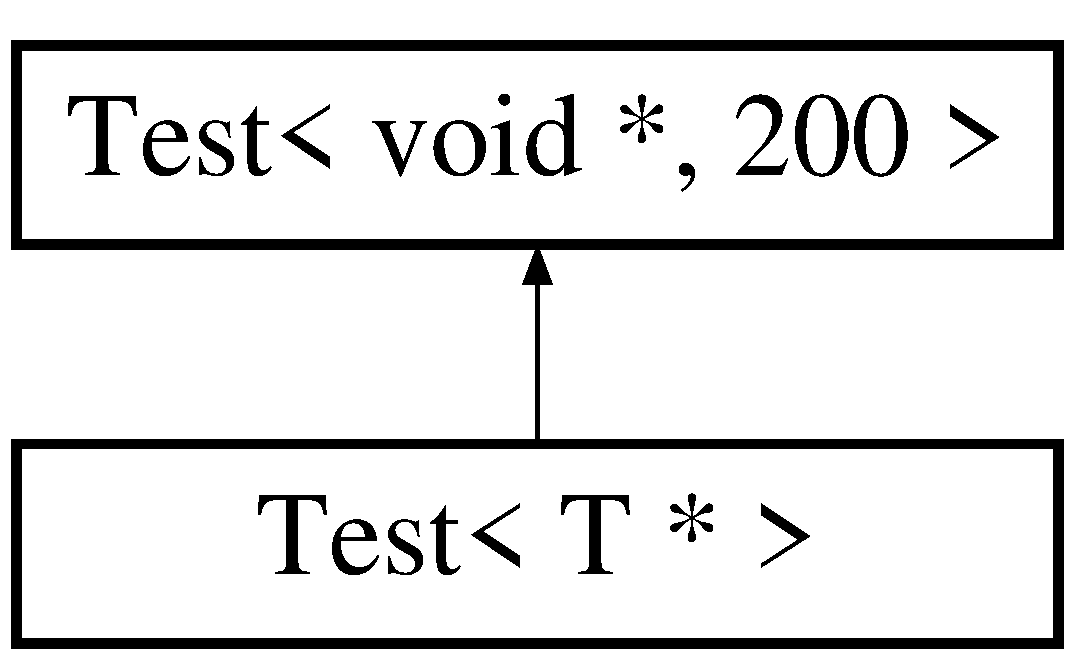
\includegraphics[height=2.000000cm]{class_test_3_01void_01_5_00_01200_01_4}
\end{center}
\end{figure}
\subsection*{Public Member Functions}
\begin{DoxyCompactItemize}
\item 
\hyperlink{class_test_3_01void_01_5_00_01200_01_4_aef160085cc11406b872b45fa871c7692}{Test} ()
\end{DoxyCompactItemize}


\subsection{Detailed Description}
\subsubsection*{template$<$$>$class Test$<$ void $\ast$, 200 $>$}

complete specialization 

\subsection{Constructor \& Destructor Documentation}
\hypertarget{class_test_3_01void_01_5_00_01200_01_4_aef160085cc11406b872b45fa871c7692}{\index{Test$<$ void $\ast$, 200 $>$@{Test$<$ void $\ast$, 200 $>$}!Test@{Test}}
\index{Test@{Test}!Test< void *, 200 >@{Test$<$ void $\ast$, 200 $>$}}
\subsubsection[{Test}]{\setlength{\rightskip}{0pt plus 5cm}{\bf Test}$<$ void $\ast$, 200 $>$\-::{\bf Test} (
\begin{DoxyParamCaption}
{}
\end{DoxyParamCaption}
)}}\label{class_test_3_01void_01_5_00_01200_01_4_aef160085cc11406b872b45fa871c7692}
The constructor of the specilization 

The documentation for this class was generated from the following file\-:\begin{DoxyCompactItemize}
\item 
templ.\-cpp\end{DoxyCompactItemize}

\hypertarget{struct_truck}{\section{Truck Struct Reference}
\label{struct_truck}\index{Truck@{Truck}}
}
Inheritance diagram for Truck\-:\begin{figure}[H]
\begin{center}
\leavevmode
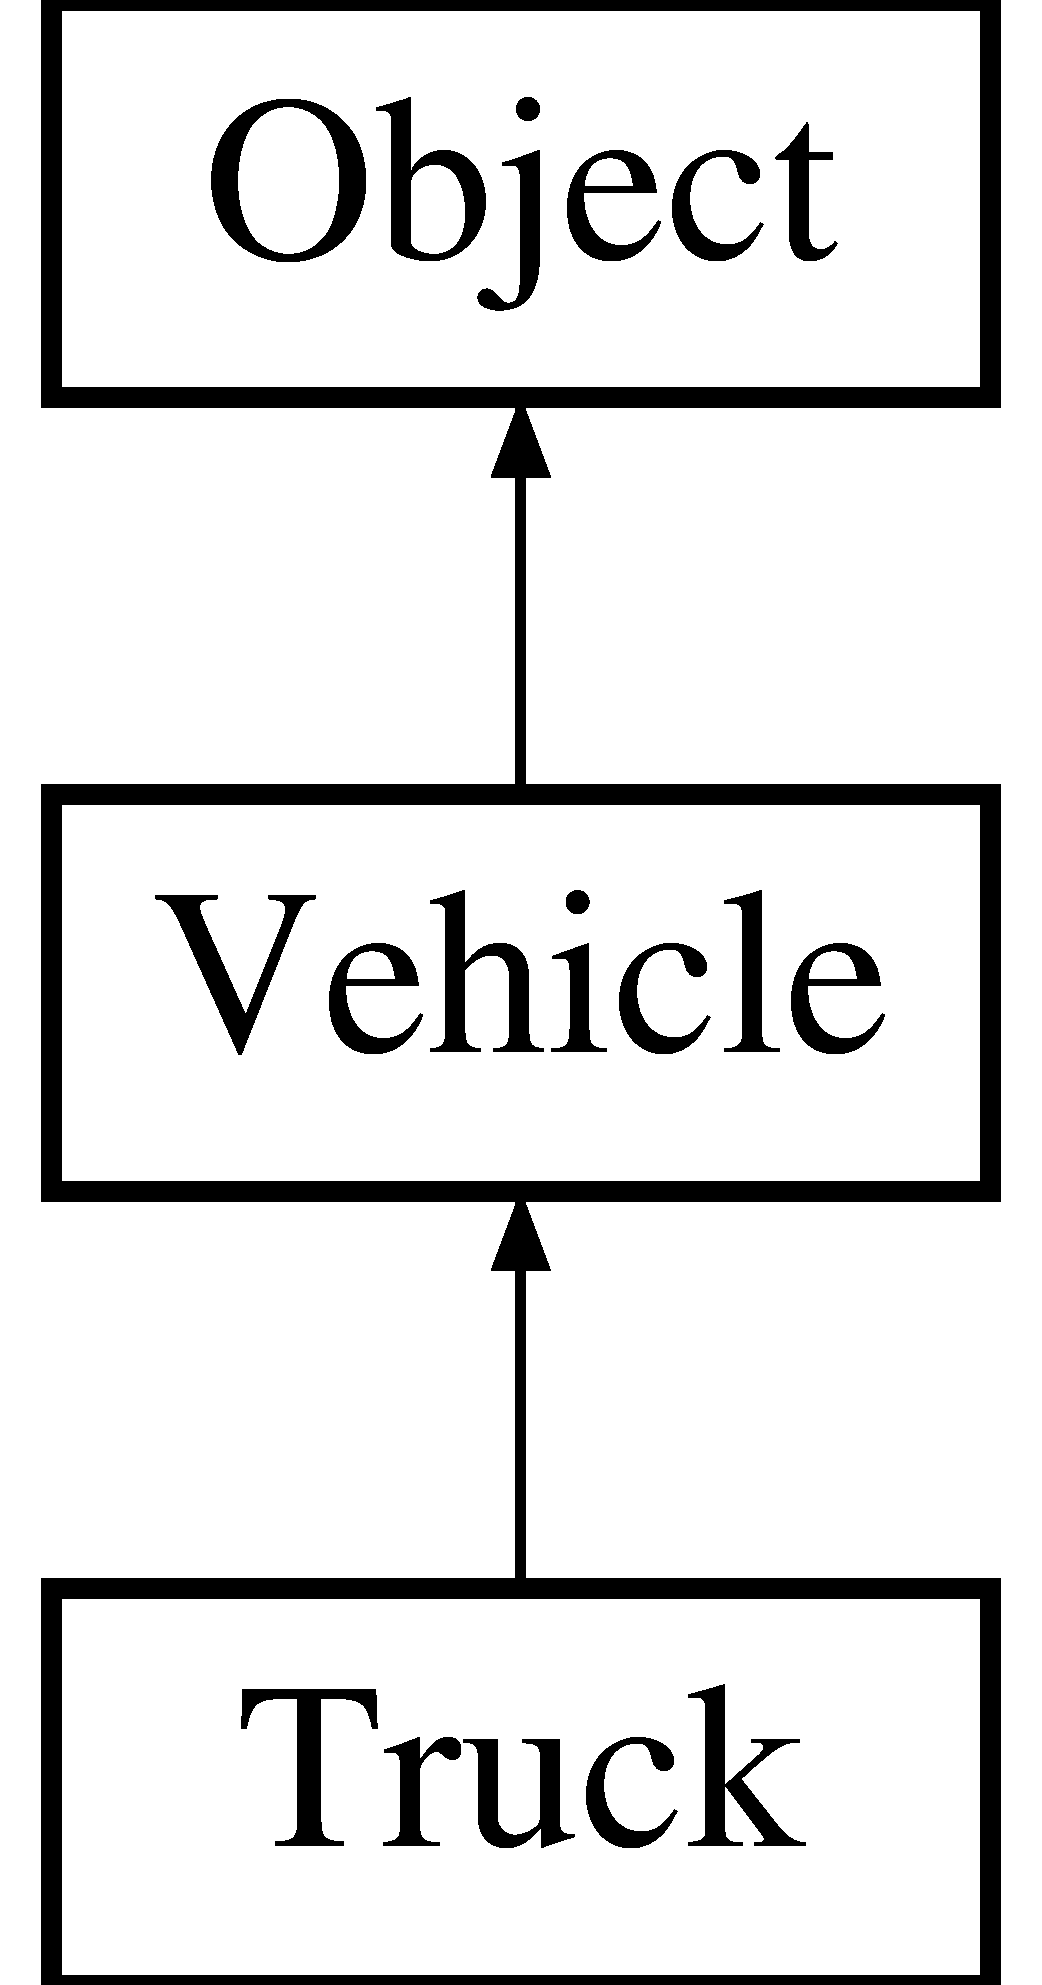
\includegraphics[height=3.000000cm]{struct_truck}
\end{center}
\end{figure}
\subsection*{Protected Attributes}
\begin{DoxyCompactItemize}
\item 
\hypertarget{struct_truck_ad0ac321609dda1a6c552488b05ec7ac8}{\hyperlink{struct_vehicle}{Vehicle} \hyperlink{struct_truck_ad0ac321609dda1a6c552488b05ec7ac8}{base}}\label{struct_truck_ad0ac321609dda1a6c552488b05ec7ac8}

\begin{DoxyCompactList}\small\item\em Base class. \end{DoxyCompactList}\end{DoxyCompactItemize}
\subsection*{Additional Inherited Members}


\subsection{Detailed Description}
\hyperlink{struct_truck}{Truck} class. 

The documentation for this struct was generated from the following file\-:\begin{DoxyCompactItemize}
\item 
\hyperlink{manual_8c}{manual.\-c}\end{DoxyCompactItemize}

\hypertarget{struct_vehicle}{\section{Vehicle Struct Reference}
\label{struct_vehicle}\index{Vehicle@{Vehicle}}
}
Inheritance diagram for Vehicle\-:\begin{figure}[H]
\begin{center}
\leavevmode
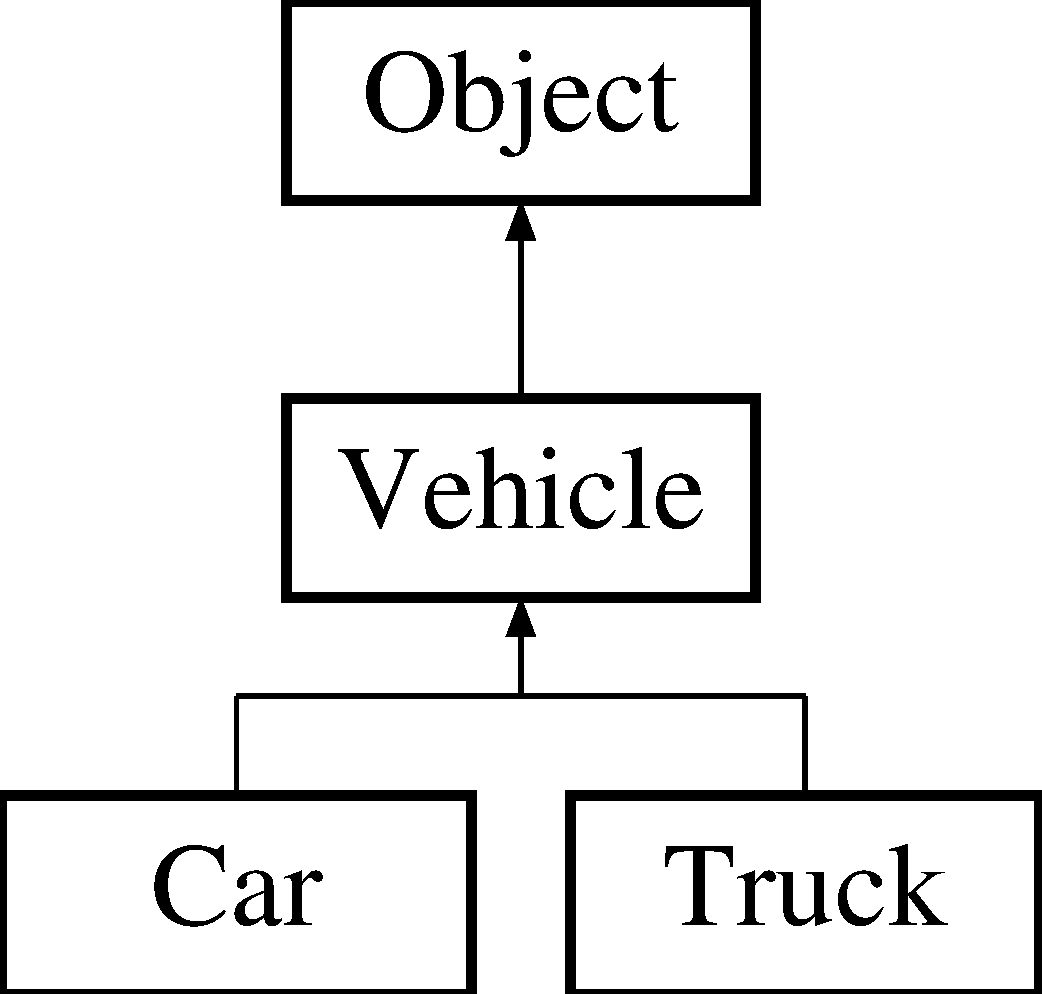
\includegraphics[height=3.000000cm]{struct_vehicle}
\end{center}
\end{figure}
\subsection*{Public Member Functions}
\begin{DoxyCompactItemize}
\item 
void \hyperlink{struct_vehicle_a6891d3d28853bc3fdd075596dc6de9f8}{vehicle\-Start} (\hyperlink{struct_vehicle}{Vehicle} $\ast$obj)
\item 
void \hyperlink{struct_vehicle_a4dcbcba43792dcd673a552b14479ab77}{vehicle\-Stop} (\hyperlink{struct_vehicle}{Vehicle} $\ast$obj)
\end{DoxyCompactItemize}
\subsection*{Protected Attributes}
\begin{DoxyCompactItemize}
\item 
\hypertarget{struct_vehicle_ad7970f528d429f6fc1725173e93a77c2}{\hyperlink{struct_object}{Object} \hyperlink{struct_vehicle_ad7970f528d429f6fc1725173e93a77c2}{base}}\label{struct_vehicle_ad7970f528d429f6fc1725173e93a77c2}

\begin{DoxyCompactList}\small\item\em Base class. \end{DoxyCompactList}\end{DoxyCompactItemize}


\subsection{Detailed Description}
\hyperlink{struct_vehicle}{Vehicle} class. 

\subsection{Member Function Documentation}
\hypertarget{struct_vehicle_a6891d3d28853bc3fdd075596dc6de9f8}{\index{Vehicle@{Vehicle}!vehicle\-Start@{vehicle\-Start}}
\index{vehicle\-Start@{vehicle\-Start}!Vehicle@{Vehicle}}
\subsubsection[{vehicle\-Start}]{\setlength{\rightskip}{0pt plus 5cm}void vehicle\-Start (
\begin{DoxyParamCaption}
\item[{{\bf Vehicle} $\ast$}]{obj}
\end{DoxyParamCaption}
)}}\label{struct_vehicle_a6891d3d28853bc3fdd075596dc6de9f8}
Starts the vehicle. \hypertarget{struct_vehicle_a4dcbcba43792dcd673a552b14479ab77}{\index{Vehicle@{Vehicle}!vehicle\-Stop@{vehicle\-Stop}}
\index{vehicle\-Stop@{vehicle\-Stop}!Vehicle@{Vehicle}}
\subsubsection[{vehicle\-Stop}]{\setlength{\rightskip}{0pt plus 5cm}void vehicle\-Stop (
\begin{DoxyParamCaption}
\item[{{\bf Vehicle} $\ast$}]{obj}
\end{DoxyParamCaption}
)}}\label{struct_vehicle_a4dcbcba43792dcd673a552b14479ab77}
Stops the vehicle. 

The documentation for this struct was generated from the following file\-:\begin{DoxyCompactItemize}
\item 
\hyperlink{manual_8c}{manual.\-c}\end{DoxyCompactItemize}

\chapter{File Documentation}
\hypertarget{autolink_8cpp}{\section{autolink.\-cpp File Reference}
\label{autolink_8cpp}\index{autolink.\-cpp@{autolink.\-cpp}}
}
\subsection*{Classes}
\begin{DoxyCompactItemize}
\item 
class \hyperlink{class_test}{Test$<$ T, i $>$}
\begin{DoxyCompactList}\small\item\em This is a test class. \end{DoxyCompactList}\end{DoxyCompactItemize}
\subsection*{Macros}
\begin{DoxyCompactItemize}
\item 
\#define \hyperlink{autolink_8cpp_a996f7be338ccb40d1a2a5abc1ad61759}{A\-B\-S}(x)~(((x)$>$0)?(x)\-:-\/(x))
\end{DoxyCompactItemize}
\subsection*{Typedefs}
\begin{DoxyCompactItemize}
\item 
\hypertarget{autolink_8cpp_ae0e289308b6d2cbb5c86e753741981dc}{typedef \hyperlink{class_test}{Test} {\bfseries B}}\label{autolink_8cpp_ae0e289308b6d2cbb5c86e753741981dc}

\end{DoxyCompactItemize}
\subsection*{Enumerations}
\begin{DoxyCompactItemize}
\item 
enum \hyperlink{autolink_8cpp_a656d63cf384d2a6f23c2c18523a7bc5e}{Glob\-Enum} \{ \hyperlink{autolink_8cpp_a656d63cf384d2a6f23c2c18523a7bc5ea0f016f49e4f3bcd072319b9d68bc927d}{G\-Val1}, 
\hyperlink{autolink_8cpp_a656d63cf384d2a6f23c2c18523a7bc5ea811876e2eea5c16ae0594a95d98fbd55}{G\-Val2}
 \}
\end{DoxyCompactItemize}
\subsection*{Variables}
\begin{DoxyCompactItemize}
\item 
int \hyperlink{autolink_8cpp_a88d0bae800d600a11d7bd60f0bc4b858}{glob\-Var}
\end{DoxyCompactItemize}


\subsection{Detailed Description}
Testing automatic link generation.

\hyperlink{class_a}{A} link to a member of the \hyperlink{class_test}{Test} class\-: \hyperlink{class_test_a703997077e40c222687a0ea2973a9ea1}{Test\-::member},

More specific links to the each of the overloaded members\-: \hyperlink{class_test_ac2f90eeb597ab8382dcdfcdf1df720f1}{Test\-::member(int)} and \hyperlink{class_test_aea163a1016f022bdb9e4acc3a32fa3eb}{Test\-::member(int,int)}

\hyperlink{class_a}{A} link to a protected member variable of \hyperlink{class_test}{Test}\-: \hyperlink{class_test_ae75d55c8cf6390227d51c0965a4de296}{Test\-::var},

\hyperlink{class_a}{A} link to the global enumeration type \hyperlink{autolink_8cpp_a656d63cf384d2a6f23c2c18523a7bc5e}{Glob\-Enum}.

\hyperlink{class_a}{A} link to the define \hyperlink{autolink_8cpp_a996f7be338ccb40d1a2a5abc1ad61759}{A\-B\-S(x)}.

\hyperlink{class_a}{A} link to the destructor of the \hyperlink{class_test}{Test} class\-: \hyperlink{class_test_a31b169208ad4fc5344a7b6b8e1fd00c1}{Test\-::$\sim$\-Test},

\hyperlink{class_a}{A} link to the typedef \hyperlink{class_b}{B}.

\hyperlink{class_a}{A} link to the enumeration type \hyperlink{class_test_a0653c5125502203305b6fe839e99ed01}{Test\-::\-E\-Type}

\hyperlink{class_a}{A} link to some enumeration values \hyperlink{class_test_ad8d13fe56b896633273087859b89a1a3af621232782128e49458adf9069e126d4}{Test\-::\-Val1} and \hyperlink{autolink_8cpp_a656d63cf384d2a6f23c2c18523a7bc5ea811876e2eea5c16ae0594a95d98fbd55}{G\-Val2} 

\subsection{Macro Definition Documentation}
\hypertarget{autolink_8cpp_a996f7be338ccb40d1a2a5abc1ad61759}{\index{autolink.\-cpp@{autolink.\-cpp}!A\-B\-S@{A\-B\-S}}
\index{A\-B\-S@{A\-B\-S}!autolink.cpp@{autolink.\-cpp}}
\subsubsection[{A\-B\-S}]{\setlength{\rightskip}{0pt plus 5cm}\#define A\-B\-S(
\begin{DoxyParamCaption}
\item[{}]{x}
\end{DoxyParamCaption}
)~(((x)$>$0)?(x)\-:-\/(x))}}\label{autolink_8cpp_a996f7be338ccb40d1a2a5abc1ad61759}
\hyperlink{class_a}{A} macro definition. 

\subsection{Enumeration Type Documentation}
\hypertarget{autolink_8cpp_a656d63cf384d2a6f23c2c18523a7bc5e}{\index{autolink.\-cpp@{autolink.\-cpp}!Glob\-Enum@{Glob\-Enum}}
\index{Glob\-Enum@{Glob\-Enum}!autolink.cpp@{autolink.\-cpp}}
\subsubsection[{Glob\-Enum}]{\setlength{\rightskip}{0pt plus 5cm}enum {\bf Glob\-Enum}}}\label{autolink_8cpp_a656d63cf384d2a6f23c2c18523a7bc5e}
\hyperlink{class_a}{A} global enum. \begin{Desc}
\item[Enumerator\-: ]\par
\begin{description}
\index{G\-Val1@{G\-Val1}!autolink.\-cpp@{autolink.\-cpp}}\index{autolink.\-cpp@{autolink.\-cpp}!G\-Val1@{G\-Val1}}\item[{\em 
\hypertarget{autolink_8cpp_a656d63cf384d2a6f23c2c18523a7bc5ea0f016f49e4f3bcd072319b9d68bc927d}{G\-Val1}\label{autolink_8cpp_a656d63cf384d2a6f23c2c18523a7bc5ea0f016f49e4f3bcd072319b9d68bc927d}
}]global enum value 1 \index{G\-Val2@{G\-Val2}!autolink.\-cpp@{autolink.\-cpp}}\index{autolink.\-cpp@{autolink.\-cpp}!G\-Val2@{G\-Val2}}\item[{\em 
\hypertarget{autolink_8cpp_a656d63cf384d2a6f23c2c18523a7bc5ea811876e2eea5c16ae0594a95d98fbd55}{G\-Val2}\label{autolink_8cpp_a656d63cf384d2a6f23c2c18523a7bc5ea811876e2eea5c16ae0594a95d98fbd55}
}]global enum value 2 \end{description}
\end{Desc}



\subsection{Variable Documentation}
\hypertarget{autolink_8cpp_a88d0bae800d600a11d7bd60f0bc4b858}{\index{autolink.\-cpp@{autolink.\-cpp}!glob\-Var@{glob\-Var}}
\index{glob\-Var@{glob\-Var}!autolink.cpp@{autolink.\-cpp}}
\subsubsection[{glob\-Var}]{\setlength{\rightskip}{0pt plus 5cm}int glob\-Var}}\label{autolink_8cpp_a88d0bae800d600a11d7bd60f0bc4b858}
\hyperlink{class_a}{A} global variable. 
\hypertarget{define_8h}{\section{define.\-h File Reference}
\label{define_8h}\index{define.\-h@{define.\-h}}
}


testing defines  


\subsection*{Macros}
\begin{DoxyCompactItemize}
\item 
\#define \hyperlink{define_8h_a996f7be338ccb40d1a2a5abc1ad61759}{A\-B\-S}(x)~(((x)$>$0)?(x)\-:-\/(x))
\item 
\#define \hyperlink{define_8h_aacc3ee1a7f283f8ef65cea31f4436a95}{M\-A\-X}(x, y)~((x)$>$(y)?(x)\-:(y))
\item 
\#define \hyperlink{define_8h_a74e75242132eaabbc1c512488a135926}{M\-I\-N}(x, y)~((x)$>$(y)?(y)\-:(x))
\end{DoxyCompactItemize}


\subsection{Detailed Description}
testing defines This is to test the documentation of defines. 

\subsection{Macro Definition Documentation}
\hypertarget{define_8h_a996f7be338ccb40d1a2a5abc1ad61759}{\index{define.\-h@{define.\-h}!A\-B\-S@{A\-B\-S}}
\index{A\-B\-S@{A\-B\-S}!define.h@{define.\-h}}
\subsubsection[{A\-B\-S}]{\setlength{\rightskip}{0pt plus 5cm}\#define A\-B\-S(
\begin{DoxyParamCaption}
\item[{}]{x}
\end{DoxyParamCaption}
)~(((x)$>$0)?(x)\-:-\/(x))}}\label{define_8h_a996f7be338ccb40d1a2a5abc1ad61759}
Computes the absolute value of its argument {\itshape x}. \hypertarget{define_8h_aacc3ee1a7f283f8ef65cea31f4436a95}{\index{define.\-h@{define.\-h}!M\-A\-X@{M\-A\-X}}
\index{M\-A\-X@{M\-A\-X}!define.h@{define.\-h}}
\subsubsection[{M\-A\-X}]{\setlength{\rightskip}{0pt plus 5cm}\#define M\-A\-X(
\begin{DoxyParamCaption}
\item[{}]{x, }
\item[{}]{y}
\end{DoxyParamCaption}
)~((x)$>$(y)?(x)\-:(y))}}\label{define_8h_aacc3ee1a7f283f8ef65cea31f4436a95}
Computes the maximum of {\itshape x} and {\itshape y}. \hypertarget{define_8h_a74e75242132eaabbc1c512488a135926}{\index{define.\-h@{define.\-h}!M\-I\-N@{M\-I\-N}}
\index{M\-I\-N@{M\-I\-N}!define.h@{define.\-h}}
\subsubsection[{M\-I\-N}]{\setlength{\rightskip}{0pt plus 5cm}\#define M\-I\-N(
\begin{DoxyParamCaption}
\item[{}]{x, }
\item[{}]{y}
\end{DoxyParamCaption}
)~((x)$>$(y)?(y)\-:(x))}}\label{define_8h_a74e75242132eaabbc1c512488a135926}
Computes the minimum of {\itshape x} and {\itshape y}. 
\hypertarget{file_8h}{\section{file.\-h File Reference}
\label{file_8h}\index{file.\-h@{file.\-h}}
}
\subsection*{Variables}
\begin{DoxyCompactItemize}
\item 
int \hyperlink{file_8h_a4a86bef4b6181cb3f53bd0461a9a511b}{global\-Value}
\end{DoxyCompactItemize}


\subsection{Detailed Description}
\hyperlink{class_a}{A} brief file description. \hyperlink{class_a}{A} more elaborated file description. 

\subsection{Variable Documentation}
\hypertarget{file_8h_a4a86bef4b6181cb3f53bd0461a9a511b}{\index{file.\-h@{file.\-h}!global\-Value@{global\-Value}}
\index{global\-Value@{global\-Value}!file.h@{file.\-h}}
\subsubsection[{global\-Value}]{\setlength{\rightskip}{0pt plus 5cm}int global\-Value}}\label{file_8h_a4a86bef4b6181cb3f53bd0461a9a511b}
\hyperlink{class_a}{A} global integer value. More details about this value. 
\hypertarget{group_8cpp}{\section{group.\-cpp File Reference}
\label{group_8cpp}\index{group.\-cpp@{group.\-cpp}}
}


this file in group 3  


\subsection*{Classes}
\begin{DoxyCompactItemize}
\item 
class \hyperlink{class_c1}{C1}
\begin{DoxyCompactList}\small\item\em class \hyperlink{class_c1}{C1} in group 1 \end{DoxyCompactList}\item 
class \hyperlink{class_c2}{C2}
\begin{DoxyCompactList}\small\item\em class \hyperlink{class_c2}{C2} in group 1 \end{DoxyCompactList}\item 
class \hyperlink{class_c3}{C3}
\begin{DoxyCompactList}\small\item\em class \hyperlink{class_c3}{C3} in group 2 \end{DoxyCompactList}\item 
class \hyperlink{class_c4}{C4}
\begin{DoxyCompactList}\small\item\em class \hyperlink{class_c4}{C4} in group 2 \end{DoxyCompactList}\item 
class \hyperlink{class_c5}{C5}
\begin{DoxyCompactList}\small\item\em class \hyperlink{class_c5}{C5} in \hyperlink{group__group3}{the third group}. \end{DoxyCompactList}\end{DoxyCompactItemize}
\subsection*{Namespaces}
\begin{DoxyCompactItemize}
\item 
namespace \hyperlink{namespace_n1}{N1}
\end{DoxyCompactItemize}
\subsection*{Functions}
\begin{DoxyCompactItemize}
\item 
void \hyperlink{group__group1_ga24f647174760cac13d2624b5ad74b00c}{func} ()
\item 
void \hyperlink{group__group1_ga053929c0809a5f56f7548fd7d9968f31}{func2} ()
\item 
void \hyperlink{group__group1_gadbf675591ff057ec48ce35b0d5cdf755}{func3} ()
\end{DoxyCompactItemize}


\subsection{Detailed Description}
this file in group 3 
\hypertarget{manual_8c}{\section{manual.\-c File Reference}
\label{manual_8c}\index{manual.\-c@{manual.\-c}}
}
\subsection*{Classes}
\begin{DoxyCompactItemize}
\item 
struct \hyperlink{struct_object}{Object}
\item 
struct \hyperlink{struct_vehicle}{Vehicle}
\item 
struct \hyperlink{struct_car}{Car}
\item 
struct \hyperlink{struct_truck}{Truck}
\end{DoxyCompactItemize}
\subsection*{Typedefs}
\begin{DoxyCompactItemize}
\item 
\hypertarget{manual_8c_ab1287b6141419421dc5c14b9f7756b0a}{typedef struct \hyperlink{struct_object}{Object} \hyperlink{manual_8c_ab1287b6141419421dc5c14b9f7756b0a}{Object}}\label{manual_8c_ab1287b6141419421dc5c14b9f7756b0a}

\begin{DoxyCompactList}\small\item\em \hyperlink{struct_object}{Object} type. \end{DoxyCompactList}\item 
\hypertarget{manual_8c_abe36c46f351fd80b9dd6401e7cce0b5d}{typedef struct \hyperlink{struct_vehicle}{Vehicle} \hyperlink{manual_8c_abe36c46f351fd80b9dd6401e7cce0b5d}{Vehicle}}\label{manual_8c_abe36c46f351fd80b9dd6401e7cce0b5d}

\begin{DoxyCompactList}\small\item\em \hyperlink{struct_vehicle}{Vehicle} type. \end{DoxyCompactList}\item 
\hypertarget{manual_8c_a00b00bef7a37e8519a62cb3671105c4b}{typedef struct \hyperlink{struct_car}{Car} \hyperlink{manual_8c_a00b00bef7a37e8519a62cb3671105c4b}{Car}}\label{manual_8c_a00b00bef7a37e8519a62cb3671105c4b}

\begin{DoxyCompactList}\small\item\em \hyperlink{struct_car}{Car} type. \end{DoxyCompactList}\item 
\hypertarget{manual_8c_a5220977c04e056b0efcc59a2f05d89a2}{typedef struct \hyperlink{struct_truck}{Truck} \hyperlink{manual_8c_a5220977c04e056b0efcc59a2f05d89a2}{Truck}}\label{manual_8c_a5220977c04e056b0efcc59a2f05d89a2}

\begin{DoxyCompactList}\small\item\em \hyperlink{struct_truck}{Truck} type. \end{DoxyCompactList}\end{DoxyCompactItemize}
\subsection*{Functions}
\begin{DoxyCompactItemize}
\item 
int \hyperlink{manual_8c_a840291bc02cba5474a4cb46a9b9566fe}{main} (void)
\end{DoxyCompactItemize}


\subsection{Function Documentation}
\hypertarget{manual_8c_a840291bc02cba5474a4cb46a9b9566fe}{\index{manual.\-c@{manual.\-c}!main@{main}}
\index{main@{main}!manual.c@{manual.\-c}}
\subsubsection[{main}]{\setlength{\rightskip}{0pt plus 5cm}int main (
\begin{DoxyParamCaption}
\item[{void}]{}
\end{DoxyParamCaption}
)}}\label{manual_8c_a840291bc02cba5474a4cb46a9b9566fe}
Main function.

Ref \hyperlink{struct_vehicle_a6891d3d28853bc3fdd075596dc6de9f8}{vehicle\-Start()}, \hyperlink{struct_object_a71225073d06a793b9a6ea9263ed37b12}{obj\-Ref()}, \hyperlink{struct_object_a924ee0cecc906d148022b3f0d6325cfb}{obj\-Unref()}. 
\hypertarget{memgrp_8cpp}{\section{memgrp.\-cpp File Reference}
\label{memgrp_8cpp}\index{memgrp.\-cpp@{memgrp.\-cpp}}
}
\subsection*{Classes}
\begin{DoxyCompactItemize}
\item 
class \hyperlink{class_test}{Test$<$ T, i $>$}
\begin{DoxyCompactList}\small\item\em This is a test class. \end{DoxyCompactList}\end{DoxyCompactItemize}
\begin{DoxyCompactItemize}
\item 
\#define \hyperlink{memgrp_8cpp_a955f504eccf76b4eb2489c0adab03121}{A}~1
\item 
\#define \hyperlink{memgrp_8cpp_ae0e289308b6d2cbb5c86e753741981dc}{B}~2
\item 
\hypertarget{memgrp_8cpp_a36cb413747454fcdba9dd7b8f972fcf3}{void {\bfseries glob\-\_\-func} ()}\label{memgrp_8cpp_a36cb413747454fcdba9dd7b8f972fcf3}

\end{DoxyCompactItemize}


\subsection{Detailed Description}
docs for this file 

\subsection{Macro Definition Documentation}
\hypertarget{memgrp_8cpp_a955f504eccf76b4eb2489c0adab03121}{\index{memgrp.\-cpp@{memgrp.\-cpp}!A@{A}}
\index{A@{A}!memgrp.cpp@{memgrp.\-cpp}}
\subsubsection[{A}]{\setlength{\rightskip}{0pt plus 5cm}\#define {\bf A}~1}}\label{memgrp_8cpp_a955f504eccf76b4eb2489c0adab03121}
one description for all members of this group (because D\-I\-S\-T\-R\-I\-B\-U\-T\-E\-\_\-\-G\-R\-O\-U\-P\-\_\-\-D\-O\-C is Y\-E\-S in the config file) \hypertarget{memgrp_8cpp_ae0e289308b6d2cbb5c86e753741981dc}{\index{memgrp.\-cpp@{memgrp.\-cpp}!B@{B}}
\index{B@{B}!memgrp.cpp@{memgrp.\-cpp}}
\subsubsection[{B}]{\setlength{\rightskip}{0pt plus 5cm}typedef {\bf Test} {\bf B}~2}}\label{memgrp_8cpp_ae0e289308b6d2cbb5c86e753741981dc}
\hyperlink{class_a}{A} type definition. 
\hypertarget{mux_8vhdl}{\section{mux.\-vhdl File Reference}
\label{mux_8vhdl}\index{mux.\-vhdl@{mux.\-vhdl}}
}


2\-:1 Mux using with-\/select  


\subsection*{Entities}
\begin{DoxyCompactItemize}
\item 
\hyperlink{classmux__using__with}{mux\-\_\-using\-\_\-with} entity
\begin{DoxyCompactList}\small\item\em Mux entity brief description. \end{DoxyCompactList}\end{DoxyCompactItemize}


\subsection{Detailed Description}
2\-:1 Mux using with-\/select 
\hypertarget{restypedef_8cpp}{\section{restypedef.\-cpp File Reference}
\label{restypedef_8cpp}\index{restypedef.\-cpp@{restypedef.\-cpp}}
}
\subsection*{Classes}
\begin{DoxyCompactItemize}
\item 
struct \hyperlink{struct_coord_struct}{Coord\-Struct}
\end{DoxyCompactItemize}
\subsection*{Typedefs}
\begin{DoxyCompactItemize}
\item 
typedef \hyperlink{struct_coord_struct}{Coord\-Struct} \hyperlink{restypedef_8cpp_a013489fb99c6a5b012db8ec66544a507}{Coord}
\end{DoxyCompactItemize}
\subsection*{Functions}
\begin{DoxyCompactItemize}
\item 
\hyperlink{restypedef_8cpp_a013489fb99c6a5b012db8ec66544a507}{Coord} \hyperlink{restypedef_8cpp_a102acaaa258e937adf910898c6133545}{add} (\hyperlink{restypedef_8cpp_a013489fb99c6a5b012db8ec66544a507}{Coord} c1, \hyperlink{restypedef_8cpp_a013489fb99c6a5b012db8ec66544a507}{Coord} c2)
\end{DoxyCompactItemize}


\subsection{Detailed Description}
An example of resolving typedefs. 

\subsection{Typedef Documentation}
\hypertarget{restypedef_8cpp_a013489fb99c6a5b012db8ec66544a507}{\index{restypedef.\-cpp@{restypedef.\-cpp}!Coord@{Coord}}
\index{Coord@{Coord}!restypedef.cpp@{restypedef.\-cpp}}
\subsubsection[{Coord}]{\setlength{\rightskip}{0pt plus 5cm}typedef {\bf Coord\-Struct} {\bf Coord}}}\label{restypedef_8cpp_a013489fb99c6a5b012db8ec66544a507}
Creates a type name for \hyperlink{struct_coord_struct}{Coord\-Struct} 

\subsection{Function Documentation}
\hypertarget{restypedef_8cpp_a102acaaa258e937adf910898c6133545}{\index{restypedef.\-cpp@{restypedef.\-cpp}!add@{add}}
\index{add@{add}!restypedef.cpp@{restypedef.\-cpp}}
\subsubsection[{add}]{\setlength{\rightskip}{0pt plus 5cm}{\bf Coord} add (
\begin{DoxyParamCaption}
\item[{{\bf Coord}}]{c1, }
\item[{{\bf Coord}}]{c2}
\end{DoxyParamCaption}
)}}\label{restypedef_8cpp_a102acaaa258e937adf910898c6133545}
This function returns the addition of {\itshape c1} and {\itshape c2}, i.\-e\-: (c1.\-x+c2.x,c1.\-y+c2.y) 
\hypertarget{structcmd_8h}{\section{structcmd.\-h File Reference}
\label{structcmd_8h}\index{structcmd.\-h@{structcmd.\-h}}
}


\hyperlink{class_a}{A} Documented file.  


\subsection*{Macros}
\begin{DoxyCompactItemize}
\item 
\#define \hyperlink{structcmd_8h_afa99ec4acc4ecb2dc3c2d05da15d0e3f}{M\-A\-X}(a, b)~(((a)$>$(b))?(a)\-:(b))
\begin{DoxyCompactList}\small\item\em \hyperlink{class_a}{A} macro that returns the maximum of {\itshape a} and {\itshape b}. \end{DoxyCompactList}\end{DoxyCompactItemize}
\subsection*{Typedefs}
\begin{DoxyCompactItemize}
\item 
typedef unsigned int \hyperlink{structcmd_8h_ae1e6edbbc26d6fbc71a90190d0266018}{U\-I\-N\-T32}
\begin{DoxyCompactList}\small\item\em \hyperlink{class_a}{A} type definition for a . \end{DoxyCompactList}\end{DoxyCompactItemize}
\subsection*{Functions}
\begin{DoxyCompactItemize}
\item 
int \hyperlink{structcmd_8h_a2c4414339f388561554c2deab11a1a07}{open} (const char $\ast$, int)
\begin{DoxyCompactList}\small\item\em Opens a file descriptor. \end{DoxyCompactList}\item 
int \hyperlink{structcmd_8h_ae152484c890a24e4d9b4980e7b965be0}{close} (int)
\begin{DoxyCompactList}\small\item\em Closes the file descriptor {\itshape fd}. \end{DoxyCompactList}\item 
size\-\_\-t \hyperlink{structcmd_8h_af2a3ea719b83f672637febdd87c36c36}{write} (int, const char $\ast$, size\-\_\-t)
\begin{DoxyCompactList}\small\item\em Writes {\itshape count} bytes from {\itshape buf} to the filedescriptor {\itshape fd}. \end{DoxyCompactList}\item 
int \hyperlink{structcmd_8h_a9c7b76d5266903891c803132d51ccb90}{read} (int, char $\ast$, size\-\_\-t)
\begin{DoxyCompactList}\small\item\em Read bytes from a file descriptor. \end{DoxyCompactList}\end{DoxyCompactItemize}
\subsection*{Variables}
\begin{DoxyCompactItemize}
\item 
int \hyperlink{structcmd_8h_ad65a8842cc674e3ddf69355898c0ecbf}{errno}
\begin{DoxyCompactList}\small\item\em Contains the last error code. \end{DoxyCompactList}\end{DoxyCompactItemize}


\subsection{Detailed Description}
\hyperlink{class_a}{A} Documented file. Details. 

\subsection{Macro Definition Documentation}
\hypertarget{structcmd_8h_afa99ec4acc4ecb2dc3c2d05da15d0e3f}{\index{structcmd.\-h@{structcmd.\-h}!M\-A\-X@{M\-A\-X}}
\index{M\-A\-X@{M\-A\-X}!structcmd.h@{structcmd.\-h}}
\subsubsection[{M\-A\-X}]{\setlength{\rightskip}{0pt plus 5cm}\#define M\-A\-X(
\begin{DoxyParamCaption}
\item[{}]{a, }
\item[{}]{b}
\end{DoxyParamCaption}
)~(((a)$>$(b))?(a)\-:(b))}}\label{structcmd_8h_afa99ec4acc4ecb2dc3c2d05da15d0e3f}


\hyperlink{class_a}{A} macro that returns the maximum of {\itshape a} and {\itshape b}. 

Details. 

\subsection{Typedef Documentation}
\hypertarget{structcmd_8h_ae1e6edbbc26d6fbc71a90190d0266018}{\index{structcmd.\-h@{structcmd.\-h}!U\-I\-N\-T32@{U\-I\-N\-T32}}
\index{U\-I\-N\-T32@{U\-I\-N\-T32}!structcmd.h@{structcmd.\-h}}
\subsubsection[{U\-I\-N\-T32}]{\setlength{\rightskip}{0pt plus 5cm}typedef unsigned int {\bf U\-I\-N\-T32}}}\label{structcmd_8h_ae1e6edbbc26d6fbc71a90190d0266018}


\hyperlink{class_a}{A} type definition for a . 

Details. 

\subsection{Function Documentation}
\hypertarget{structcmd_8h_ae152484c890a24e4d9b4980e7b965be0}{\index{structcmd.\-h@{structcmd.\-h}!close@{close}}
\index{close@{close}!structcmd.h@{structcmd.\-h}}
\subsubsection[{close}]{\setlength{\rightskip}{0pt plus 5cm}int close (
\begin{DoxyParamCaption}
\item[{int}]{fd}
\end{DoxyParamCaption}
)}}\label{structcmd_8h_ae152484c890a24e4d9b4980e7b965be0}


Closes the file descriptor {\itshape fd}. 


\begin{DoxyParams}{Parameters}
{\em fd} & The descriptor to close. \\
\hline
\end{DoxyParams}
\hypertarget{structcmd_8h_a2c4414339f388561554c2deab11a1a07}{\index{structcmd.\-h@{structcmd.\-h}!open@{open}}
\index{open@{open}!structcmd.h@{structcmd.\-h}}
\subsubsection[{open}]{\setlength{\rightskip}{0pt plus 5cm}int open (
\begin{DoxyParamCaption}
\item[{const char $\ast$}]{pathname, }
\item[{int}]{flags}
\end{DoxyParamCaption}
)}}\label{structcmd_8h_a2c4414339f388561554c2deab11a1a07}


Opens a file descriptor. 


\begin{DoxyParams}{Parameters}
{\em pathname} & The name of the descriptor. \\
\hline
{\em flags} & Opening flags. \\
\hline
\end{DoxyParams}
\hypertarget{structcmd_8h_a9c7b76d5266903891c803132d51ccb90}{\index{structcmd.\-h@{structcmd.\-h}!read@{read}}
\index{read@{read}!structcmd.h@{structcmd.\-h}}
\subsubsection[{read}]{\setlength{\rightskip}{0pt plus 5cm}int read (
\begin{DoxyParamCaption}
\item[{int}]{fd, }
\item[{char $\ast$}]{buf, }
\item[{size\-\_\-t}]{count}
\end{DoxyParamCaption}
)}}\label{structcmd_8h_a9c7b76d5266903891c803132d51ccb90}


Read bytes from a file descriptor. 


\begin{DoxyParams}{Parameters}
{\em fd} & The descriptor to read from. \\
\hline
{\em buf} & The buffer to read into. \\
\hline
{\em count} & The number of bytes to read. \\
\hline
\end{DoxyParams}
\hypertarget{structcmd_8h_af2a3ea719b83f672637febdd87c36c36}{\index{structcmd.\-h@{structcmd.\-h}!write@{write}}
\index{write@{write}!structcmd.h@{structcmd.\-h}}
\subsubsection[{write}]{\setlength{\rightskip}{0pt plus 5cm}size\-\_\-t write (
\begin{DoxyParamCaption}
\item[{int}]{fd, }
\item[{const char $\ast$}]{buf, }
\item[{size\-\_\-t}]{count}
\end{DoxyParamCaption}
)}}\label{structcmd_8h_af2a3ea719b83f672637febdd87c36c36}


Writes {\itshape count} bytes from {\itshape buf} to the filedescriptor {\itshape fd}. 


\begin{DoxyParams}{Parameters}
{\em fd} & The descriptor to write to. \\
\hline
{\em buf} & The data buffer to write. \\
\hline
{\em count} & The number of bytes to write. \\
\hline
\end{DoxyParams}


\subsection{Variable Documentation}
\hypertarget{structcmd_8h_ad65a8842cc674e3ddf69355898c0ecbf}{\index{structcmd.\-h@{structcmd.\-h}!errno@{errno}}
\index{errno@{errno}!structcmd.h@{structcmd.\-h}}
\subsubsection[{errno}]{\setlength{\rightskip}{0pt plus 5cm}int errno}}\label{structcmd_8h_ad65a8842cc674e3ddf69355898c0ecbf}


Contains the last error code. 

\begin{DoxyWarning}{Warning}
Not thread safe! 
\end{DoxyWarning}

\hypertarget{tclexample_8tcl}{\section{tclexample.\-tcl File Reference}
\label{tclexample_8tcl}\index{tclexample.\-tcl@{tclexample.\-tcl}}
}
\subsection*{Classes}
\begin{DoxyCompactItemize}
\item 
class \hyperlink{classns_1_1itcl__class}{ns\-::itcl\-\_\-class}
\item 
class \hyperlink{classns_1_1oo__class}{ns\-::oo\-\_\-class}
\end{DoxyCompactItemize}
\subsection*{Namespaces}
\begin{DoxyCompactItemize}
\item 
namespace \hyperlink{namespacens}{ns}
\end{DoxyCompactItemize}
\subsection*{Functions}
\begin{DoxyCompactItemize}
\item 
\hyperlink{tclexample_8tcl_a6fd2deb737d7421831004f9302f451ee}{glob\-\_\-proc} arg
\item 
\hyperlink{namespacens_a1429cbe84d32b17ea4783e5c5c00615b}{ns\-::ns\-\_\-proc} arg
\end{DoxyCompactItemize}


\subsection{Detailed Description}
File documentation.

\begin{DoxyVerb}# Startup code:\
exec tclsh "$0" "$@"\end{DoxyVerb}
 

\subsection{Function Documentation}
\hypertarget{tclexample_8tcl_a6fd2deb737d7421831004f9302f451ee}{\index{tclexample.\-tcl@{tclexample.\-tcl}!glob\-\_\-proc@{glob\-\_\-proc}}
\index{glob\-\_\-proc@{glob\-\_\-proc}!tclexample.tcl@{tclexample.\-tcl}}
\subsubsection[{glob\-\_\-proc}]{\setlength{\rightskip}{0pt plus 5cm}glob\-\_\-proc {arg }
}}\label{tclexample_8tcl_a6fd2deb737d7421831004f9302f451ee}
Documented global proc {\ttfamily glob\-\_\-proc} . param\mbox{[}in\mbox{]} arg Argument 
\chapter{Example Documentation}
\hypertarget{example_test_8cpp-example}{\section{example\-\_\-test.\-cpp}
}
This is an example of how to use the \hyperlink{class_test}{Test} class. More details about this example.


\begin{DoxyCodeInclude}
\end{DoxyCodeInclude}
 
\addcontentsline{toc}{part}{Index}
\printindex
\end{document}
